\RequirePackage[l2tabu, orthodox]{nag}

\documentclass[a4paper, 12pt, DIV=10, ngerman, abstracton, toc=bibliography, toc=listof]{scrreprt}

% compatibility
\usepackage{scrhack} % silences certain KOMA warnings
\usepackage{xltxtra} % fixes XeTeX stuff

% language support
\usepackage[ngerman]{babel}

% bibliography
\usepackage[backend=biber, style=alphabetic]{biblatex}
\bibliography{bibliography.bib}

% fonts
\defaultfontfeatures{Ligatures=TeX}
\setmainfont{Minion Pro}
\setsansfont{Myriad Pro}
\setmonofont{Consolas}
\urlstyle{same}

% line spacing
\usepackage{setspace} 
\setstretch{1.3}

% no paragraph indentation
\parskip 6pt
\parindent 0pt

% no widows
\usepackage[all]{nowidow}

\usepackage{xcolor}
\definecolor{lightgray}{gray}{0.96}

% listings
\usepackage{listings}
\lstset{
    basicstyle=\ttfamily\scriptsize,
    captionpos=b,
    frame=bt,
    numbers=left,
    numberstyle=\rmfamily\tiny\color{gray!50!black},
    keywordstyle=\bfseries,
    % backgroundcolor=\color{lightgray},
    stringstyle=\slshape,
    xleftmargin=8mm,
    framexleftmargin=8mm,
    aboveskip=\baselineskip,
    showspaces=false,
    showtabs=false
}

\lstdefinelanguage{json}{
  morestring=[b]",
}

\lstdefinelanguage{pseudo}{
    keywords={var, foreach, in, function, return, end, do},
}

% referencing stuff
\usepackage[strict=true]{csquotes}
\PassOptionsToPackage{hyphens}{url}\usepackage{hyperref}
\usepackage{cleveref}
\usepackage[font=small,labelfont=bf]{caption}
\captionsetup{%
  figurewithin=chapter,
  tablewithin=chapter
}

% various extensions
\usepackage{siunitx} % numbers and units
\usepackage{booktabs} % good looking tables
\usepackage{dashrule} % dotted lines
\usepackage{amssymb} % math stuff

% no warnings for underfull boxes in bibliography
\usepackage{etoolbox}
\apptocmd{\sloppy}{\hbadness 10000\relax}{}{}

% graphics directory
\graphicspath{{assets/}}

\begin{document}

\pagenumbering{roman}

% title page
\thispagestyle{plain}
\begin{titlepage}
\begin{center}

\includegraphics[width=5cm]{htwk_logo}\\
\vspace{0.3cm}
\normalsize
Hochschule für Technik, Wirtschaft und Kultur Leipzig\\
Fakultät für Informatik, Mathematik und Naturwissenschaften\\
\vspace{3.2cm}
\huge{\textbf{\textsf{Kookkurrenzbasierte Link Discovery am Beispiel von Produkttags}}}\\
\vspace{1cm}
\LARGE{\textsf{Masterarbeit}}\\
\vspace{3.2cm}
\normalsize
Sebastian Marr\\
mail@sebastianmarr.de\\
Leipzig, den \today\\
\vspace{3.2cm}
Erstgutachter: Dr.--Ing. Toralf Kirsten \\
Zweitgutachter: M.Sc. Martin Breest
\end{center}
\end{titlepage}

\begin{abstract}
Durch die Möglichkeit der Benutzerbeteiligung an der Beschreibung, Bewertung und Kategorisierung von Inhalten auf Online-Plattformen werden Begriffswelten aufgebaut, deren Auswertung großes Potenzial für die Verbesserung der Benutzererfahrung bietet. Diese Masterarbeit beschreibt ein Verfahren zum Finden von Zusammenhängen zwischen diesen Begriffen. Grundlage dafür stellen die Daten eines Tagging--Systems und die Ermittlung von Kookkurrenz dar. Die Begriffe und ihre Zusammenhänge werden in eine Graphenrepräsentation transformiert und durch Mining und Integration weiterer Datenquellen angereichert. Zur Priorisierung der Beziehungen für einen Anwendungsfall wird ein Verfahren mittels interaktiver evolutionärer Algorithmen vorstellt und angewendet. Die Ergebnisse der Erzeugung von Beziehungen und der Priorisierung werden präsentiert und schließlich die technische Umsetzung der genannten Verfahren beschrieben.
\end{abstract}
\chapter*{Erklärung}

Ich erkläre hiermit, dass ich diese Masterarbeit selbstständig ohne Hilfe Dritter und ohne Benutzung anderer als der angegebenen Quellen und Hilfsmittel verfasst habe. Alle den benutzten Quellen wörtlich oder sinngemäß entnommenen Stellen sind als solche einzeln kenntlich gemacht.

Diese Arbeit ist bislang keiner anderen Prüfungsbehörde vorgelegt und auch nicht veröffentlicht worden.

Ich bin mir bewusst, dass eine falsche Erklärung rechtliche Folgen haben wird. 

{
\vspace{32pt}
\noindent
\hdashrule{5cm}{1pt}{1pt 3pt}\\
Sebastian Marr\\
Leipzig, den 21. November 2013
}


\tableofcontents

\cleardoublepage

\pagenumbering{arabic}

\chapter{Einleitung}

Mit der steigenden Menge von nutzergenerierten Inhalten steigt auch die Menge von Metadaten, die mit diesen Inhalten verknüpft sind. Zur späteren Durchsuchbarkeit und Kategorisierung geben viele Online-Plattformen, Marktplätze und Online-Shops ihren Benutzern die Möglichkeit, Inhalte mit Metadaten zu versehen.

Eine oft genutzte Möglichkeit zur Beschreibung von Inhalten sind Tags. Dabei handelt es sich um Wörter oder Wortgruppen, die vom Benutzer frei gewählt werden können, um den Inhalt zu beschreiben. Dabei unterliegt die Eingabe von Tags möglichst wenigen Regeln, um dem Benutzer eine für ihn natürliche Beschreibung des Inhaltes zu ermöglichen. Dabei ist explizit, im Gegensatz zu einer Kategorisierung, die Vergabe von mehreren Tags vorgesehen \cite{sc2005}.

Ein charakteristisches Merkmal von Tags ist dabei, dass sie nur einen bestimmten Aspekt des getaggten Objektes beschreiben. Dabei sind Tags nicht hierarchisch und es werden an keiner Stelle vom Nutzer explizite Zusammenhänge zwischen Tags erstellt. Jedoch liegt die Annahme, dass zwischen Tags Beziehungen herstellbar sind und sich mehrere Tags zu übergeordneten Themen zusammenfassen lassen, nahe. Der Benutzer berücksichtigt diese Beziehungen bei der Eingabe des Tags, formuliert sie jedoch nicht explizit. Die nachträgliche Rekonstruktion der Denkprozesse bei der Eingabe von Tags ist Thema dieser Arbeit.

Dabei ist zu beachten, dass Benutzer bei der Eingabe von Tags unterschiedliche Ziele verfolgen. Idealerweise werden Tags so vergeben, dass sie das getaggte Objekt inhaltlich beschreiben. Jedoch werden vom Benutzer bei der eingabe des Tags weitere Assoziationen hergestellt. Beispielsweise kann der Benutzer mit einem Objekt bestimmte Emotionen oder Wertungen verbinden, die sich in den vergebenen Tags wiederspiegeln.

Auf Marktplätzen, bei denen Verkäufern die Möglichkeit des Taggings ihre Produkte gegeben wird, besteht eine weitere Motivation in der Erhöhung der Auffindbarkeit des Produktes. Dabei kann die inhaltliche Qualität des Tags außer Acht gelassen werden, wenn bei Vergabe einer falschen Beschreibung die Sichtbarkeit des Produktes erhöht wird. Auch der Marktplatzbetreiber selbst kann so vorgehen, um zu versuchen, die Gesamtverkäufe zu steigern.

Die verschiedenen Motivationen der Benutzern von Tags erschwerden die nachträgliche Suche nach Assoziationen. Die vorliegende Masterarbeit beschäftigt sich mit Strategien zur Datenaufbereitung und Nutzung externer und interner Datenquellen und deren Integration mit Tag-Daten. Aus diesen Datenquellen wird eine Datenstruktur mit einem Kookurrenzgraphen als Basis aufgebaut und schließlich werden mit Hilfe von Clustering-Algrithmen daraus Themen extrahiert. Außerdem wird eine Evaluation der Ergebnisse und eine Analyse der verwendeten Methoden durchgeführt.

\section{Motivation und Anwendungen}

Die nachträgliche Herstellung von Assoziationen in vorhandenen Tag-Daten bietet einige Nutzungsmöglichkeiten für den Betreiber der Online-Plattform.

Die Beziehungen zwischen Tags können genutzt werden, um Suchergebnisse zu verbessern. Wenn zu einem Suchbegiff weitere relevante Begriffe bekannt sind, können diese im Suchergebnis mit enthalten sein um somit auch Objekte zu finden, die nicht direkt mit dem Suchbegriff getaggt sind. Außerdem können Suchen vom Benutzer mit Hilfe von verwandten Tags verfeinert werden.

Über die Zusammenfassung von Tags zu Themen lässt sich außerdem die Navigation einer Webseite verbessern. Aus den Themen lassen sich Kategorien oder Hierachien von Kategorien erzeugen, die besser den Denkmustern von Benutzern entsprechen. So sind auch Navigationskonzepte denkbar, die nicht hierarchisch, sondern assoziativ aufgebaut sind. Desweiteren können Tag-Assoziationen für Empfehlungssysteme genutzt werden, die einem Kunden zu einem bestimmten Artikel passende andere Artikel vorschlagen.

Im Bereich des Marketings können Beziehungen zwischen Tags genutzt werden, um für bestimmte externe Suchbegriffe spezielle Seiten zu erstellen (Landing Pages), die Inhalte zu diesem Suchbegriff bereitstellen oder Werbung für diese Suchbegriffe zu schalten. Außerdem können mit Hilfe des Kaufinteresses an bestimmten Themen über die Zeit Trends erkannt werden und mit entsprechenden Marketingmaßnahmen darauf reagiert werden.

All diese Anwendungen führen zu einer besseren Erfahrung für den Benutzer der Plattform. Die Präsentation von Daten kann besser auf die Denkmuster und Erwartungshaltungen des Benutzers angepasst werden. Dies führt in Konsequenz zu einem wirtschaftlichen Vorteil für den Plattformbetreiber.

\section{Kontext}

Die vorliegende Masterarbeit wurde im Kontext der sprd.net AG (nachfolgend Spreadshirt) \footnote{\url{http://www.spreadshirt.net}} erstellt. Spreadshirt ist eine E-Commerce-Platform, die es seinen Benutzern erlaubt, personalisierte Textilien und andere Artikel zu gestalten, zu kaufen und zum Verkauf anzubieten. Spreadshirt übernimmt die Produktion und den Versand der Produkte. Ein Produkt bezeichnet hierbei einen Produkttyp, beispielsweise ein T-Shirt, das mit einem oder mehreren Designs bedruckt wurde.

Das Erstellen von Designs und die Konfiguration eines Produktes, also das Positionieren von Designs auf Produkttypen, wird dabei vollständig vom Benutzer durchgeführt. Spreadshirt bietet hierzu sowohl eine Webseite als auch eine API an.

Dabei agieren grundsätzlich zwei Arten von Benutzern mit der Spreadshirt-Plattform: \emph{Kunden} und \emph{Partner}.

Als Kunden werden Benutzer bezeichnet, die Produkte bestellen. Diese Produkte können entweder von ihnen selbst oder von einem Partner erstellt worden sein. 

Partner sind Benutzer, die Designs oder Produkte erstellen und diese zum Verkauf anbieten. Zu diesem Zweck kann der Partner einen eigenen Shop auf der Spreadshirt-Plattform eröffnen. Kunden können in diesem Shop Produkte bestellen und der Partner erhält einen Anteil des Verkaufspreises, während Spreadshirt die Produktion und den Versand an den Kunden übernimmt.

Neben den von Kunden für sich selbst erstellten Produkten und den Partner-Shops existiert ein weiterer Vertriebskanal: der Spreadshirt-Marktplatz. Auf dem Marktplatz können Partner nach ihrer Zustimmung ihre Designs vertreiben. Kunden können nach Motiven suchen, die ihrem Geschmack entsprechen und diese bestellen, mit anderen Motiven kombinieren oder mit Texten versehen.

Das Suchergebnis für Suchen auf dem Marktplatz hängt dabei maßgeblich von den Metadaten ab, die der Partner für seine Designs vergeben hat. Dies birgt auch Risiken: zur besseren Auffindbarkeit ihrer Designs sind Partner dadurch geneigt, populäre Tags zu vergeben, damit sie im Suchergebnis höher gewertet werden. Dies führt zu \emph{Spam} - Tags, die nicht erwünscht sind und den Inhalt des Designs nicht oder falsch beschreiben.

Um also das Ziel zu erreichen, Themen und Assoziationen aus den Tags zu extrahieren, muss dieses spezifische Problem gelöst werden. Spam lässt sich nur schwer unterdrücken, so dass diesem bei der Auswertung der Daten besondere Aufmerksamkeit gewidmet werden muss.

Spreadshirt agiert international, so dass auf sprachliche und kulturelle Unterschiede Rücksicht genommen werden sollte. Viele Themen sind national unterschiedlich besetzt. Dies sollte in den Beziehungen der Tags untereinander wiedergespiegelt werden.

Der Datenbestand der Spreadshirt-Plattform in Europa besteht aus ca. 2 Millionen Tags, 6 Millionen Designs, 14 Millionen Produkten, 6 Millionn registrierten Nutzern und 750000 eröffneten Partner-Shops.

Der Nutzen dieser Arbeit für Spreadshirt besteht vor allem in der Verbesserung der Suche und des Durchstöberns des Marktplatzes. Den Kunden soll erleichtert werden, Designs zu ihren Wunschthemen zu finden, die ihren Vorstellungen entsprechen. Des Weiteren können diverse Marketingmaßnahmen von den Ergebnissen des Clusterings und der Integration der Tags profitieren.

\section{Verwandte Arbeiten}

Die Herstellung von semantischen Beziehungen in Tag-Daten ist Gegenstand vieler Arbeiten. Diese beschäftigen sich meist mit Daten aus sogenannten Folksonomies, also Sammlungen von Tags aus Systemen, bei denen alle Nutzer Inhalte verschlagworten können.

\textcite{bks2006} beschreiben einen auf Kookkurenz basierenden Ansatz, miteinander verwandte Tags zu Clustern zusammenzufassen. Dabei wird die Kookkurenz nicht nur quantitativ, sondern auch durch die Verteilung der Häufigkeiten des gemeinsamen Vorkommens definiert. Dadurch ergeben sich bereits bei Berechnung des Ähnlichkeitsmaßes Cluster, die dann mit einem partitionierenden Algorithmus weiter geteilt werden.

In der Arbeit von \textcite{ps2006} wird ein Ansatz beschrieben, eine Ontologie aus den Daten der Foto-Plattform \emph{Flickr} herzustellen. Dazu wird versucht, ebenfalls auf Basis von Kookkurenzen, nicht nur Cluster von Tags, sondern hierarchische Beziehungen zwischen eben diesen zu ermitteln. Diese Beziehungen werden durch die Analyse der getaggten Inhalte hergestellt, indem ermittelt wird, welche der getaggten Inhalte Teilmengen voneinander sind.

\textcite{kss2010} arbeiten ebenfalls mit dem Ansatz, auf Basis eines Kookkurenzgraphen Cluster von Tags zu bilden. Die Kokkurenz wird mit den bekannten Maßen Dice, Jaccard und Cosinus berechnet. Als Clusteringalgorithmen kommen Single-Link, Complete-Link und Group-Average zum Einsatz. Die Arbeit legt besonderen Wert auf die Rolle der Cluster zur Verbesserung von Suchoberflächen. Daher werden auch Tests mit Benutzern durchgeführt und die Ergebnisse evaluiert.

\section{Aufbau der Arbeit}
\chapter{Tagging--Systeme}
\label{tagging}

Das folgende Kapitel beschäftigt sich mit Tagging--Systemen. Dabei werden die Grundlagen, das Datenmodell und die Arten von Tagging--Systemen erläutert sowie das System von Spreadshirt, das in dieser Arbeit verwendet wurde, genauer erklärt. Dies umfasst die spezifischen Eigenschaften dieses Systems, die Diskussion der Datenqualität sowie das Mengengerüst der vorhandenen Daten.

\section{Grundlagen}
\label{tagging_basics}

\emph{Tags} sind eine Form von Metadaten, also ``Daten über Daten''. Sie erfüllen die Funktion der \emph{Beschreibung} von Dokumenten und werden im Allgemeinen von Benutzern angelegt. Dies steht im Gegensatz zu professionell kuratierten Metadaten wie beispielsweise Bibliothekskatalogen \cite{ma2004}.

Im Allgemeinen sind Tags kurze Schlagworte, die von dem Benutzer, der sie vergibt, frei gewählt werden können. Jedes Dokument kann mit beliebig vielen Tags versehen werden. Dies steht im Gegensatz zu einer festen, vorgegebenen Klassifikation mittels Kategoriebäumen, wie sie beispielsweise in E--Commerce--Systemen üblich sind, um Artikel zu ordnen. In solchen Kategoriebäumen kann ein Dokument üblicherweise nur in einer begrenzten Anzahl von Kategorien, meistens nur in einer, eingeordnet werden.

Die Menge der Tags eines Systems ist nicht hierarchisch geordnet und es bestehen keine explizit formulierten Beziehungen zwischen einzelnen Tags. Somit ergibt sich eine lose Kategorisierung der Dokumente, die, im Gegensatz zu formalen Taxonomien und Ontologien, ständig von den Benutzern erweitert und verändert wird \cite{sc2005}. \textcite{je2004} beschäftigt sich tiefer gehend mit dem Unterschied zwischen starrer Klassifikation und loser Kategorisierung.

Aus dieser Eigenschaft ergeben sich bestimmte Schwächen und Stärken von Tagging--Systemen, die von \textcite{ma2004} definiert wurden. Demnach liegen die Schwächen in der Mehrdeutigkeit von Tags und der mangelnden Kontrolle von Synonymen. Mehrdeutigkeit bezeichnet den Umstand, dass gleiche Tags zur Beschreibung von sehr unterschiedlichen Dokumenten genutzt werden können, da keine Systematik vorgegeben ist. Die mangelnde Kontrolle von Synonymen führt dazu, dass verschiedene Tags verwendet werden, um den gleichen Sachverhalt zu beschreiben.

Zu den von \textcite{ma2004} formulierten Stärken gehören die starke Ausrichtung von Tags an den Gedankengängen der Benutzer und dem einfacheren Durchstöbern von Dokumenten. Da die Tags von den Benutzern eines Systems formuliert werden, spiegeln sie deren Vokabular und deren Gedankengänge wieder. Werden Tags statt zum Finden von konkreten Dokumenten zum Durchstöbern genutzt, bieten sie größere Möglichkeiten, interessante Inhalte zu finden, als in einer starren Kategorisierung.

Tagging--Systeme enthalten demnach implizites Wissen, dass durch Data Mining extrahiert und genutzt werden kann. Im Rahmen dieser Arbeit wurden Tagging--Systeme als Ausgangspunkt für die Link Discovery mittels Kookkurrenz genutzt genutzt (siehe \cref{co-occurence,ld_tags}).

\subsection{Datenmodell von Tagging--Systemen}
\label{tagging_data}

Ein Tagging--System ist allgemein durch ein Tripel \(S=(D, T, U)\) von Mengen, sowie durch die Relation \(R = D \times U \times T\) definiert. 

\(D\) repräsentiert eine Menge von Dokumenten. Ein Dokument \(d\) kann ein beliebiger Datensatz sein, beispielsweise ein Design, Artikel oder Produkt. Die Menge \(U\) stellt alle Benutzer des Systems dar. Ein Benutzer \(u\) ist eine Entität mit beliebigen weiteren Attributen, die jedoch im Kontext des Tagging--Systems nicht weiter betrachtet werden. \(T\) repräsentiert die Menge der Tags. Ein Tag \(t\) ist eine Entität, die als benötigtes Attribut eine Zeichenkette besitzt, die zur Beschreibung von Dokumenten genutzt werden kann. \(T\) bildet das \emph{Vokabular} des Tagging--Systems.

Die Relation \(R\) beschreibt den Vorgang des \emph{Taggings}. Ein Benutzer \(u\) des Systems vergibt einen Tag \(t\) an ein Dokument \(d\), um den Inhalt von \(d\) mit der Zeichenkette von \(t\) zu beschreiben. \(R\) enthält demnach Tripel der Form \((d,t,u)\).

\begin{figure}
\centering
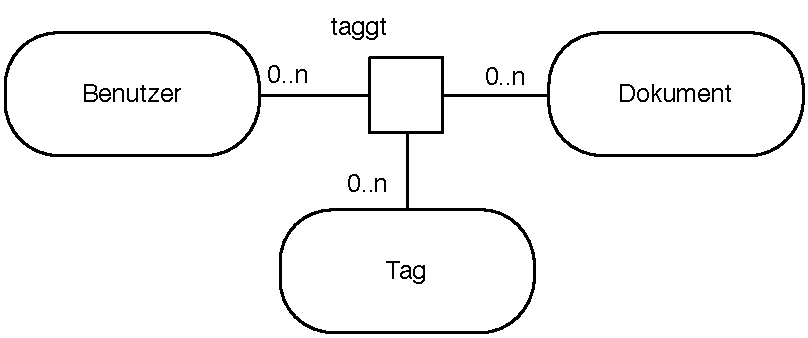
\includegraphics[width=0.75\textwidth]{tag_system}
\caption{FMC--Entity--Relationship--Diagramm eines Tagging--Systems}
\label{fig:tagging_erd}
\end{figure}

Das beschriebene Tagging--System lässt sich somit in ein Datenmodell mit den Entitäten \emph{Benutzer}, \emph{Dokument}, \emph{Tag} und  der ternären Beziehung \emph{Tagging} überführen. Dieses Modell ist in \cref{fig:tagging_erd} als Entity--Relationship--Diagramm dargestellt. Alle genannten Entitäten können weitere Attribute besitzen, die von der Anwendungsdomäne des konkret betrachteten Tagging--Systems abhängen.

\subsection{Arten von Tagging--Systemen}
\label{tagging_types}

Abhängig vom gewünschten Einsatzzweck des Tagging--Systems kann der Betreiber bestimmte Aspekte des Systems beschränken. Außerdem können die Benutzer einen vorherrschenden Umgang mit dem System entwickeln. Aus diesen Faktoren ergeben sich verschiedene Arten und Nutzungsmuster von Tagging-Systemen. Hauptsächlich kann zwischen offenen Tagging--Systemen, den so genannten \emph{Folksonomies} und den teilweise geschlossenen Tagging--Systemen unterschieden werden.

\subsubsection{Folksonomies}

Eine Folksonomy beschreibt ein weitestgehend offenes Tagging--System \cite{ma2004}. Bei dieser Art von System kann grundsätzlich jeder Benutzer jeden Tag an jedes Dokument vergeben. Außerdem stammen die Dokumente selbst meist ebenfalls von den Benutzern. Beispiele für Folksonomies sind der Bookmarking--Dienst \emph{Delicious} \cite{deli} und die Foto-Plattform \emph{Flickr} \cite{flickr}.

Der Begriff \emph{Folksonomy} steht im Gegensatz zur \emph{Taxonomie} und beschreibt den Umstand, dass die Kategorisierung und Ordnung von Inhalten vom \emph{folk}, also den Benutzern selbst vorgenommen werden \cite{vt2007}.

\subsubsection{Teilweise geschlossene Tagging--Systeme}

In teilweise geschlossenen Tagging--Systemen beschränkt der Betreiber des Systems bestimmte Aspekte. Dies können die Benutzer, die Tags vergeben dürfen, die Dokumente oder auch das Vokabular sein.

Eine häufige Form der Einschränkung, der auch das in dieser Arbeit verwendete System unterliegt (siehe \cref{tag_sprd}), ist die Einschränkung der Benutzer die ein Dokument taggen können. Oftmals ist dies nur den Autoren des Dokumentes selbst oder Benutzern mit besonderen Rechten, beispielsweise Moderatoren oder Angestellten des Betreibers, erlaubt.

In den meisten Tagging--Systemen stammen die Dokumente ebenfalls von den Benutzern des Systems, beispielsweise Artikel, Fotos oder Musikstücke. Jedoch kann die Erstellung der Dokumente eingeschränkt werden, wenn dies in der Anwendungsdomäne sinnvoll ist. Beispiele hierfür sind Produkte in Online--Shops. Diese werden nicht von den Benutzern erstellt, jedoch kann die Vergabe von Tags an diese einen Mehrwert liefern.

Die Einschränkung des Vokabulars kann vorgenommen werden, um Rechtschreibfehler und Fehleingaben der Tags zu vermeiden. Sie bringt jedoch den Nachteil mit sich, dass die Tags dann unter Umständen nicht mehr das Vokabular der Benutzer widerspiegeln und somit Inhalte für diese schwerer auffindbar sind.

\section{Tagging--System von Spreadshirt}

Nachdem im vorherigen Abschnitt die Grundlagen von Tagging--Systemen diskutiert wurden, beschäftigt sich dieser Abschnitt mit dem konkreten Tagging--Systems der Website \emph{Spreadshirt}, welches in dieser Arbeit für den initialen Schritt der Link Discovery genutzt wurde (siehe \cref{ld_tags}).

\subsection{Spreadshirt}
\label{spreadshirt}

Die vorliegende Masterarbeit wurde im Kontext der sprd.net AG (Spreadshirt) \cite{sprd2013} erstellt. Spreadshirt ist eine E--Commerce--Plattform, die es seinen Benutzern erlaubt, personalisierte Textilien und andere Artikel zu gestalten, zu kaufen und zum Verkauf anzubieten. Spreadshirt übernimmt die Produktion und den Versand der Produkte. Ein Produkt bezeichnet hierbei einen Produkttyp, beispielsweise ein T--Shirt, der mit einem oder mehreren Designs bedruckt wurde.

Das Erstellen von Designs und die Konfiguration eines Produktes, also das Positionieren von Designs auf Produkttypen, wird vollständig vom Benutzer durchgeführt. Es agieren grundsätzlich zwei Arten von Benutzern mit der Spreadshirt--Plattform: \emph{Kunden} und \emph{Partner}.

Als Kunden werden Benutzer bezeichnet, die Produkte bestellen. Diese Produkte können entweder von ihnen selbst oder von einem Partner erstellt worden sein. 

Partner sind Benutzer, die Designs oder Produkte erstellen und diese zum Verkauf anbieten. Zu diesem Zweck kann der Partner einen eigenen Shop auf der Spreadshirt--Plattform eröffnen. Kunden können in diesem Shop Produkte bestellen und der Partner erhält einen Anteil des Verkaufspreises, während Spreadshirt die Produktion und den Versand an den Kunden übernimmt.

Neben den von Kunden für sich selbst erstellten Produkten und den Partner--Shops existiert mit dem Spreadshirt--Marktplatz ein weiterer Vertriebskanal. Auf dem Marktplatz können Partner nach ihrer Zustimmung ihre Designs vertreiben. Kunden können nach Motiven suchen, die ihrem Geschmack entsprechen und diese bestellen, mit anderen Motiven kombinieren oder mit Texten versehen. Ein Produkt, das entweder in einem Partner--Shop oder auf dem Marktplatz positioniert und mit einem Preis versehen wurde, wird Artikel genannt.

\begin{figure}[t]
\centering
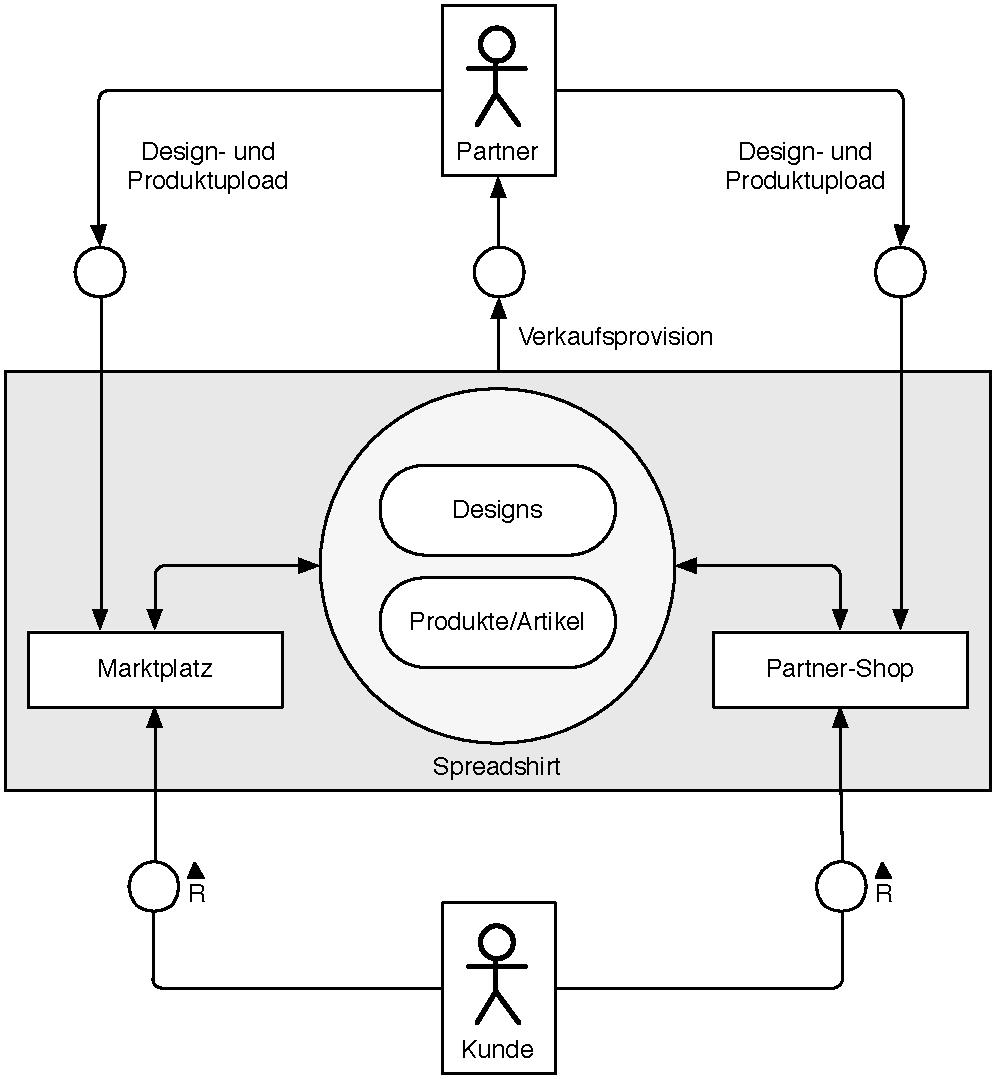
\includegraphics[width=0.65\textwidth]{how_spreadshirt_works}
\caption{FMC--Blockdiagramm der Spreadshirt--Bereiche und Benutzer}
\label{fig:howspreadshirtworks}
\end{figure}

Die grundsätzliche Funktionsweise der Spreadshirt--Plattform ist in \cref{fig:howspreadshirtworks} als FMC--Blockdiagramm dargestellt.

Das Suchergebnis für Suchen auf dem Marktplatz hängt maßgeblich von den Metadaten ab, die der Partner für seine Designs vergeben hat. Dazu gehören Tags, aber auch Titel und Beschreibung des Designs oder Produktes. In dieser Arbeit wird ausschließlich das Tagging--System betrachtet.

\label{platforms}
Spreadshirt betreibt aus historischen Gründen zwei Plattformen, deren Datenbestände größtenteils voneinander getrennt sind. Jeweils eine Plattform ist für den nordamerikanischen und den europäischen Markt zuständig. Im Kontext dieser Arbeit wird die europäische Plattform als Ausgangsbasis für alle Betrachtungen gewählt. Der Datenbestand dieser Plattform besteht aus circa 2 Millionen Tags, 6 Millionen Designs, 14 Millionen Produkten, 6 Millionen registrierten Nutzern und \num{750000} eröffneten Partner--Shops.

\subsection{Eigenschaften des Tagging--Systems}
\label{tag_sprd}

Im Fall von Spreadshirt ist die Vergabe von Tags auf die Menge der Partner \(P \subseteq U\) begrenzt (siehe auch \cref{spreadshirt}). Es handelt sich demnach um ein in \cref{tagging_types} beschriebenes teilweise geschlossenes Tagging--System.

Die Dokumente, die von den Partnern getaggt werden können, sind auf die Designs und Artikel beschränkt, die der Partner selbst angelegt hat. Eine Beschreibung kann somit ausschließlich durch den Autor des Inhaltes erfolgen. Deshalb fehlt im Vergleich zu anderen Tagging--Systemen auch die Information, welcher Benutzer den Tag vergeben hat, da diese implizit durch den Autor des Dokumentes gegeben ist.

Des Weiteren besitzen Tags in der Spreadshirt--Datenbank ein Attribut \emph{Sprache} aus der Menge \(L\). Die Sprache spielt bei der Eingabe und Anzeige der Tags zu Dokumenten eine Rolle. Je nach eingestellter Sprache auf der Website erstellt und sieht der Benutzer nur Tags, die mit dieser Sprache markiert sind.

Das Vokabular der Tags ist nicht eingeschränkt. Dies bringt zwangsläufig Probleme der Datenqualität mit sich, welche im folgenden Abschnitt erläutert werden.

\subsection{Datenqualität des Tagging--Systems}
\label{quality}

Die Qualität von Daten wird im Allgemeinen unter mehreren Gesichtspunkten beurteilt. Dazu gehören unter anderem \emph{Korrektheit}, \emph{Vollständigkeit}, und \emph{Redundanzfreiheit} \cite[S. 84 f.]{hkp2012}. Nachfolgend werden die bei Spreadshirt vorhandenen Tagging--Daten nach diesen Kriterien betrachtet und die Quellen eventueller Fehler \cite[S. 43 f.]{jo2003} diskutiert.

\subsubsection{Korrektheit}

Die Korrektheit der Tagging--Daten kann an vielen Punkten angezweifelt werden. Das hervorstechende Problem hierbei ist das Auftreten von Spam. Viele Partner versehen ihre Artikel und Designs mit Tags, die nicht den Inhalt beschreiben. Partner versehen ihre Designs und Artikel mit falschen Tags, damit diese bei populären Suchbegriffen gefunden werden.

Ein weiterer Defekt ist die Inkorrektheit des Attributes \emph{Sprache} der Tags. Die Sprache wird aus der Domain abgeleitet, die der Benutzer, der den Tag eingegeben hat, besucht hat. Viele Partner geben jedoch ihre Tags in mehreren Sprachen ein, um ihre Inhalte besser auffindbar zu machen. Dies führt in der Konsequenz dazu, dass das Attribut Sprache in einem nicht unwesentlichen Teil der Tags als falsch angesehen werden kann.

Die Quelle beider Fehler ist die bewusste Falscheingabe von Informationen, um einen persönlichen Vorteil zu erlangen, da die Partner versuchen, ihre Produkte möglichst zu vielen Sucheingaben in den Ergebnissen auftauchen zu lassen.
                                                                                                                                                                                                                                                                                                                                                                                                              
\subsubsection{Vollständigkeit}

Wie bereits in \cref{tag_sprd} beschrieben, fehlen in den Daten des Spreadshirt--Systems der Zeitpunkt und der Benutzer eines Taggings. Dies führt in der Konsequenz dazu, dass Spam schwerer erkannt werden kann. Zwar ist bekannt, wann ein Tag das erste Mal verwendet wurde, alle weiteren Verwendungen des Tags haben jedoch keinen Zeitstempel. Der Benutzer, der den Tag angelegt und verwendet hat, kann nur daraus abgeleitet werden, wer den getaggten Artikel angelegt hat.

Die Unvollständigkeit der Daten rührt in erster Linie daher, dass zum Zeitpunkt der Implementierung des Tagging--Systems noch nicht bedacht wurde, dass die fehlenden Attribute später nützlich sein können.

\subsubsection{Redundanzfreiheit}

Bedingt durch die Form der Dateneingabe besteht für das Vokabular des Tag--Systems ein großes Potential für redundante Daten. Da eingegebene Tags durch einen Separator getrennt eingegeben werden müssen, besteht hier Potential zur Fehleingabe. Wird der falsche Separator verwendet, werden die eigentlich getrennten Tags als eine einzige Entität abgespeichert.

Technisch kann jeder Tag genau ein Mal in der Datenbank vorkommen. Jedoch führen Tipp-- und Rechtschreibfehler, unterschiedliche Groß- und Kleinschreibung, verschiedene Arten zusammengesetzte Wörter zu schreiben, Leerräume vor, nach und zwischen Wörtern eines Tags und Tippfehler dazu, dass das gleiche Wort mehrfach in der Datenbank gespeichert wurde.

Außerdem führten in der Vergangenheit Systemfehler und Implementierungsfehler dazu, dass falsche, nicht druckbare Zeichen in den Tags enthalten waren. Nach Beseitigung der Fehler blieben die fehlerhaften Tags bestehen, so dass bei einer erneuten Eingabe des gleichen Wortes ein neuer Tag in der Datenbank angelegt wurde.

\subsection{Mengengerüst des Tagging--Systems}
\label{tag_amount}

Zum Zeitpunkt der Bearbeitung dieser Arbeit befanden sich im Datenbestand der europäischen Spreadshirt--Plattform:

\begin{itemize}
    \item \num{2072079} Tags in \num{15} verschiedenen Sprachen
    \item \num{6433410} Benutzer
    \item \num{26147860} Dokumente (\num{16494430} Artikel und \num{9653430} Designs)
    \item \num{71938905} Taggings
\end{itemize}

Diese Datenmengen stellen besondere Anforderungen an die Verarbeitung. Wie diese umgesetzt wurden, wird in \cref{system} diskutiert.

\section{Zusammenfassung}

Dieses Kapitel befasste sich mit Tagging--Systemen. Dazu wurden die Grundlagen und Begriffe genannt, die Vor-- und Nachteile von Tagging--System erläutert, das Datenmodell formalisiert und die grundsätzlichen Arten Folksonomy und teilweise geschlossenes Tagging--System unterschieden.

Außerdem wurde das im weiteren Verlauf dieser Arbeit verwendete Tagging--System von Spreadshirt \cite{sprd2013} näher betrachtet. Dazu wurden die speziellen Eigenschaften dieses Systems, die Datenqualität und die Menge der vorhandenen Daten beschrieben.

Das nachfolgende Kapitel beschäftigt sich mit dem zur Link Discovery angewandten Framework.
\chapter{Link--Discovery--Framework}
\label{ld_framework}

\emph{Link Discovery} \cite{na2011, vbgk2009}, oder \emph{Link Prediction} \cite{twak2003, nk2007}, bezeichnet Methoden des Data Minings \cite{hkp2012}, die zum Ziel haben, Verbindungen zwischen Objekten herzustellen. Diese Verbindungen werden aus vorhandenen Daten abgeleitet.

Das folgende Kapitel beschreibt das Framework, dass für die Link Discovery im Rahmen dieser Arbeit angewendet wurde. Das Framework beschreibt die Kombination aus dem modellierten Weltausschnitt, dem Prozess zur Herstellung der Beziehungen, Kookkurrenz als Maß für Beziehungen, Graphen als Mittel zur Beschreibung des Weltausschnittes, möglichen Datenquellen und evolutionären Algorithmen als Mittel zur Prioisierung der erzeugten Beziehungen.

\section{Modell des Weltausschnittes}
\label{world_model}

Der folgende Abschnitt beschäftigt sich mit der Modellierung des im Rahmen dieser Arbeit verwendeten Weltausschnittes. Das Entity--Relationship--Diagramm des resultierenden Modelles ist in \cref{fig:world_model} dargstellt.

\begin{figure}[t]
\centering
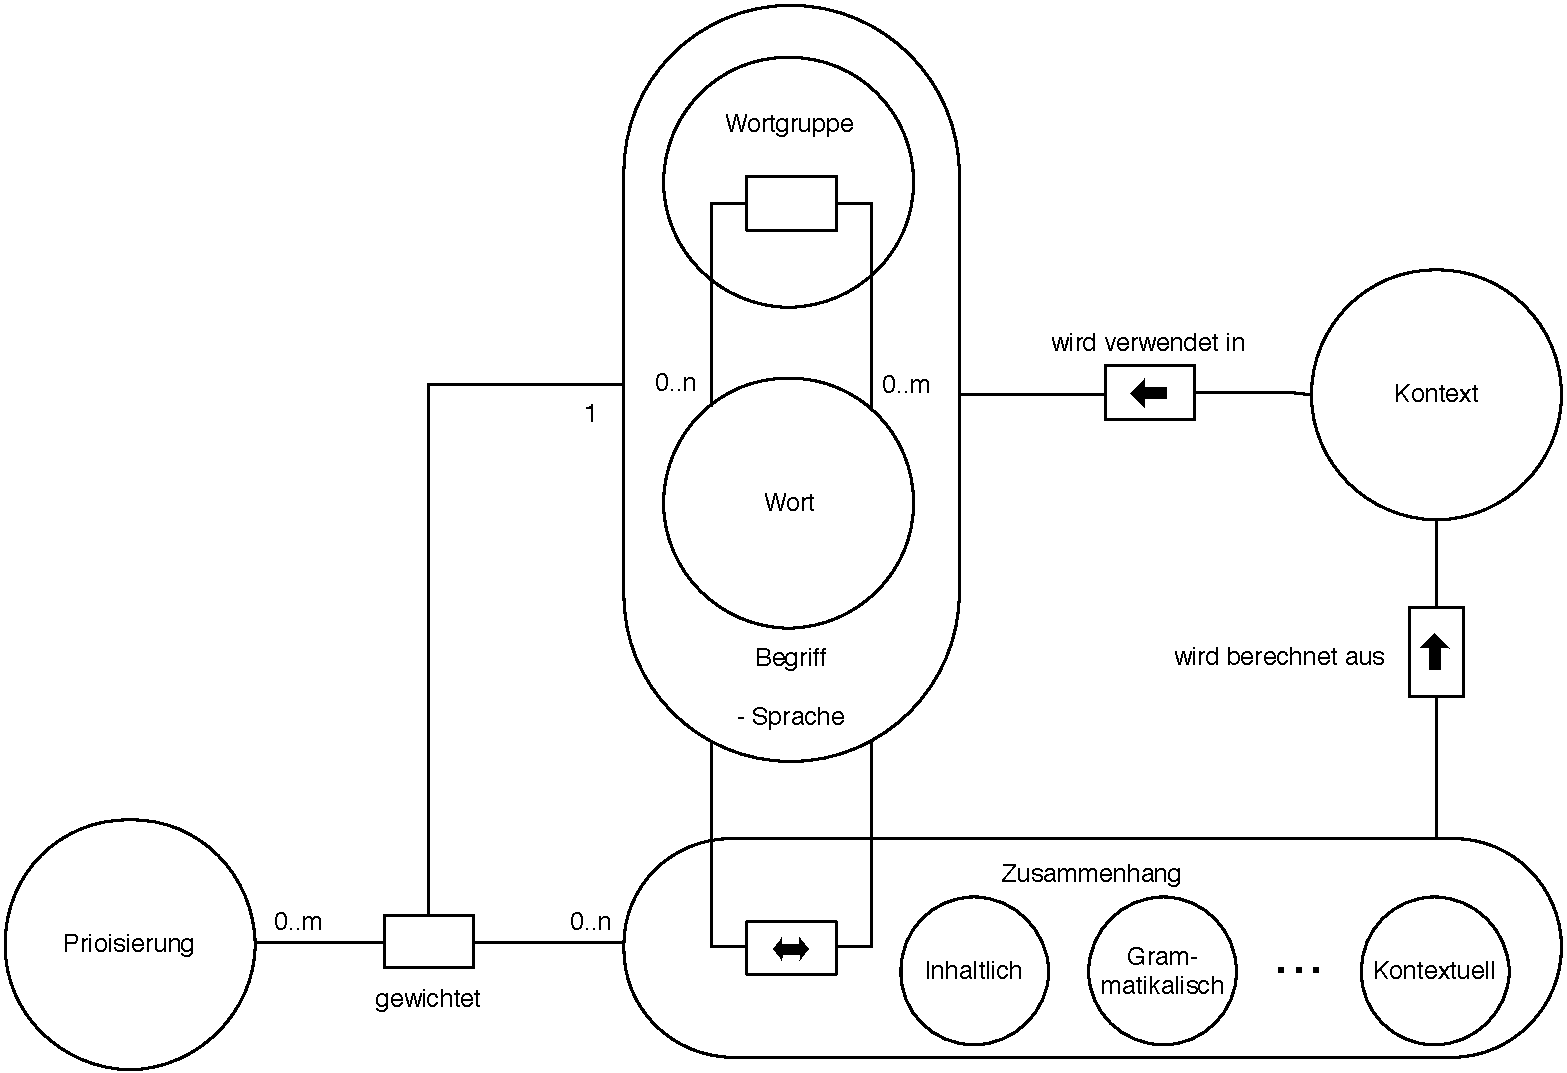
\includegraphics[width=\textwidth]{abstract_world_model}
\caption{FMC--Entity--Relationship--Diagramm des Modells des Weltausschnittes}
\label{fig:world_model}
\end{figure}

Zentrale Entität ist des Modells der \emph{Begriff}. Ein Begriff repräsentiert ein Einzelwort oder eine Wortgruppe in einer bestimmten Sprache. Dies berücksichtigt den Umstand, dass Wörter in mehreren Sprachen vorkommen können, jedoch in den jeweiligen Kulturräumen verschiedene Bedeutungen besitzen. Wortgruppen können aus beliebig vielen Einzelwörtern zusammengesetzt sein. Mit Hilfe der Link Discovery sollen zwischen diesen Begriffen verschiedenartige \emph{Zusammenhänge} gefunden werden.

Ein Zusammenhang (oder \emph{Beziehung}) besteht immer zwischen genau zwei Begriffen und besitzt einen bestimmten \emph{Typ}. Der Typ bezeichnet die Art des Zusammenhangs zwischen diesen beiden Begriffen. Beispiele für Zusammenhangstypen sind inhaltliche Zusammenhänge wie Synonyme, grammatikalische Zusammenhänge wie Wort-- und Grundformen oder kontextuelle Zusammenhänge, die sich aus der Verwendung des Begriffes ergeben. Dabei kann ein Zusammenhang abhängig vom Typ Attribute besitzen, die den Zusammenhang genauer spezifizieren. Dies kann beispielsweise ein Gewicht des Zusammenhangs sein, dass die Wichtigkeit gegenüber anderen Beziehungen gleichen Typs angibt.

Je nach Nutzungsform der Daten wird unter Umständen eine andere Sicht auf die Beziehungen benötigt. Eine \emph{Prioisierung} stellt eine Gewichtung der Beziehungen eines Begriffes nach Typ dar. Sie teilt jeder Zusammenhangsart ein Gewicht relativ zu den anderen Arten zu. Somit werden durch die Prioisierung bestimmte Zusammenhänge höher gewichtet als andere. Die Prioisierung wird zu einer auf den Anwendungsfall abgestimmten Ordnung der Beziehungen eines Begriffes genutzt.

Dies Verwendung eines Begriffes wird durch den \emph{Kontext} beschrieben. Dieser Kontext repräsentiert, wie der Begriff innerhalb einer bestimmten Anwendungsdomäne verwendet wurde. Daher sind die Attribute, die ein Kontext besitzen kann, nicht vorab spezifizierbar. Sie hängen von der jeweiligen Anwendungsdomäne ab. Beispiele für Kontexte sind die Verwendung eines Begriffes in einem Tag--System oder in einer Ontologie. Aus diesem Kontext werden im Laufe der Link Discovery Zusammenhänge berechnet.

Dieses Modell bildet die Grundlage für  im folgenden Abschnitt beschriebenen Link--Discovery--Prozess.

\section{Link--Discovery--Prozess}
\label{ld_process}

\begin{figure}[ht]
\centering
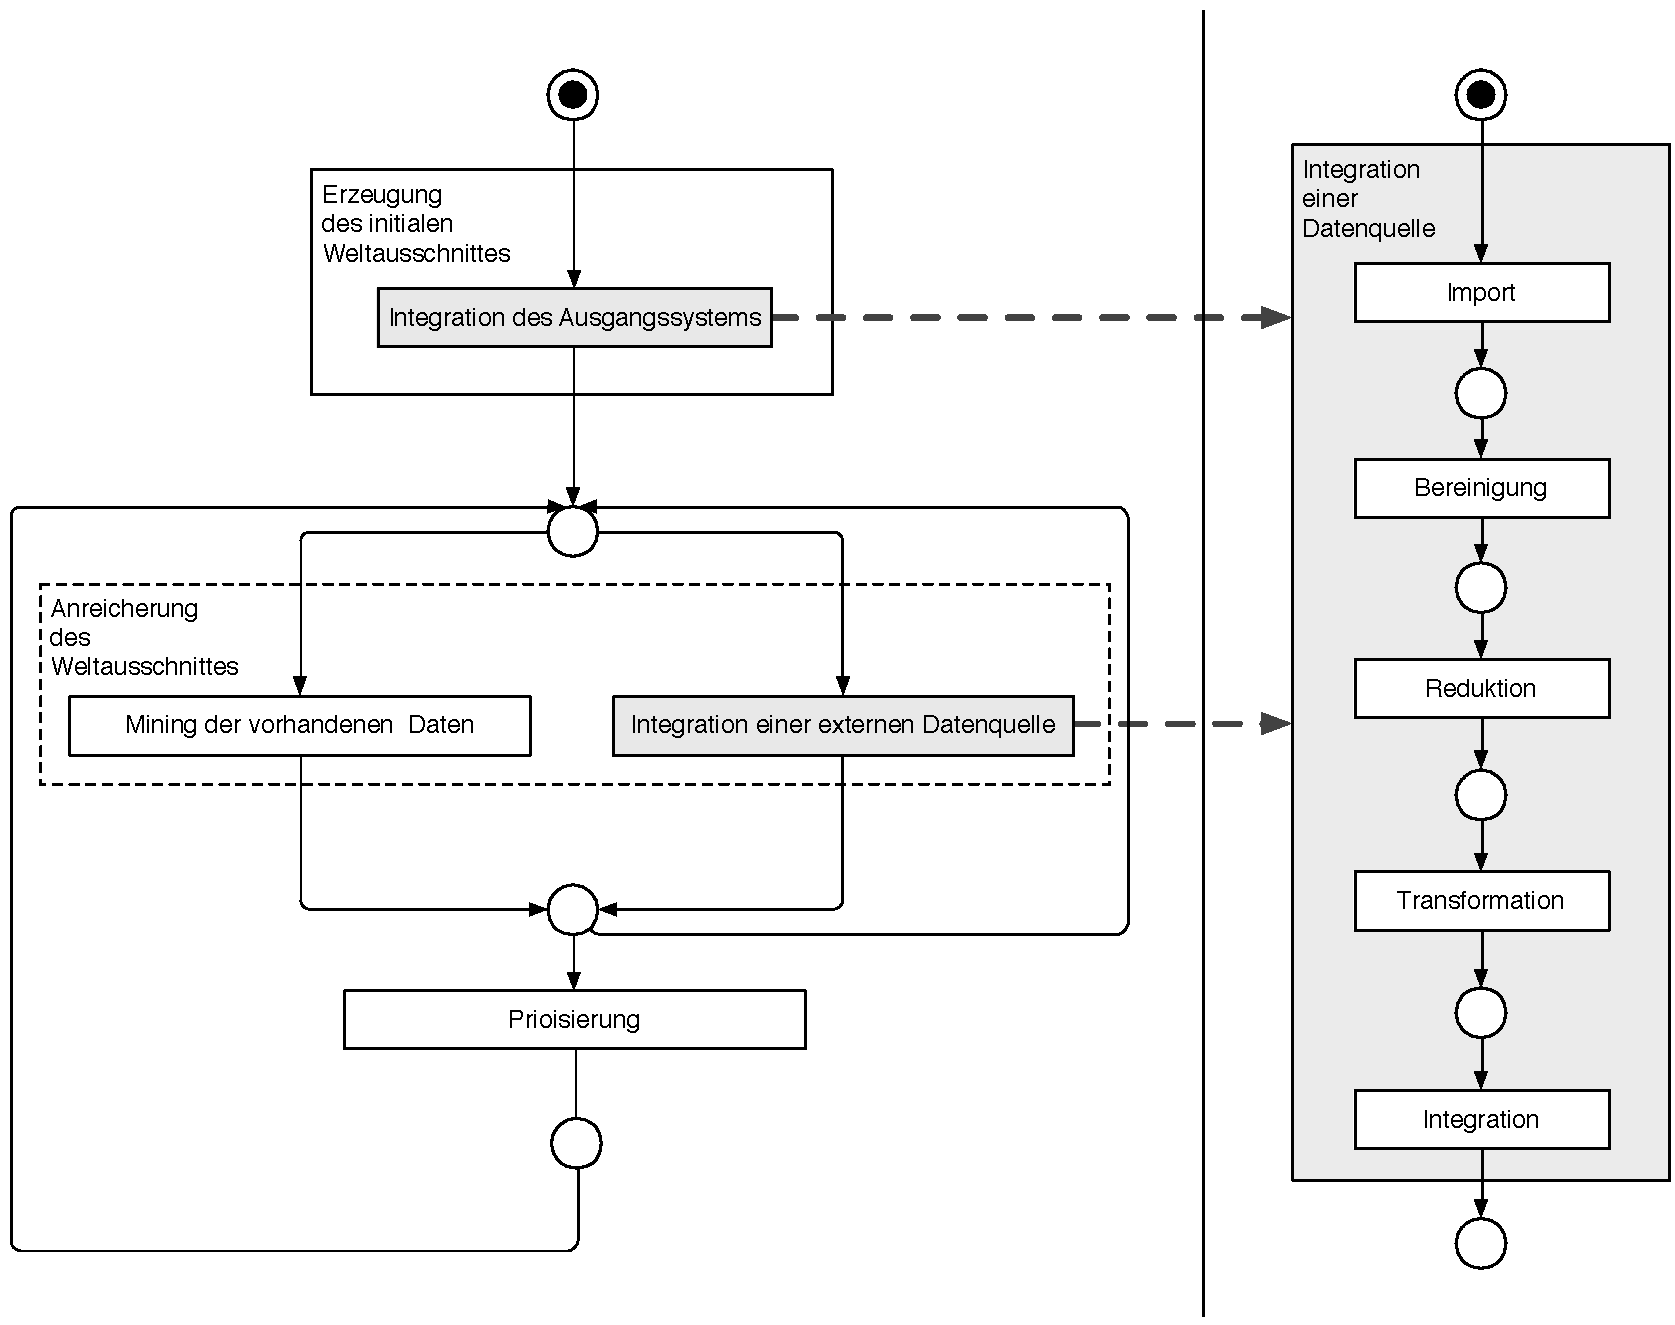
\includegraphics[width=\textwidth]{link_discovery_process}
\caption{FMC--Petri--Netz des Link--Discovery--Prozesses}
\label{fig:link_discovery_process}
\end{figure}

Der Link--Discovery--Prozess beschreibt die Abfolge von Schritten, die zur Erzeugung und Anreicherung des in \cref{world_model} beschriebenen Weltausschnittes angewendet werden. Dieser Prozess dient also zur Erzeugung von Begriffen und deren Zusammenhängen. \cref{fig:link_discovery_process} zeigt den Prozess als Petri--Netz.

Die grundlegenden Phasen des Prozesses sind die \emph{Erzeugung} des initialen Weltausschnittes, dessen \emph{Anreicherung} und die \emph{Prioisierung} der Beziehungen. Sowohl bei der initialen Erzeugung, als auch bei der Anreicherung wird ein Prozess zur Integration von Datenquellen benötigt.

Die Schritte der Anreicherung und Prioisierung können beliebig oft wiederholt werden, um das Ergebnis zu verbessern und auf die gewünschte Anwendung anzupassen. Die Anreicherung kann grundsätzlich durch das Mining der bereits im Weltausschnitt vorhandenen Daten oder durch die Integration neuer Datenquellen erfolgen.

Die genannten Schritte werden in den folgenden Abschnitten erläutert.

\subsection{Integration von Datenquellen}
\label{integration_generic}

Für die Link Discovery wird ein einheitliches Vorgehen zur Integration von Datenquellen benötigt. Die Datenquellen stellen grundsätzlich für die Link Discovery nützliche Daten zur Verfügung, die jedoch im Allgemeinen noch nicht direkt dem Modell des Weltausschnittes entsprechen. Demzufolge müssen diese Daten entsprechend verarbeitet werden.

Die zur Integration von externen Datenquellen nötigen Schritte entsprechen im Wesentlichen den von \textcite[S. 48f.]{hkp2012} beschriebenen Aufgaben der Datenvorverarbeitung: \emph{Bereinigung}, \emph{Reduktion}, \emph{Transformation} und \emph{Integration}. Diesen wird in dieser Arbeit der Schritt \emph{Import} vorangestellt, da es nicht immer möglich ist, den gesamten Datenbestand einer Datenquelle zu nutzen. Somit sollten im Importschritt auch die Anfragen an die Datenquelle spezifiziert werden. Die genannten Schritte werden zur Link Discovery immer in der genannten Reihenfolge ausgeführt und werden im folgenden kurz beschrieben.

\paragraph{Import}

Im Importschritt werden die Rohdaten aus der Datenquelle extrahiert. Dabei wird die Form der Daten nicht verändert. Ist es nicht möglich, den gesamten Datenbestand einer Quelle zu importieren, so muss eine Auswahl der anzufragenden Daten formuliert werden. Diese Auswahl richtet sich nach Möglichkeit nach den bereits im Weltausschnitt vorhandenen Daten. Beispielsweise können die Anfragen an die Datenquelle den bereits im Weltausschnitt gespeicherten Begriffen entsprechen.

\paragraph{Bereinigung}

Im nachfolgenden Bereinigungsschritt werden die importierten Daten so gut wie möglich von eventuell vorhandenen Defekten bezüglich der Datenqualität (siehe auch \cref{quality}) befreit. Dazu zählen beispielsweise das Entfernen nicht nutzbarer Zeichen oder von unvollständigen Datensätzen.

\paragraph{Reduktion}

Der Reduktionsschritt dient zur Verkleinerung der Datenmenge. Dazu gehören beispielsweise Schritte zur Duplikatentfernung oder zur Auswahl relevanter Datensätze. In dieser Arbeit bestand die Haupteinschränkung der Datenmenge darin, nach Möglichkeit nur deutschsprachige Begriffe auszuwählen.

\paragraph{Transformation}
\label{transformation}

Der Schritt der Transformation überführt die Daten schließlich in das Modell des Weltausschnittes. Dies bedeutet, dass die Datensätze in Begriffe und Beziehungen umgewandelt werden. Dabei sollten so viele Informationen über den Kontext der Begriffe erhalten bleiben. Die Methode, wie diese Transformation vorgenommen wird, hängt von der Datenquelle ab. Generell werden die Beziehungen meist aus dem Kontext der Begriffe, wie er in der Datenquelle vorliegt, gebildet. Ein Mittel für die Beziehungserzeugung ist die Kookkurrenz, welche in \cref{co-occurence} erläutert wird. Somit stellt der Transformationsschritt die wichtigste Komponente für die Integration einer Datenquelle dar.

\paragraph{Integration}

Der Integrationsschritt für jede Datenquelle dient letztendlich der Zusammenführung des im Transformationsschritt erzeugten Weltausschnittes mit dem bereits vorhandenen Weltausschnitt. Dabei werden bereits existierende Begriffe zusammengeführt und die neu erzeugten Beziehungen übernommen. Die Zusammenführung der Begriffe erfolgt über die Annotation des existierenden Begriffes mit dem neu erzeugten Kontext, den die Datenquelle zu einem Begriff liefert.

\subsection{Initiale Erzeugung des Weltausschnittes}

Der erste Schritt der Link Discovery besteht in der Auswahl einer geeigneten Datenquelle für die initiale Erzeugung des Weltausschnittes. In dieser Arbeit ist diese Datenquelle das Tagging--System von Spreadshirt (siehe \cref{tag_sprd}).

Die Auswahl der Datenquelle richtet sich im wesentlichen danach, ob der Kontext, den die Datenquelle potentiell zu Begriffen liefern kann, für die Link Discovery geeignet ist. Der Kontext sollte außerdem für die geplante Anwendung der Ergebnisse der Link Discovery relevant sein.

Nach der Auswahl einer geeigneten Quelle werden die in \cref{integration_generic} beschriebenen Schritte zur Integration durchgeführt. Der Schritt der Integration ist trivial, da zu diesem Zeitpunkt noch keine Daten im Weltausschnitt vorhanden sind.

\subsection{Anreicherung des Weltausschnittes}

Nach der initialen Erzeugung des Weltausschnittes kann dieser mit beliebig vielen Anreicherungsschritten ergänzt werden. Unter Anreicherung wird die Erzeugung neuer Begriffe, Kontexte oder Zusammenhänge verstanden.

Das Hinzufügen neuer Begriffe erweitert das Vokabular des Weltausschnittes. Somit können bei der Benutzung der Daten zu einer größeren Menge von Begriffen Zusammenhänge gefunden werden. Die Erzeugung von Kontexten zu vorhandenen oder neuen Begriffen erweitert das Wissen über die Benutzung eines Begriffes innerhalb einer bestimmten Anwendungsdomäne. Die Anreicherung des Weltausschnittes mit neuen Zusammenhängen ermöglicht einerseits das Finden von relevanten Nachbarn eines Begriffes, erfordert andererseits jedoch, abhängig von der Anwendung, auch eine andere Prioisierung der Zusammenhangstypen bei der Abfrage.

Grundsätzlich kann die Anreicherung des Weltausschnittes auf zwei Arten erfolgen. Dies ist zum die Anreicherung durch das Mining der bereits vorhandenen Daten, zum anderen die Anreicherung durch Integration einer weiteren Datenquelle.

\subsubsection{Anreicherung durch Mining vorhandener Daten}

Die Erzeugung neuer Begriffe und Zusammenhänge kann aus den vorhandenen Daten mittels Methoden des Data Minings vorgenommen werden. Dazu werden die bereits im Weltausschnitt vorhandenen Begriffe mit ihren Kontexten und Beziehungen analysiert, um bisher unbekannte Zusammenhänge zu finden.

Beispiele für anwendbare Methoden sind hierbei Assoziationsanalyse \cite[S. 328f.]{pt2013} oder Clusteranalyse \cite[S. 443f.]{hkp2012}, um bestimmte bereits in den Daten vorhandene, aber nicht explizit abgebildete, Zusammenhänge zu ermitteln. Jedoch können auch einfachere Methoden wie die Zerlegung von Wortgruppen in Einzelwörter (siehe \cref{decomposition}) oder das Einfügen von bisher nur transitiv, also nur über mehrere Begriffe, vorhandenen Beziehungen erfolgreich sein, um neue Begriffe und Beziehungen in den Datenbestand einzuführen.

\subsubsection{Anreicherung durch Integration externer Datenquellen}
\label{enrichment_external}

Sofern weitere Datenquellen verfügbar sind, stellt die Integration dieser einen weiteren erfolgversprechenden Weg dar, um die Daten anzureichern. Neue Datenquellen beschreiben immer einen neuen Kontext, in dem Begriffe genutzt werden. Ist der Kontext dieser Begriffe für die spätere Anwendung relevant, ist die Integration der jeweiligen Datenquelle zu Zwecken der Link Discovery von großem Interesse.

Um die zusätzliche Datenquelle zur Link Discovery zu nutzen, werden die Schritte, die schon zur initialen Erzeugung des Weltausschnittes zum Einsatz kamen, genutzt (siehe \cref{integration_generic}). Dazu werden im Transformationsschritt Daten erzeugt, die dem Modell des Weltausschnittes entsprechen. Im Integrationsschritt werden sie mit den bereits vorhandenen Daten zusammengeführt.

\subsection{Prioisierung von Beziehungen}
\label{prioritization}

Ziel des Prioisierungsschrittes der Link Discovery ist das Finden einer Gewichtung der Zusammenhangstypen, die für einen Anwendungsfall relevante Nachbarn zu einem Begriff liefert. Die Relevanz kann jedoch nur von einem Benutzer bewertet werden. \cref{fig:prioritization} stellt den Prioisierungsprozess dar.

\begin{figure}
\centering
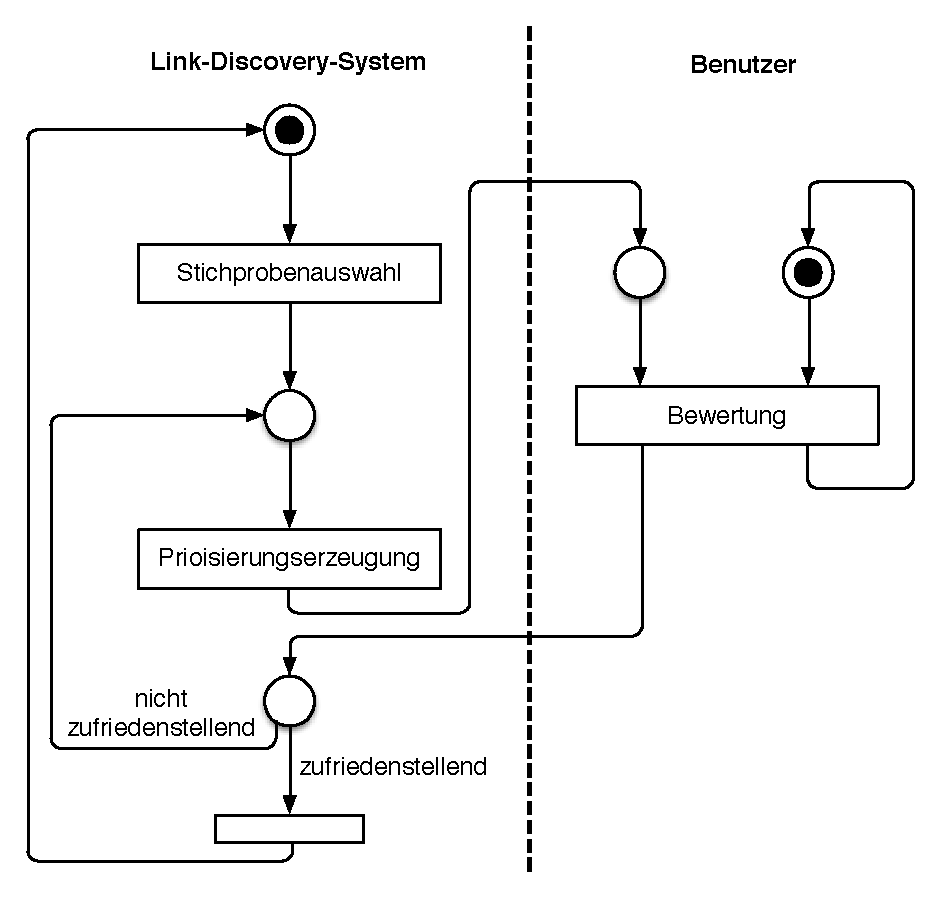
\includegraphics[width=0.7\textwidth]{prioritization}
\caption{FMC--Petri--Netz der Prioisierung}
\label{fig:prioritization}
\end{figure}

Grundsätzlich kann nicht davon ausgegangen werden, dass eine Prioisierung für alle im Weltausschnitt gespeicherten Begriffe relevante Nachbarn liefert. Daher sollte die Prioisierung stichprobenhaft für einzelne Begriffe durchgeführt werden, um dann möglicherweise eine global gute Ergebnisse liefernde Prioisierung zu ermitteln.

Der Prioisierungsprozess beginnt mit der Auswahl einer Stichprobe anhand geeigneter Kriterien für das Anwendungsszenario. Beispielhaft für Kriterien sind externe Faktoren wie die Popularität des Begriffes in der Anwendungsdomäne oder im Weltausschnitt gespeicherte Faktoren wie die Anzahl der Zusammenhänge, die ein Begriff besitzt. Wird der Prozess mit mehreren Stichproben durchgeführt, sollte auf eine möglichst breite Streuung des jeweiligen Kriteriums geachtet werden, um die Güte der Prioisierungen abhängig vom Begriff beurteilen zu können.

Nach der Auswahl der Stichprobe wird vom Link--Discovery--System eine Prioisierung erzeugt. Wie diese Erzeugung konkret implementiert ist, hängt von der Anwendung ab. Im Rahmen dieser Arbeit wurden Evolutionäre Algorithmen (siehe \cref{evo_for_prio}) gewählt. Die erzeugte Prioisierung wird auf den Begriff angewendet und von einem Benutzer bewertet. Der Benutzer sollte Wissen über die Anwendungsdomäne besitzen.

Ist die Bewertung der Prioisierung positiv, ist der Prioisierungsprozess beendet. Bei nicht zufriedenstellendem Ergebnis wird die Erzeugung einer neuen Prioisierung und die anschließende Bewertung wiederholt. Stellt sich auch nach einer im Voraus gewählten Anzahl von Iterationen dieser Art kein zufriedendstellendes Ergebnis ein, so sollte die Prioisierung abgebrochen werden und die Gründe für das Fehlschlagen analysiert werden. Diese können beispielsweise in einer schlechten Qualität der Beziehungen des Weltausschnittes, in einer unpassenden Stichprobenauswahl oder fehlendem Wissen des Benutzers gefunden werden.

\section{Kookkurrenz als Mittel zur Beziehungserzeugung}
\label{co-occurence}

Im Transformationsschritt der Link Discovery (\cref{transformation}) wird eine Methode benötigt, aus dem Kontext von Begriffen Beziehungen zwischen eben jenen zu berechnen. Eine der möglichen Methoden ist die Berechnung von \emph{Kookkurrenz}. Diese wird im folgenden Abschnitt näher erläutert.

\subsection{Grundlagen von Kookkurrenz}

Um gewichtete inhaltliche Beziehungen zwischen Begriffen herstellen zu können, wird eine Definition von \emph{Ähnlichkeit} benötigt. Diese lässt sich auf vielfältige Arten bestimmen.

\begin{figure}[h]
\centering
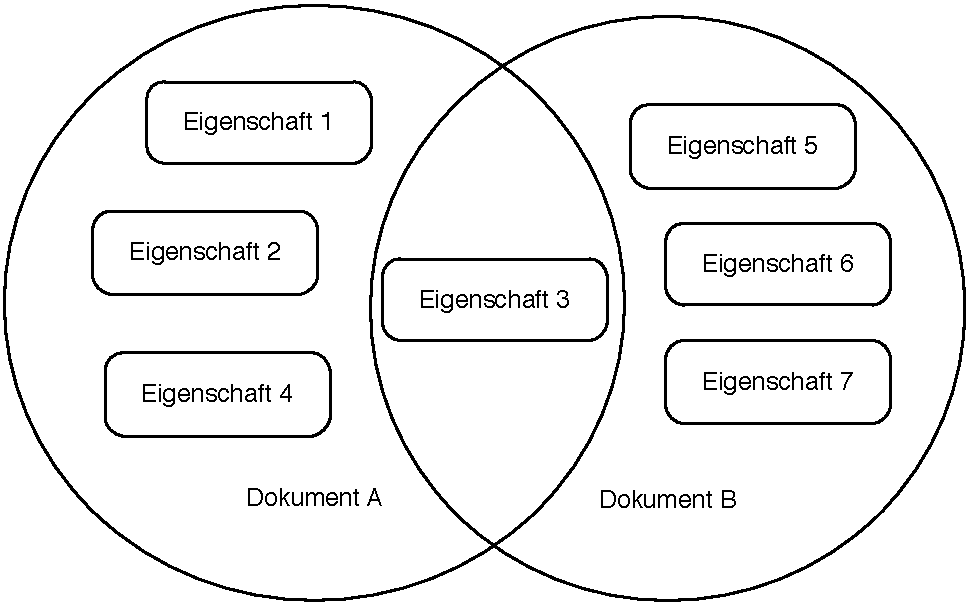
\includegraphics[width=0.6\textwidth]{similarity}
\caption{Repräsentation von Dokumenten als Mengen von Eigenschaften}
\label{fig:similarity}
\end{figure}

Die Ähnlichkeit zwischen zwei Dokumenten kann grundsätzlich nach \textcite{at1977} definiert werden. Dieser Definition liegt zu Grunde, dass sich die Dokumente als Mengen von Eigenschaften beschreiben lassen. Im Gegensatz zu anderen Ähnlichkeitsmodellen hängt die Ähnlichkeit nicht nur von den gemeinsamen Eigenschaften der Dokumente ab, sondern auch von den Eigenschaften, die die Dokumente allein besitzen. Diese Definition von Ähnlichkeit wird in \cref{fig:similarity} veranschaulicht.

Somit lässt sich Ähnlichkeit \(s(A,B)\) zwischen den Dokumenten, die durch die Mengen \(A\) und \(B\) dargestellt werden, definieren durch
\[s(A,B) = F(A \cap B, A-B, B-A)\]
\label{similarity}

Die Gestaltung der Funktion \(s\) und die Auswahl der für die Ähnlichkeitsberechnung genutzten Eigenschaften der Dokumente hängt stark von der Anwendung ab. Somit beschreibt beispielsweise die Levenshtein--Distanz \cite{vl1966} die Ähnlichkeit zweier Zeichenketten durch die minimale Menge von Einfüge-, Lösch- und Ersetzungsoperationen, die nötig sind, um eine Zeichenkette in die andere umzuwandeln. In Ontologien und Taxonomien kann die Ähnlichkeit von Begriffen mittels der Knoten- oder Kanteneigenschaften berechnet werden. Beispiele hierfür sind die Ähnlichkeit in Ontologien nach \textcite{pr1995} und \textcite{ps2002}. In der Bildverarbeitung können merkmalsbasierte Ähnlichkeitsmaße ebenfalls eingesetzt werden, beispielsweise beschreiben \textcite{ow2006} ein Ähnlichkeitsmaß auf Basis von Clusteringalgorithmen, die auf Rastergrafiken angewandt werden.

Im Rahmen dieser Arbeit wird ein Ähnlichkeitsmaß gesucht, dass anhand der Eigenschaften von Begriffen eine Distanz zwischen eben jenen berechnet. Da eine inhaltliche Ähnlichkeit gesucht wird, spielen linguistische Ähnlichkeitsmaße wie die Levenshtein--Distanz eine untergeordnete Rolle. Zu Beginn bestehen keinerlei Verbindungen zwischen den Begriffen, so dass keine Ähnlichkeitsmaße für Ontologien eingesetzt werden können. Somit bietet sich die Wahl eines Ähnlichkeitsmaßes an, das den Kontext, in dem die Begriffe im Quellsystem verwendet werden, berücksichtigt.

In \cref{tag_sprd} wurde das für diese Arbeit verfügbare Tagging--System beschrieben. In diesem System besitzen die Tags wenig Kontext. Die einzig verfügbare Information ist, an welche Dokumente die Tags vergeben wurden.

Wenn mehrere Begriffe pro Dokument verwendet werden, wird damit ein Zusammenhang zwischen den Begriffen beschrieben. Dieser Zusammenhang lässt sich mit dem Ähnlichkeitsmaß \emph{Kookkurrenz} messen. Kookkurrenzmaße beschreiben, wie oft Begriffe gemeinsam verwendet werden \cite[S. 21]{zz2011}. Dies wird ins Verhältnis zum einzelnen Auftreten der Begriffe gesetzt und genügt somit der Definition von Ähnlichkeit in \cref{similarity}.

Hierzu muss angemerkt werden, dass die Ähnlichkeit mittels Kookkurrenz nicht zwingend eine Ähnlichkeit der den Begriffen zu Grunde liegenden Konzepte darstellt. Die Verwendung von Kookkurrenz als Ähnlichkeitsmaß beruht allein auf der Annahme, dass Menschen zur Beschreibung von gleichen Inhalten die gleichen Begriffe benutzen. Diese Annahme muss im Laufe der Evaluierung der Ergebnisse validiert werden.

\subsection{Kookkurrenzmaße}
\label{measures}

Werden die Objekte, zwischen denen die Ähnlichkeit berechnet werden soll, als Mengen von Eigenschaften definiert, bieten sich die üblichen Kennzahlen für die Ähnlichkeiten von Mengen an. Ein Begriff kann also als Menge der Dokumente, für die er als Beschreibung verwendet wurde, definiert werden.

Um die Ähnlichkeit zwischen zwei Begriffen zu ermitteln, lassen sich die Vereinigungsmenge, Schnittmenge und Kreuzprodukte der jeweiligen Mengen bilden, die die Begriffe repräsentieren. Ist also \(A\) die Menge der Dokumente, die mit einem Begriff \(a\) versehen wurden, \(B\) die Menge der Dokumente mit einem Begriff \(b\), so ergeben sich die Mengen:

\begin{itemize}
    \item \(A \cap B\), alle Dokumente die mit \(a\) und \(b\) versehen wurden
    \item \(A \cup B\), alle Dokumente die mit \(a\) oder \(b\) versehen wurden
    \item \(A \times B\), alle Dokumentenpaare, die sich aus den Mengen \(A\) und \(B\) bilden lassen
\end{itemize}

Die Mächtigkeiten dieser Mengen können dann zur Berechnung verschiedener Ähnlichkeitsmaße verwendet werden. Drei der üblichsten Maße wurden im Rahmen dieser Arbeit verwendet und werden im Folgenden genannt.

\subsubsection{Sørensen--Dice}

Der Sørensen--Dice--Koeffizient \cite{st1948} \cite{ld1945}, oft auch nur Dice--Koeffizient, entstand ursprünglich in der Biologie und wurde verwendet, um die Ähnlichkeit zwischen Proben zu berechnen. Heute findet er allgemeine Anwendung im Data Mining. Er ist definiert durch:

\[
\delta_{Dice}(a, b) = \frac{2|A \cap B|}{|A|+|B|}
\]

Der Wertebereich des Koeffizienten liegt zwischen \num{0} und \num{1}.

\subsubsection{Jaccard}

Der Jaccard--Index \cite{pj19012} wurde ursprünglich mit dem gleichen Zweck wie der Dice--Koeffizient verwendet. Sein Wertebereich liegt ebenfalls zwischen \num{0} und \num{1} und er ist definiert durch:

\[
\delta_{Jaccard}(a,b) = \frac{|A \cap B|}{|A \cup B|}
\]

\subsubsection{Kosinus}

Die Kosinus-Ähnlichkeit \cite{hkp2012} ist ursprünglich ein Maß für die Ähnlichkeit zweier Vektoren. Sie ist eine Maßzahl dafür, ob die Vektoren ungefähr in die gleiche Richtung zeigen. Sie kann jedoch genauso auf Mengen angewendet werden, da das Vorhandensein der Elemente in der Menge auch durch einen Vektor in einem \(n\)-dimensionalen Raum dargestellt werden kann, wobei \(n\) die Anzahl aller möglichen Eigenschaften ist. Der Wertebereich der Kosinus-Ähnlichkeit liegt ebenfalls zwischen \num{0} und \num{1}. Sie ist auf den in \cref{measures} definierten Mengen definiert durch:

\[
\delta_{Cosine}(a, b) = \frac{|A \cap B|}{\sqrt{|A| \times |B|}}
\]

Nachdem die Ähnlichkeit mittels Kookkurrenz und die entsprechenden Maße vorgestellt wurden, wird im nächsten Abschnitt die Berechnung und damit verbundene Komplexität diskutiert.

\subsection{Berechnung von Kookkurrenz}

Um die in \cref{measures} genannten Maße für Kookkurrenz zu berechnen, muss das Kreuzprodukt aller Begriffe gebildet werden. Dabei muss für jedes Paar von Begriffen die Häufigkeit gezählt werden, wie oft die Begriffe gemeinsam zur Beschreibung von Dokumenten verwendet wurden. Diese Häufigkeit beschreibt die Mächtigkeit der Mengen \(A \cap B\). Außerdem muss gezählt werden, wie oft jeder Begriff insgesamt verwendet wird, um die Mächtigkeit der Mengen \(A, B, \dots\) zu bestimmen. Danach können über die genannten Formeln die Kookkurrenzmaße berechnet werden. In \cref{lst:coocc-pseudo} ist die Berechnung als Pseudo--Code dargestellt.

\begin{lstlisting}[language=pseudo, label={lst:coocc-pseudo}, caption={Kookkurrenzberechnung}]
var occurences = {};

foreach (term in terms) {
    occurences[term] = countOccurrences(term);
}

foreach (termA in terms) {
    foreach (termB in terms) {
        ab = countCoOccurences(termA, termB);
    }
    dice = dice(occurences[termA], occurences[termB], ab);
    jaccard = jaccard(occurences[termA], occurences[termB], ab);
    cosine = cosine(occurences[termA], occurences[termB], ab);
}
\end{lstlisting}

Der Aufwand, um die Kookkurrenzmaße für alle Paare von Begriffen zu berechnen, hängt also von der Anzahl der Begriffe, Dokumente und Verwendungen ab. Beträgt die Anzahl der Begriffe \(n\) und die Anzahl der Dokumente \(d\), so ergibt sich für den Fall, dass jeder Begriff an jedes Dokument vergeben wurde eine Laufzeit von \(O(d*n^2)\). Wurden keine Begriffe mit Dokumenten verknüpft, beträgt die Laufzeit \(\Theta(d)\). Die reale Laufzeit der Ähnlichkeitsberechnung liegt daher zwischen diesen Schranken.

Es ist also absehbar, dass der Rechenaufwand mit wachsender Datenmenge stark ansteigt. Somit scheint es ratsam, nach Optimierungen zu suchen, um die Rechenzeit zu verringern. Da sich die Anzahl der Berechnungen nicht vermindern lässt, kann eine Verkürzung der Rechenzeit nur durch Parallelisierung erreicht werden. Eine mögliche Umsetzung der parallelen Berechnung der Kookkurrenz mittels des Programmiermodelles  MapReduce wird in \cref{mapreduce_cooccurence} erläutert.

\section{Graphen als Beschreibungsmittel des Weltausschnittes}

Nachdem in \cref{world_model} der zur Link Discovery verwendete Weltausschnitt modelliert wurde, wird zur Umsetzung eine Datenstruktur benötigt, die diesen Ausschnitt konkret abbildet. Da im Wesentlichen Objekte, zwischen denen Verbindungen bestehen, abgebildet werden, bietet sich die Verwendung eines Graphen an. Die Grundlagen von Graphen, sowie die konkrete Abbildung des Weltausschnittes auf eine Graph--Datenstruktur werden in den folgenden Abschnitten erläutert.

\subsection{Grundlagen}
\label{graph_basics}

Ein \emph{ungerichteter Graph} ist definiert durch ein Paar \(G = (V,E)\) von Mengen, für die gilt: \(E \subseteq\ [V]^2\). Dies bedeutet, dass alle Elemente aus \(E\) 2-elementige Teilmengen von \(V\) sind \cite[S. 2]{rd2012}. Die Menge \(V\) repräsentiert die \emph{Knoten} und die Menge \(E\) die \emph{Kanten} des Graphen. Eine Kante stellt eine Verbindung von zwei Knoten dar. Zwei Knoten werden als \emph{Nachbarn} bezeichnet, wenn zwischen ihnen eine Kante existiert. \cref{fig:basic_graph} zeigt ein Beispiel für einen ungerichteten Graphen.

\begin{figure}[h]
\centering
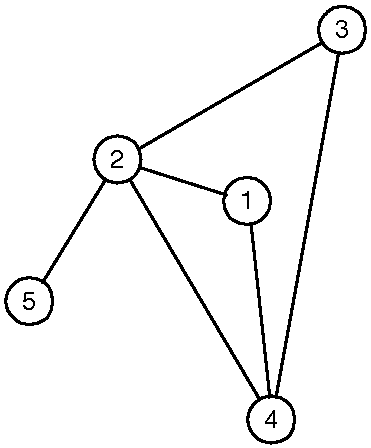
\includegraphics[width=0.2\textwidth]{basic_graph}
\caption{Ungerichteter Graph}
\label{fig:basic_graph}
\end{figure}

Ein \emph{gerichteter Graph} ist ein Graph, der neben den Mengen \(V\) und \(E\) die zwei Abbildungen \(quelle: E \rightarrow V\) und \(ziel: E \rightarrow V\) enthält \cite[S. 25]{rd2012}. Diese weisen jeder Kante \(e\) einen Quell- und Zielknoten zu. Die Kante ist somit von \(quelle(e)\) nach \(ziel(e)\) gerichtet. \cref{fig:directed_graph} zeigt einen gerichteten Graphen.

\begin{figure}[ht]
\centering
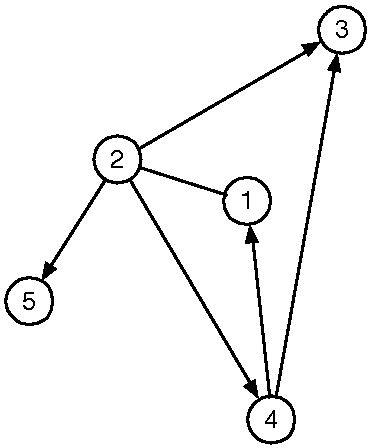
\includegraphics[width=0.2\textwidth]{directed_graph}
\caption{Gerichteter Graph}
\label{fig:directed_graph}
\end{figure}

Als \emph{Multigraph} wird schließlich ein Graph bezeichnet, bei dem zwischen zwei Knoten mehrere Kanten bestehen \cite[S. 25]{rd2012}. Sind diese gerichtet, spricht man vom einen \emph{gerichteten Multigraph}. \cref{fig:directed_multigraph} illustriert einen solchen gerichteten Multigraph.

\begin{figure}[h]
\centering
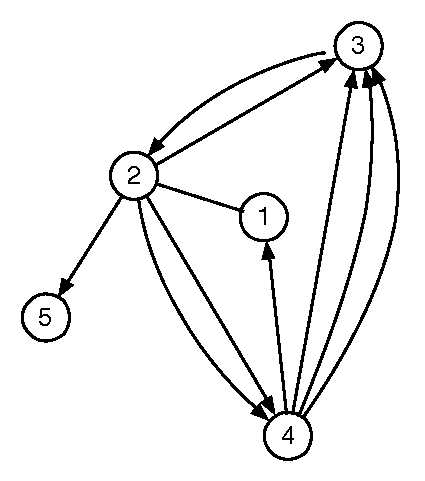
\includegraphics[width=0.2\textwidth]{directed_multigraph}
\caption{Gerichteter Multigraph}
\label{fig:directed_multigraph}
\end{figure}

Die Knoten und Kanten eines Graphen sind Objekte mit beliebigen weiteren Eigenschaften. Kanten besitzen üblicherweise ein Gewicht, dass ihre Wichtigkeit oder Kosten im Anwendungskontext des Graphen angibt.

Nachdem Graphen grundsätzlich erläutert wurden, beschäftigt sich der folgende Abschnitt mit der konkreten Umsetzung des Modelles des Weltausschnittes auf eine solche Graphen--Struktur.

\subsection{Graphenrepräsentation des Weltausschnittes}

Um den Weltausschnitt in \cref{world_model} in eine Graphenform zur transformieren, muss zunächst modelliert werden, welche Objekte die Knoten und Kanten des Graphen repräsentieren.

\begin{figure}
\centering
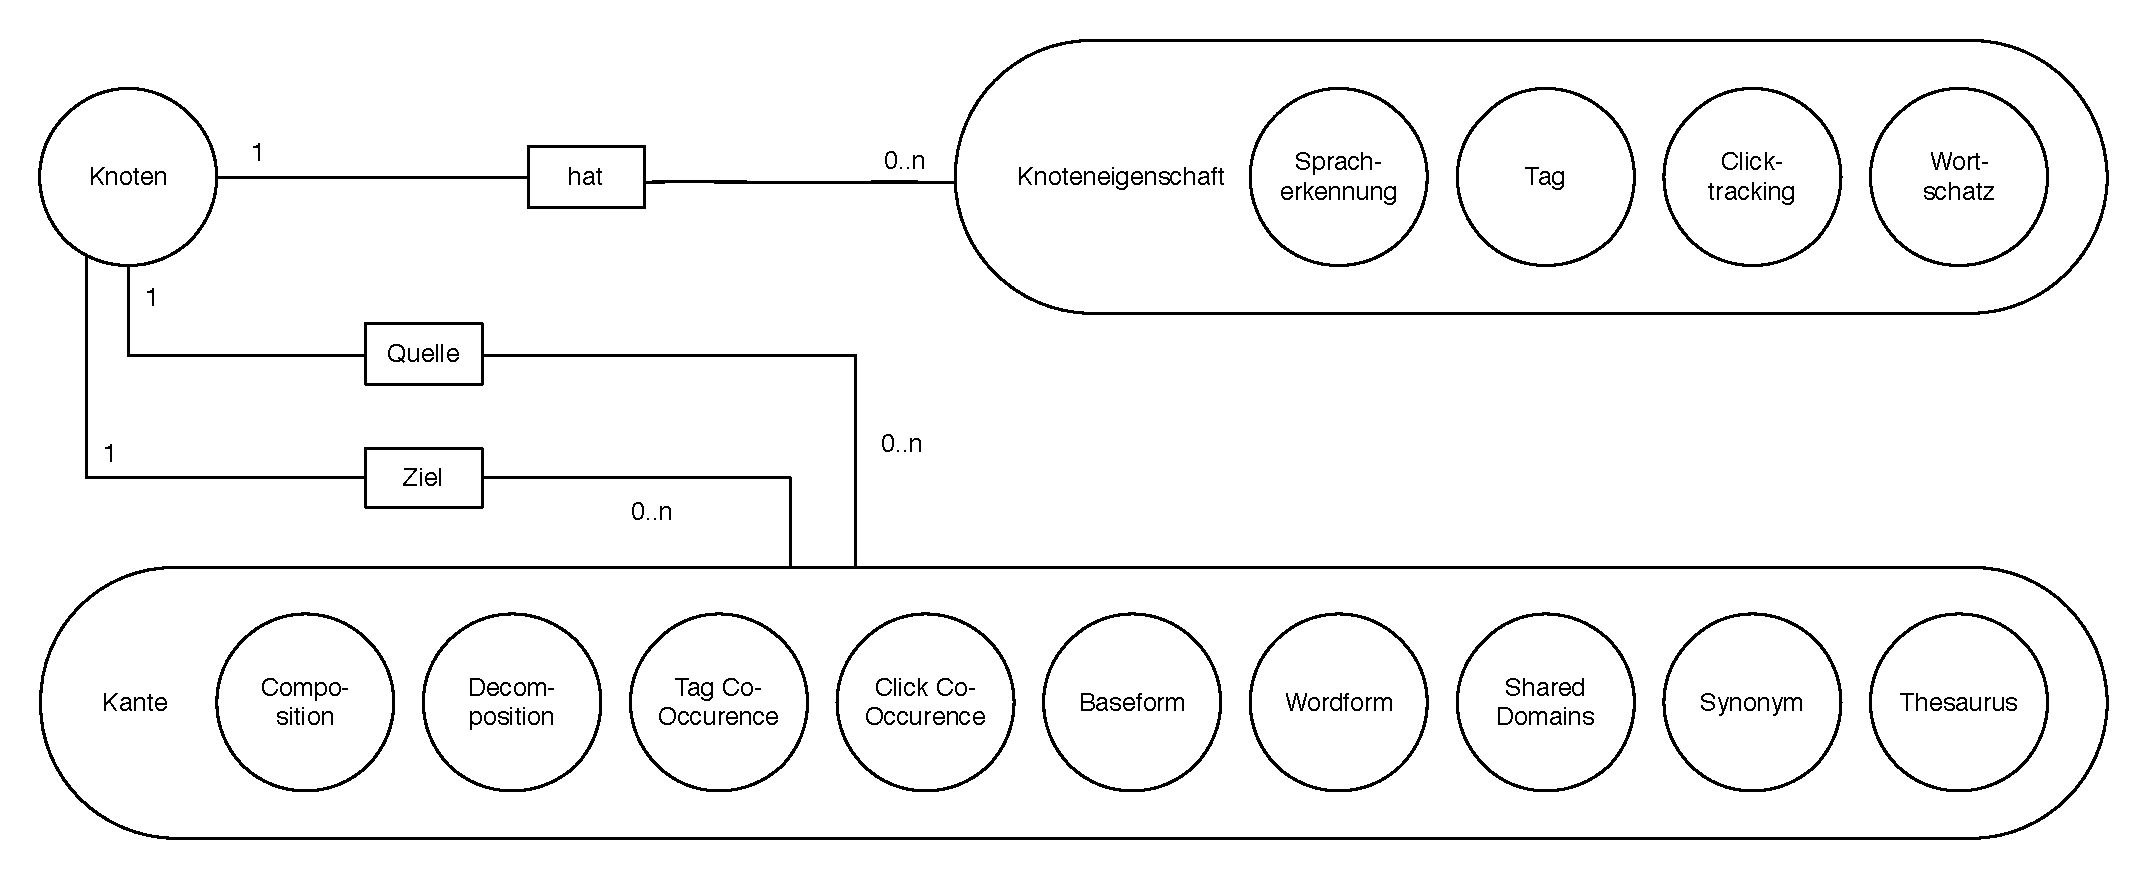
\includegraphics[width=1\textwidth]{graph_model}
\caption{FMC--Entity--Relationship--Diagramm der Graphenrepräsentation}
\label{fig:graph_model}
\end{figure}

Die Knoten repräsentieren die Begriffe, zwischen denen durch die Link Discovery Zusammenhänge hergestellt werden sollen. Sie enthalten als benötigte Attribute eine Zeichenkette und ein Attribut Sprache. Die Kombination dieser beiden Attribute ist innerhalb der Knotenmenge eindeutig, um je verwendetem Begriff in einer Sprache genau einen Knoten zu erhalten.

Der Kontext der Begriffe wird über Eigenschaften von Knoten abgebildet. Dabei kann ein Begriff beliebig viele Eigenschaften besitzen. Da die Kontexte der Begriffe aus jeweils einer Datenquelle stammen, bietet es sich an, pro Datenquelle eine Entität für die kontextuellen Eigenschaften, die diese Datenquelle liefert, zu definieren.

Eine Kante repräsentiert einen irgendwie gearteten Zusammenhang zwischen zwei Begriffen. Sie besitzt einen \emph{Typ}, der die Art des Zusammenhangs spezifiziert, sowie je einen Quell- und Zielknoten. Zusätzlich kann sie weitere Attribute besitzen. Bei Kanten, die durch Kookkurrenzberechnung (siehe \cref{co-occurence}) erzeugt wurden, sind dies beispielsweise die Anzahl des gemeinsamen Auftretens zweier Begriffe und die berechneten Kookkurrenzmaße. Im Rahmen dieser Arbeit wurden keine weiteren Attribute für Kanten benötigt, diese sind generell jedoch denkbar.

Zwischen zwei Knoten können beliebig viele, je Typ jedoch höchstens eine, Kanten existieren. Daher handelt es sich bei dem Graphen des Weltausschnittes um einen gerichteten Multigraph (siehe \cref{graph_basics}).

Das resultierende komplette Modell des Graphen ist in \cref{fig:graph_model} dargestellt. Dieses beinhaltet sämtliche zum Zeitpunkt der Bearbeitung bekannten und integrierten Datenquellen und die damit verbundenen Kontexte und Kantentypen. Die Datenquelle des Tagging-Systems und der damit verbundene Kontext wird in \cref{tag_sprd} näher beschrieben. Das Clicktracking--System wird in \cref{clicktracking} und der Wortschatz der Universität Leipzig in \cref{wortschatz} näher beleuchtet. Details über die Erzeugung der entsprechenden Kantentypen werden in \cref{link_discovery} erläutert.

\begin{figure}[t]
\centering
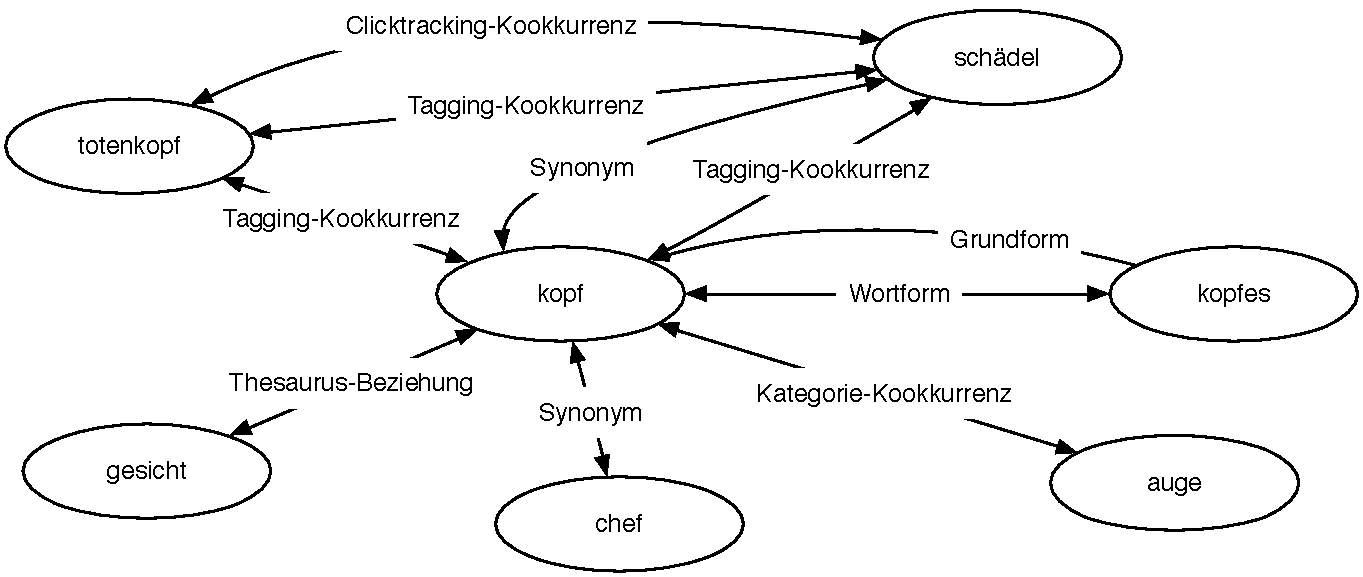
\includegraphics[width=\textwidth]{example_graph}
\caption{Beispiel--Graphausschnitt für das Ergebnis der Link Discovery}
\label{fig:example_graph}
\end{figure}

Um die Graphenrepräsentation des modellierten Weltausschnittes anschaulicher darzustellen, ist in \cref{fig:example_graph} ein beispielhafter Ausschnitt des nach Durchführung der Link Discovery entstehenden Graphen abgebildet. Auf Darstellung der Kontexte und Kantenattribute wurde aus Platzgründen verzichtet.

Nach der Definition der verwendeten Graphenstruktur werden im folgenden Abschnitt die möglichen Datenquellen diskutiert.

\section{Datenquellen zur Anreicherung}

Der initiale Weltausschnitt wird im Rahmen dieser Arbeit aus den Daten des Tagging--Systems von Spreadshirt erzeugt. Wie in \cref{enrichment_external} bereits einführend erläutert, kann danach zur Anreicherung die Integration weiterer Datenquellen erfolgen. Diese Datenquellen können eine andere Sicht auf die Begriffe des Weltausschnittes liefern und somit zur Erzeugung neuer Beziehungen nützlich sein. In diesem Abschnitt werden mögliche Datenquellen genannt und erläutert, sowie die letztendlich verwendeten Datenquellen näher beschrieben.

\subsection{Lexikalische Quellen}

Da die Hauptentität des Weltausschnittes Begriffe einer Sprache darstellt, liegt nahe, auf lexikalische Quellen zurückzugreifen. Diese existieren in unterschiedlichen Ausprägungen, haben jedoch alle gemeinsam, dass sie Wörter beschreiben und in Beziehung zu anderen Wörtern setzen. Damit eignen sie sich gut zur Integration in den Weltausschnitt. Einige der üblichen Formen von lexikalischen Quellen werden im folgenden genannt und erläutert.

Ein \emph{Wörterbuch} ist ein Nachschlagewerk, dass erklärende Informationen über Wörter enthält \cite{hk2003}. Dabei kann es sich um Sach- oder Sprachwissen handeln, also einerseits die inhaltliche Bedeutung eines Wortes oder andererseits die linguistischen und grammatikalischen Eigenschaften des Wortes beschreiben. Beispiele für Wörterbücher sind der \emph{Duden} \cite{duden} oder das \emph{Oxford English Dictionary} \cite{oed2010}.

Als \emph{Thesaurus} wird ein kontrolliertes Vokabular von Wörtern bezeichnet, die nach ihrer inhaltlichen Bedeutung geordnet sind \cite[S. 2]{ac2004}. Er stellt demnach eine Sammlung von \emph{Synonymen}, also Wörtern mit gleicher Bedeutung, dar und enthält keine Definitionen der Wörter. Oft enthalten Thesauri ebenfalls Ober- und Unterbegriffe und beschreiben somit \emph{Taxonomien}. Beispiele für Thesauri sind OpenThesaurus \cite{ot2013} für die deutsche und Thesaurus.com \cite{tc2013} für die englische Sprache. Thesauri sind eine spezielle Form von Wörterbüchern.

\emph{Wortschätze} sind eine Mischform aus Sprach- und Sachwörterbüchern. Sie enthalten zu möglichst vielen im Gebrauch befindlichen Wörtern einer Sprache Informationen über Verwendung, Bedeutung, Über- und Unterbegriffe, grammatikalische Eigenschaften und mehr.
Für die englische Sprache existiert die \emph{WordNet}--Datenbank \cite{wn2013, fc1998}, die Synonyme, Wortformen, Bedeutungen, Über- und Unterbegriffe, Beispiele und mehr für englische Wörter katalogisiert. Für die deutsche Sprache betreibt die Universität Leipzig mit dem \emph{Deutschen Wortschatz} ein ähnliches Projekt \cite{ws2013}.

Generell sind lexikalische Quellen also geeignet, um den Weltausschnitt mit Allgemeinwissen über die enthaltenen Begriffe anzureichern. Sie bieten allgemeine Informationen über Wörter und sind somit in vielen Anwendungsszenarien nutzbar.

\subsection{Clicktracking--System}

Die Aufgabe eines \emph{Clicktracking--Systems} besteht im Wesentlichen darin, die Klicks auf Hyperlinks von Benutzern einer Website aufzuzeichnen. Dabei wird für gewöhnlich auch aufgezeichnet, in welchem Kontext der Klick statt fand. Der Kontext enthält beispielsweise die Suchbegriffe, die der Benutzer auf der Website oder einer externen Suchmaschine eingegeben hat, die Position des geklickten Elementes auf der Website und weitere Metadaten.

Besonders in Verbindung mit eingegebenen Suchbegriffen kann Clicktracking ein hohes Potential zur Anreicherung des Weltausschnittes liefern. Mit jedem Klick auf einen Inhalt der Website wird dem Suchbegriff weiterer Kontext verliehen. Werden gleiche Inhalte zu verschiedenen Suchbegriffen angeklickt, lässt sich eine Kookkurrenz zwischen den Suchbegriffen berechnen (siehe \ref{co-occurence}).

Clicktracking--Systeme bieten also großes Potential, den Kontext von Begriffen innerhalb einer bestimmten Anwendungsdomäne zu integrieren und daraus Zusammenhänge zu extrahieren.

\subsection{Verwendete Datenquellen}
\label{used_sources}

Im Rahmen dieser Arbeit wurden für die Anreicherung mittels Integration weiterer Datenquellen das Clicktracking--System von Spreadshirt und das Wortschatz--Projekt der Universität Leipzig verwendet.

Das Clicktracking--System von Spreadshirt zeichnet auf, auf welche Suchergebnisse die  Benutzer auf Suchergebnisseiten klicken und eignet sich damit zur Kookkurrenzberechnung zwischen den verwendeten Suchbegriffen. Die Struktur und der genaue Ablauf der Link Discovery aus diesen Daten wird in \cref{clicktracking} detailliert beschrieben.

Der Wortschatz der Universität Leipzig \cite{ws2013} wurde ausgewählt, da er frei verfügbar ist und zu deutschen Wörtern viele inhaltliche, linguistische und grammatikalische Informationen bereit stellt. Die Informationen werden dabei zu einem großen Teil aus automatisch analysierten deutschen Texten generiert \cite{gh2011}.

Zu jedem Begriff stellt der Wortschatz die folgenden Informationen bereit:

\begin{itemize}
    \item Grundform des Wortes
    \item Wortformen
    \item Kookkurrenzen in den analysierten Texten
    \item Kategorien, in die das Wort eingeordnet werden kann
    \item Synonyme
    \item Thesaurus--Beziehungen
    \item Häufigkeit des Auftretens
    \item Sätze, die das Wort enthalten
\end{itemize}

Die Informationen über Grundform, Wortformen, Thesaurus--Beziehungen, Synonyme und Kategorien wurden im Rahmen dieser Arbeit ausgewertet und entsprechen den in \cref{fig:graph_model} gezeigten Kantentypen. Die Durchführung der Link Discovery anhand dieser Daten wird ausführlich in \cref{wortschatz} beschrieben.

\section{Evolutionäre Algorithmen als Mittel zur Prioisierung}
\label{evo_for_prio}

Um die in \cref{prioritization} beschriebene Prioisierung der Beziehungen durchführen zu können, wird ein Verfahren zur Erzeugung der Prioisierungen benötigt. Im Rahmen dieser Arbeit wurden dazu \emph{evolutionäre Algorithmen} gewählt. Die Grundprinzipien sowie die Anwendung dieser Algorithmen zur Prioisierung werden im folgenden Abschnitt erläutert.

\subsection{Grundlagen}
\label{evo}

Als evolutionäre Algorithmen wird eine Klasse von Optimierungsverfahren bezeichnet, deren Funktionsweise an die Evolution natürlicher Lebewesen angelehnt ist. Sie versuchen, Probleme durch die Simulation von Evolution mittels der Auswahl der erfolgreichsten Individuen zu lösen. Dabei kommen ebenfalls aus der Biologie entlehnte Mechanismen wie Mutation und Rekombination zum Einsatz, um iterativ eine Population von Lösungskandidaten zu verbessern \cite{tw2008}.

Es handelt sich um heuristische Algorithmen, die das Finden einer optimalen Lösung nicht garantieren können \cite[S. 12]{gk2004}.

Grundsätzlich folgt das Vorgehen einem Kreislauf mit den Komponenten \emph{Evaluierung}, \emph{Selektion} und \emph{Reproduktion}. Nach Generierung einer anfänglichen Population (\emph{Initialisierung}) wird dieser Kreislauf so lange durchlaufen, bis ein vorher definiertes Abbruchkriterium eintritt. Ein Durchlauf wird als \emph{Generation} bezeichnet. Das Abbruchkriterium kann beispielsweise ein bestimmter Schwellwert für die Güte der Lösung oder eine feste Anzahl von Generationen sein. Der beschriebene Ablauf ist in \cref{fig:evo_basic} dargestellt.

\begin{figure}[t]
\centering
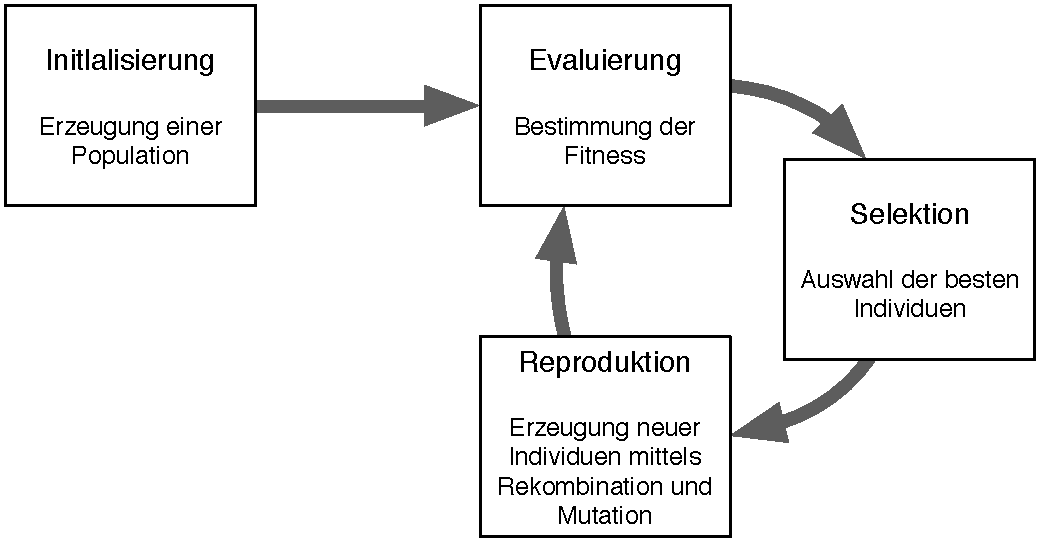
\includegraphics[width=0.8\textwidth]{evo_basic}
\caption{Ablauf evolutionärer Algorithmen}
\label{fig:evo_basic}
\end{figure}

Die einzelnen Komponenten eines evolutionären Algorithmus werden im Folgenden beschrieben. Die Definitionen folgen im Wesentlichen denen von \textcite{tw2008}.

\paragraph{Initialisierung}

Die Population \(P\) stellt eine Menge von Lösungskandidaten dar. Ein Lösungskandidat \(i\) wird als \emph{Individuum} bezeichnet und durch seinen \emph{Genotyp} repräsentiert. Der Genotyp ist die kodierte Repräsentation aller Variablen, die den Lösungskandidaten spezifizieren. Die Variablen werden \emph{Gene} genannt. Während der Initialisierung werden Lösungskandidaten erzeugt, die die Startpopulation des evolutionären Algorithmus bilden. Die Gene jedes Individuums werden üblicherweise zufällig gewählt.

\paragraph{Evaluierung}

Der Evaluierungsschritt dient zur Bestimmung der \emph{Fitness} der Individuen, die noch in der Population enthalten sind. Die Fitness stellt einen Wert dar, der die Güte der durch das Individuum repräsentierten Lösung bezüglich der Problemstellung beschreibt. Die Fitness kann, je nach Optimierungsproblem, entweder absolut oder bezüglich der anderen Individuen der Population bestimmt werden. Somit lässt sich die Funktion zur Bestimmung der Fitness auf die Form \(fitness(i, P)\) generalisieren.

\paragraph{Selektion}

Im Selektionsschritt werden die fittesten Individuen der Population ausgewählt. Alle nicht ausgewählten Lösungskandidaten werden verworfen. Die Selektion kann als Funktion der Form \(select(P, f, s)\) dargestellt werden, wobei \(s\) eine festgelegte Anzahl von Individuen darstellt, die ausgewählt werden sollen.

\paragraph{Reproduktion}

Die Reproduktion dient dazu, aus den im Selektionsschritt ausgewählten Individuen neue Lösungskandidaten zu erzeugen. Dabei werden üblicherweise die Operationen \emph{Rekombination} und \emph{Mutation} verwendet. Bei der Rekombination wird, analog zur Biologie, aus zwei Elternindividuen ein neues Kindindividuum erzeugt. Sie lässt sich als Funktion der Form \(i_n = recombine(i_a, i_b)\) darstellen, wobei \(i_n\) das neue Individuum und \(i_a\) und \(i_b\) die Elternindividuen darstellen. Eine Mutation erzeugt ein neues Individuen durch die Modifikation eines anderen und ist daher durch die Funktion \(i_n = mutate(i_a)\) spezifiziert.

In der Literatur \cite{kw2007, tw2008, dj2006} finden sich für Selektion, Mutation und Rekombination Standardverfahren, die in Hinblick auf das zu lösende Optimierungsproblem ausgewählt werden können. Die konkret implementierten Verfahren werden in \cref{evo_implementation} beschrieben.

Nachdem evolutionäre Algorithmen grundlegend beschrieben wurden, wird im nächsten Abschnitt erläutert, wie die Prioisierung mittels dieser Algorithmenklasse implementiert werden kann.

\subsection{Anwendung zur Prioisierung}

Mit Hilfe von evolutionären Algorithmen kann der Prozess der Prioisierung aus \cref{prioritization} genauer beschrieben werden. \cref{fig:prioritization_evo} zeigt den Prozess mit den Komponenten evolutionärer Algorithmen.

\begin{figure}[h]
\centering
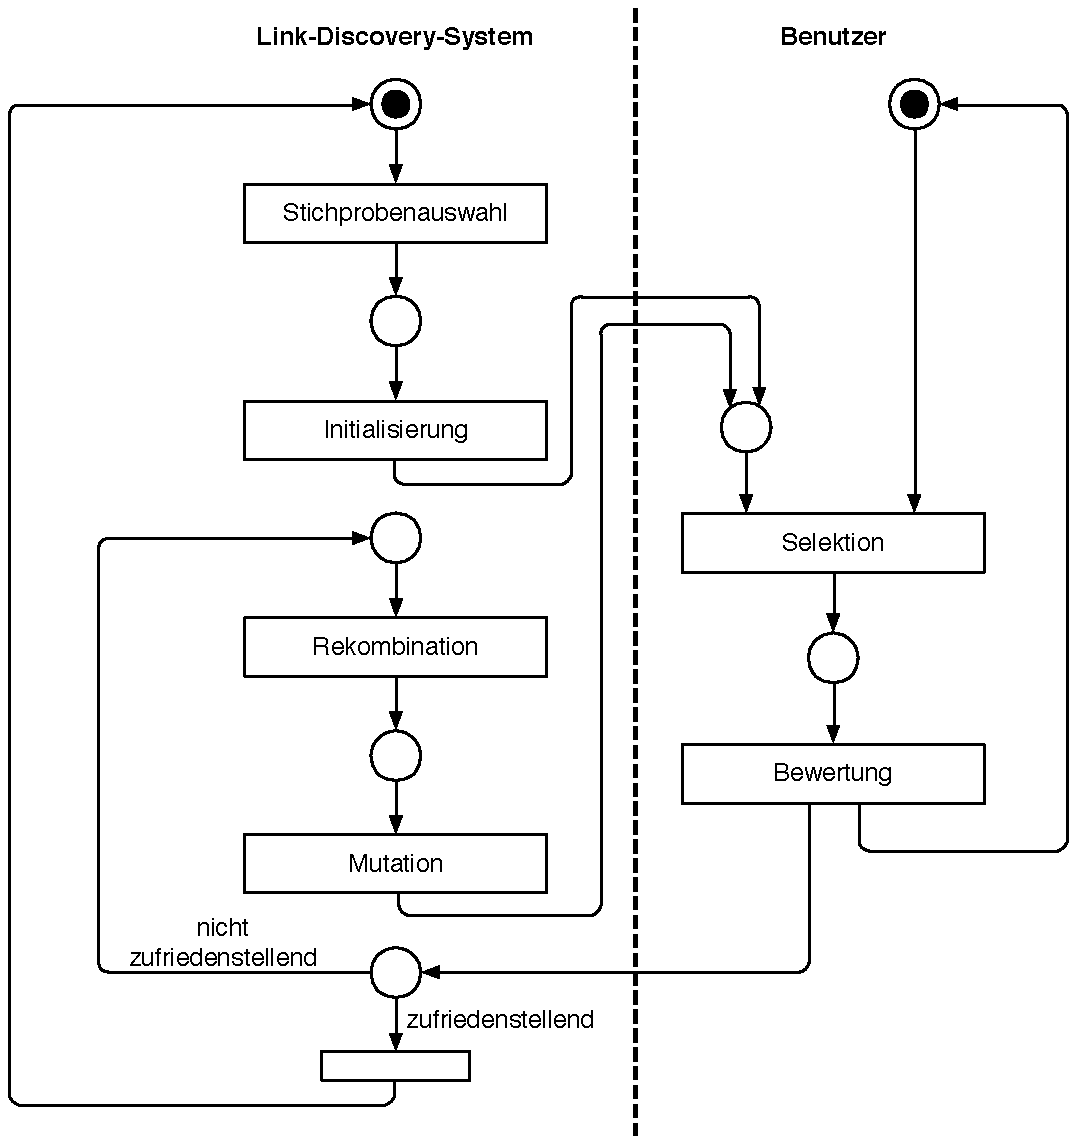
\includegraphics[width=0.8\textwidth]{prioritization_evo}
\caption{FMC--Petri--Netz der Prioisierung mittels evolutionärer Algorithmen}
\label{fig:prioritization_evo}
\end{figure}

Im Gegensatz zu \cref{fig:prioritization} ist zu erkennen, dass die Schritte zur Prioisierungserzeugung mit den Komponenten evolutionärer Algorithmen Initialisierung, Rekombination und Mutation ausgetauscht wurden. Die Selektion wird vom Benutzer vorgenommen, welcher anschließend bewertet, ob die ausgewählten Lösungskandidaten eine zufriedenstellende Prioisierung der Beziehungstypen darstellen.

Nach der Stichprobenauswahl wird für die Stichprobe eine Population von Lösungskandidaten erzeugt. Der Genotyp eines Individuums sollte pro Zusammenhangstyp ein Gewicht enthalten. Jedes Individuum stellt somit eine Gewichtung der Zusammenhangstypen dar.

Da der Algorithmus den Eingriff eines Benutzers erfordert, handelt es sich um einen \emph{interaktiven evolutionären Algorithmus} \cite{ht2001}. Die interaktive Komponente ist hierbei die Selektion, wodurch der Schritt der Evaluierung übersprungen werden kann. Wird die Selektion direkt vom Benutzer ausgeführt, erübrigt sich die Bestimmung eines Fitnesswertes.

Die Schritte der Rekombination und Mutation dienen zur Erzeugung neuer Lösungskandidaten auf Basis der vom Benutzer selektierten Prioisierungen. Sie sollten so gewählt werden, dass genügend unterschiedliche Prioisierungen erzeugt werden, aber dennoch eine Verbesserung über die Generationen erkennbar ist.

Zusammenfassend stellen evolutionäre Algorithmen eine geeignete Methode dar, um die Prioisierung durchzuführen, da die Schritte der Prioisierungserzeugung darauf abgebildet werden können. Die Stichprobenauswahl, die konkret implementierten Komponenten, die Durchführung der Selektion und die Ergebnisse werden in \cref{evo_implementation} detailliert erläutert.

\section{Zusammenfassung}

In diesem Kapitel wurde das Framework zur Link Discovery erläutert. Dies beinhaltet den modellierten Weltausschnitt und dessen Umsetzung auf eine Graph--Datenstruktur. Der Prozess der Erzeugung, Anreicherung und Prioisierung der Beziehungen dieses Modelles wurde definiert und beschrieben. Kookkurrenz wurde als Mittel zur Beziehungserzeugung vorgestellt, die gängigen Maße genannt und die Berechnung erläutert. Ferner wurden mögliche Datenquellen für die Anreicherung diskutiert sowie der Einsatz evolutionärer Algorithmen zur Beziehungsprioisierung beschrieben. Nachdem in diesem Kapitel das Link--Discovery--Framework umfassend behandelt wurde, beschreibt das nächste Kapitel die konkrete Durchführung der Link Discovery.
\chapter{Link--Discovery--Durchführung}
\label{link_discovery}

Dieses Kapitel beschäftigt sich mit den konkret durchgeführten Schritten zur Link Discovery an Beispieldaten. Das Vorgehen und die verwendete Modellierung des Weltausschnittes wurde umfassend in \cref{ld_framework} beschrieben. Im Folgenden wird die initiale Erstellung des Weltausschnittes aus den Daten des Tagging--Systems von Spreadshirt, die Anreicherung durch Clicktracking--Daten, Zerlegung von Wortgruppen in Einzelwörter und Integration des Wortschatzes der Universität Leipzig beschrieben. Anschließend wird die konkrete Priorisierung der Beziehungen mittels evolutionärer Algorithmen erläutert und die Ergebnisse der Link Discovery zusammenfassend ausgewertet.

\section{Initiale Erstellung des Weltausschnittes aus Tagging--Daten}
\label{ld_tags}

Die initiale Erstellung des Weltausschnittes stellt den ersten Schritt des in \cref{ld_process} definierten Link--Discovery--Prozesses dar. Die konkrete Datenquelle, die im Rahmen dieser Arbeit für diesen Schritt verwendet wurde, ist das Tagging--System des Unternehmens Spreadshirt, welches in \cref{tag_sprd} beschrieben wurde. Aus diesen Daten wird mittels Kookkurrenz (siehe \cref{co-occurence}) ein Graph erstellt, der der in \cref{world_graph} erläuterten Repräsentation des Weltausschnittes entspricht. Dieser stellt die Grundlage für alle folgenden Anreicherungsschritte dar. Um diesen initialen Graphen zu berechnen, sind die in \cref{integration_generic} aufgeführten Schritte des Imports, der Bereinigung, der Reduktion, der Transformation und der Integration nötig. Die Umsetzung dieser Schritte wird im folgenden Abschnitt beschrieben.

\subsection{Import}

Die Daten liegen im Quellsystem, einer MySQL--Datenbank, in relationaler Form vor. Somit existieren, dem Datenmodell von Tagging--Systemen in \cref{tagging_data} folgend, Tabellen für Benutzer, Tags, Dokumente und Taggings. Da der Inhalt der Dokumente sowie die Benutzer für die Kookkurrenzberechnung nicht relevant sind, genügt der Import der Tabellen \emph{Tags} und \emph{Taggings}. Das Datenmodell der für den Import benötigten Daten ist in \cref{fig:tag_source_erd} dargestellt.

\begin{figure}[h]
\centering
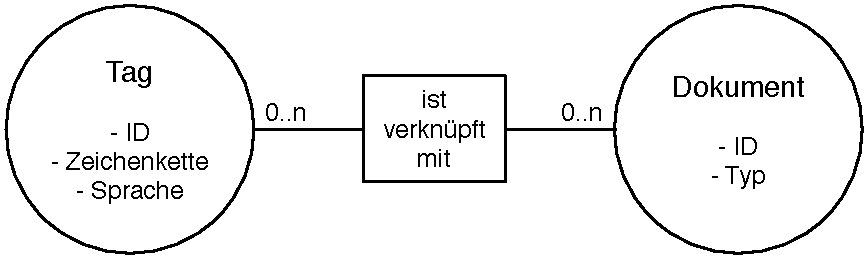
\includegraphics[width=0.6\textwidth]{tag_source_erd}
\caption{FMC--Entity--Relationship--Diagramm der Tagging--Quelldaten}
\label{fig:tag_source_erd}
\end{figure}

Die Tags besitzen, neben einem eindeutigen Bezeichner, die Attribute \emph{tag} für die Zeichenkette und \emph{lang} für die Sprache des Tags. \cref{lst:tag_import_tag} zeigt beispielhaft eine solche Tag--Entität.

\begin{lstlisting}[language=json, label={lst:tag_import_tag}, caption={JSON--Beispiel für einen importierten Tag}, float=h]
{
    "tag_id": 12345,
    "tag": "segeln",
    "lang": "de"
}
\end{lstlisting}

Ein Tagging ist über den eindeutigen Bezeichner des Tags und den eindeutigen Bezeichner des getaggten Dokumentes definiert. Der Schlüssel des Dokumentes setzt sich dabei aus den Attributen \emph{object\_type\_id} und \emph{object\_id} zusammen, da die Dokumente der Spreadshirt--Plattform verschiedene Typen wie  ``Artikel'' oder ``Design'' besitzen können. In \cref{lst:tag_import_link} ist ein Tagging beispielhaft dargestellt.

\begin{lstlisting}[language=json, label={lst:tag_import_link}, caption={JSON--Beispiel für ein importiertes Tagging}, float=ht]
{
    "object_id": 45678
    "object_type_id": 3,
    "tag_id": 12345
}
\end{lstlisting}

Gemäß des Mengengerüstes aus \cref{tag_amount} stehen nach dem Import \num{2072079} Tags und \num{71938905} Taggings für die folgenden Integrationsschritte zur Verfügung.

\subsection{Bereinigung}

An den Tagging--Daten liegen die in \cref{quality} genannten Defekte in Hinblick auf die Datenqualität vor. Diese sollten in einem Bereinigungsschritt reduziert werden. Hierbei liegt das Hauptaugenmerk auf der Erkennung von Duplikaten und später nicht verwertbaren Zeichenketten. Alle durchgeführten Maßnahmen zur Bereinigung beziehen sich hierbei auf das Attribut \emph{tag} eines Tag--Objektes, also der Zeichenkette selbst.

In den unbereinigten importierten Daten existieren keine Duplikate in der Art, dass eine Paarung aus Zeichenkette und Sprache immer nur genau einmal in den Daten vorhanden ist. Jedoch enthalten viele der Tags nicht weiter verwertbare Zeichen wie nicht druckbare ASCII Zeichen, Anführungszeichen, Satzzeichen, Sonderzeichen sowie überflüssige Leerzeichen am Anfang und Ende der Zeichenkette. Außerdem existiert in den importierten Daten eine Unterscheidung zwischen Groß- und Kleinschreibung. Diese Unterscheidung bringt im Kontext der Link Discovery keine Vorteile und kann somit entfernt werden.

\begin{table}[h]
\centering
% \arraystretch}{1.3}
\begin{tabular}{lcl}
    \toprule
    Rohdaten & \phantom{abc} & Bereinigte Daten \\
    \midrule
    \textbackslash u0003\textbackslash r\textbackslash nregenbogen && regenbogen \\
    RegenBogen && regenbogen \\
    "Regenbogen" && regenbogen \\
    regenbogen +einhorn && regenbogen einhorn\\
    \phantom{abc} regenbogen && regenbogen \\
    regenbogen && regenbogen \\
    \bottomrule
\end{tabular}
\caption{Beispiele für die Tag--Bereinigung}
\label{tab:tag_cleaning}
\end{table}

Somit besteht der Bereinigungsschritt darin, nicht verwertbare Zeichen zu entfernen und alle Großbuchstaben in Kleinbuchstaben umzuwandeln. Dadurch entstehen Duplikate, welche im darauf folgenden Reduktionsschritt zusammengeführt werden können. In \cref{tab:tag_cleaning} sind einige Beispiele für die Bereinigungen aufgeführt. Dabei ist gut zu erkennen, dass durch die Bereinigungen Duplikate erzeugt werden.

\subsection{Reduktion}
\label{tag_reduction}

Der Reduktionsschritt dient zur Einschränkung der Gesamtdaten auf eine nützliche oder handhabbare Menge. Außerdem kann durch Reduktion auch die Datenqualität verbessert werden.

Im Fall der Tagging--Daten liegt das Hauptaugenmerk im Reduktionsschritt auf der Entfernung von Duplikaten, die bei der Bereinigung entstanden sind. Gleichzeitig muss sicher gestellt werden, dass keine Informationen über die Verwendung der Tags verloren gehen. Somit besteht die Duplikatentfernung der Tags im Zusammenführen von Datensätzen mit gleichen Zeichenketten und Sprachen. Gleichzeitig werden auch die Taggings zusammengeführt.

\begin{figure}[h]
\centering
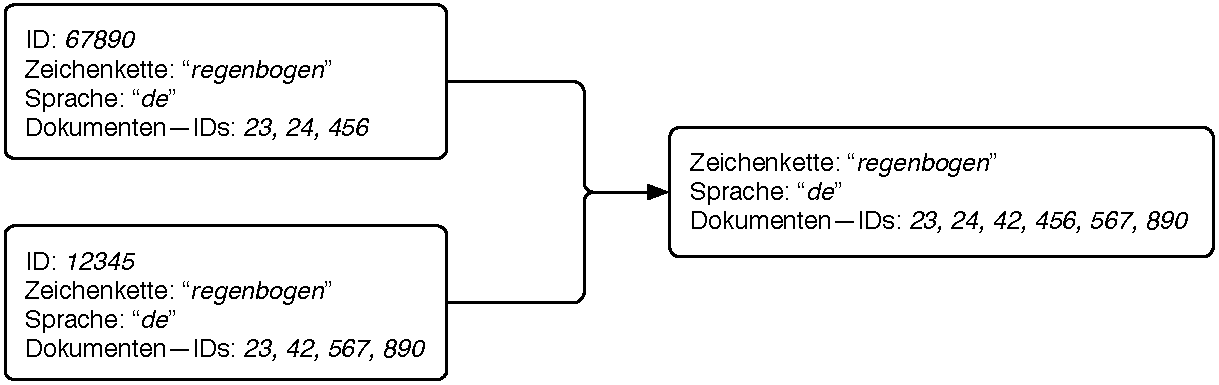
\includegraphics[width=0.9\textwidth]{tag_reduction}
\caption{Beispiel für das Zusammenführen der bereinigten Tags}
\label{fig:tag_reduction}
\end{figure}

Werden die Verknüpfungen zweier Tags mit Dokumenten zusammengeführt, können auch dabei wieder Duplikate entstehen. Diese müssen in diesem Fall entfernt werden, da ein Tag nicht mehrmals mit einem Dokument verknüpft werden kann. Das Zusammenführen von Tags ist exemplarisch in \cref{fig:tag_reduction} dargestellt.

Dabei findet ebenfalls eine Denormalisierung der Daten statt, da alle Dokumente, für die ein Tag vergeben werden, direkt mit in das Tag--Objekt gespeichert werden. Dies ist beispielhaft in \cref{lst:tag_denormalization} abgebildet. Das Attribut \emph{links} enthält alle Verknüpfungen des Tags mit Dokumenten.

\begin{lstlisting}[language=json, label={lst:tag_denormalization}, caption={JSON--Beispiel für die denormalisierten Tagging-Daten}, float=t]
{
    "string": "segeln"
    "language": "de",
    "links": [
        {
            "object_id": 45678, 
            "object_type_id": 3
        },
        {
            "object_id": 98764, 
            "object_type_id": 4
        },
        ...
    ]
}
\end{lstlisting}

Eine weitere im Rahmen dieser Arbeit unternommene Maßnahme zur Datenreduktion bestand darin, sich auf die Menge der Tags zu beschränken, deren Attribut \(lang\) den Wert \emph{de} besitzt. Praktisch handelt es sich um alle Tags, die als deutsch gekennzeichnet in der Datenbank gespeichert sind. Diese Einschränkung wurde vorgenommen, um die zu verarbeitende Datenmenge überschaubar zu halten. Außerdem wird dadurch der nationale Kontext, in dem die Begriffe verwendet wurden, weitestgehend beibehalten.

Ein letzter Reduktionsschritt besteht in der Entfernung der Tags, deren Zeichenketten eine Länge von \num{1} besitzen, da in der deutschen Sprache keine einbuchstabigen Wörter existieren.

Nach der beschriebenen Reduktion befinden sich noch \num{314351} Tags und \num{23255714} Taggings in der Datenbank. Dies entspricht einer Reduktion von ca. \num{68} Prozent gegenüber der importierten Menge von Objekten.

\subsection{Transformation}

Der Transformationsschritt stellt die Überführung der Daten in die in \cref{world_graph} beschriebene Repräsentation des Weltausschnittes dar. Für die Tagging--Daten bedeutet dies eine Umformung in eine Graphenform, wobei die Kanten des Graphen über Kookkurrenz ermittelt werden. Die genaue Umsetzung dieser Transformation mittels des MapReduce--Programmiermodelles wird in \cref{mapreduce_cooccurence} detailliert beschrieben.

Je Tag wird ein während der Transformation ein Knotenobjekt erzeugt. Dieses besitzt als benötigte Attribute die \emph{Zeichenkette} und die \emph{Sprache} des Tags, aus dem es erzeugt wurde und repräsentiert somit einen Begriff des Weltausschnittes. Außerdem wird ein Kontext dieses Begriffes im Rahmen des Tagging--Systems erzeugt. Dieser enthält die Anzahl der Verwendungen des Begriffes als Tag und die eindeutigen Bezeichner der Dokumente, also der Artikel und Designs, die mit dem Begriff getaggt wurden. Weiterhin wird für jedes Knotenobjekt ein global eindeutiger Bezeichner generiert, um die spätere Referenzierung der Knoten zu ermöglichen. \cref{lst:tag_transform_node} zeigt ein Beispiel für ein so erzeugtes Knotenobjekt.

\begin{lstlisting}[language=json, label={lst:tag_transform_node}, caption={JSON--Beispiel für einen aus den Tagging--Daten erzeugten Knoten}, float=h]
{
    "_id" : ObjectId("51efc20147cae77dfc02e0ac"),
    "language" : "de",
    "string" : "mama",
    "tagProperties" : {
        "occurenceCount" : 3,
        "articleCount" : 2,
        "designCount" : 1,
        "articleIDs" : [
            24231101,
            24231105
        ],
        "designIDs" : [
            15514592
        ]
    }
}
\end{lstlisting}

Die Erzeugung der Kanten erfolgt wie in \cref{mapreduce_cooccurence} beschrieben. Für jedes gemeinsame Auftreten von zwei Tags werden zwei Kantenobjekte erzeugt. Diese beschreiben gerichtete Kanten zwischen den Begriffen, die ein gemeinsames Auftreten der Tags repräsentieren. Neben den eindeutigen Bezeichnern der Quell- und Zielknoten enthält das Kantenobjekt den Kantentyp \emph{Tagging--Kookkurrenz} sowie die absolute Anzahl gemeinsamer Vorkommen der Tags und die in \cref{measures} beschriebenen Kookkurrenzmaße. Außerdem erhält die Kante selbst einen global eindeutigen Bezeichner zur Referenzierung. Ein Beispiel für eine aus den Tagging--Daten erzeugte Kante ist in \cref{lst:tag_transform_edge} dargestellt.

\begin{lstlisting}[language=json, label={lst:tag_transform_edge}, caption={JSON--Beispiel für eine aus den Tagging--Daten erzeugte Kante}, float]
{
    "_id" : ObjectId("51efd6f61177ff360605bd99"),
    "source" : ObjectId("51efc1af47cae77dfc00c3f8"),
    "target" : ObjectId("51efc1e047cae77dfc02087c"),
    "type" : "tag-co-occurence",
    "occurences" : 1,
    "dice" : 0.0001317089232795522,
    "jaccard" : 0.00006585879873551106,
    "cosine" : 0.008115343414514944
}
\end{lstlisting}

\subsection{Integration}

Da es sich bei der Integration der Tagging--Daten um die initiale Erstellung des Weltausschnittes handelt, ist der letzte Schritt trivial. Die transformierten Daten müssen lediglich in die Zieldatenbank kopiert werden, da noch keine weiteren Daten vorhanden sind, mit denen sie integriert werden müssen.

\subsection{Ergebnisse}
\label{tagging_results}

Durch die Schritte, die zur Link Discovery aus den Tagging--Daten verwendet wurden, wurden insgesamt \num{314351} Knoten und \num{21834868} Kanten erzeugt.

Eine mögliche Metrik für die quantitativen Eigenschaften der Ergebnisse ist die Verteilung der ausgehenden Kanten, die jeder Knoten besitzt. Diese ist als Histogramm in \cref{fig:hist_only_tags} dargestellt. Hierbei ist anzumerken, dass die Klassen des Histogrammes exponentiell breiter werden, um Knoten, die sehr viele Kanten besitzen, im Histogramm darstellen zu können.

\begin{figure}[ht]
\centering
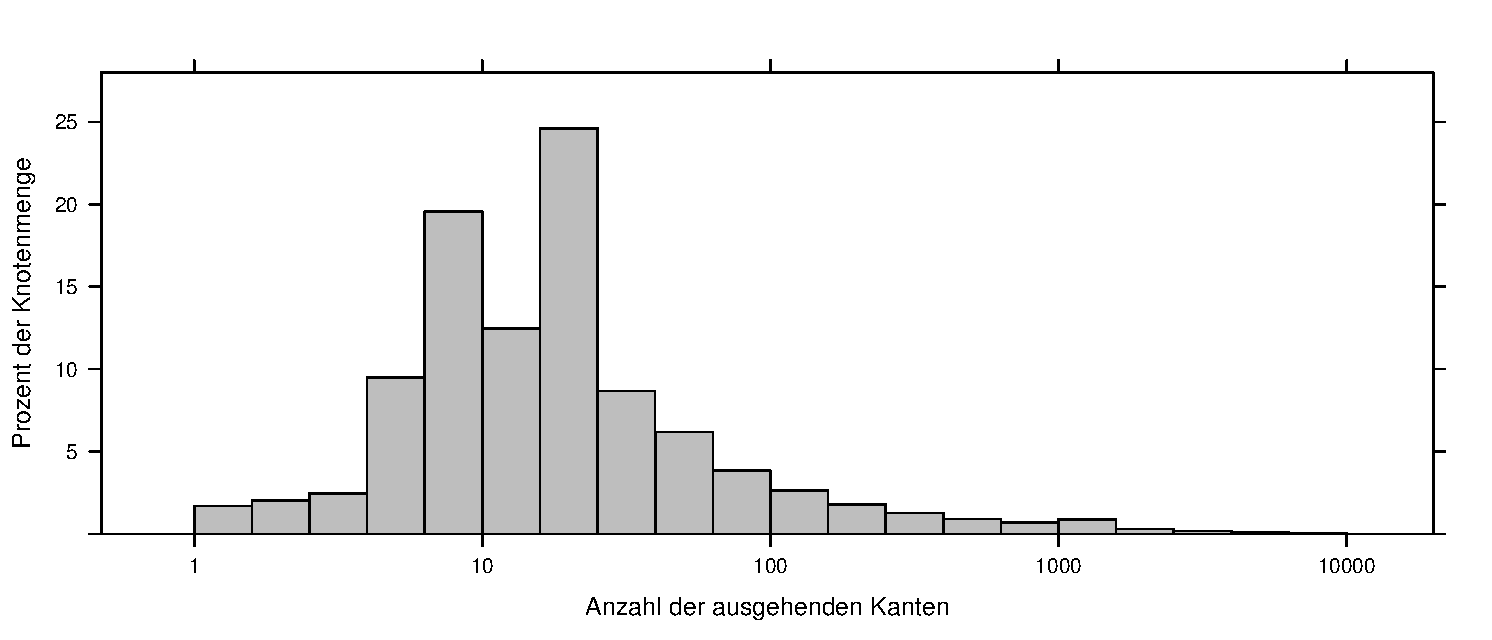
\includegraphics[width=\textwidth]{hist_only_tags}
\caption{Histogramm der Verteilung der Tagging--Kookkurrenz--Kanten}
\label{fig:hist_only_tags}
\end{figure}

\cref{tab:only_tags} zeigt die statistischen Kennzahlen Minimum, erstes Quartil, Median, drittes Quartil, Maximum und Durchschnitt der Verteilung der Kanten nach Berechnung der Tagging--Kookkurrenz.

\begin{table}[ht]
\centering
\begin{tabular}{lr}
    \toprule
    Kennzahl & Wert \\
    \midrule
    \(min\) & \num{0} \\
    \(Q_{0.25}\) & \num{9} \\
    \(Q_{0.5}\) & \num{16} \\
    \(Q_{0.75}\) & \num{29} \\
    \(max\) &  \num{35169} \\
    \(avg\) &  \num{74,64} \\
    \bottomrule
\end{tabular}
\caption{Statistische Kennzahlen für die Verteilung der Tagging--Kookkurrenz--Kanten}
\label{tab:only_tags}
\end{table}

Bei der Interpretation dieser Daten fällt auf, dass die Anzahl der ausgehenden Kanten sehr ungleich verteilt ist. Es existieren sehr viele Knoten mit wenigen Kanten und sehr wenige Knoten mit vielen Kanten. Der verhältnismäßig hohe Median sagt allerdings ebenfalls aus, dass die Hälfte aller Knoten mehr als \num{16} ausgehende Kanten besitzen. Dies lässt jedoch keine Aussage über die inhaltliche Qualität der erzeugten Zusammenhänge zu. Diese kann nur auf Basis eines einzelnen Begriffes und dessen Beziehungen beurteilt werden.

Der Begriff, der das Maximum von \num{35169} ausgehenden Kanten erreicht, ist der Begriff ``liebe''. Dieser Begriff zählt zu den meistgesuchten und verwendeten Tags auf der Spreadshirt--Plattform. Dies spiegelt sich offensichtlich auch darin wieder, dass er zusammen mit \num{35169} anderen unterschiedlichen Tags vergeben wurde.

Nachdem in diesem Abschnitt die Integration der Tagging--Daten beschrieben wurde, beschäftigt sich der folgende Abschnitt mit der Anreicherung des Weltausschnittes mit den Daten des Clicktracking--Systems von Spreadshirt.

\section{Anreicherung des Weltausschnittes mit Clicktracking--Daten}
\label{clicktracking}

Spreadshirt betreibt ein Clicktracking--System (siehe \cref{clicktracking_theo}), welches die Klicks der Benutzer auf Artikel und Designs auf Suchergebnisseiten aufzeichnet. Dabei ist unerheblich, ob der Benutzer bei Spreadshirt registriert und angemeldet ist. Dieses System sammelt Daten von beiden Spreadshirt--Plattformen (siehe \cref{platforms}). In \cref{fig:search_result} ist beispielhaft eine Suchergebnisseite der Spreadshirt--Plattform abgebildet, welche die gefundenen Designs für eine Suchanfrage auflistet.

\begin{figure}[t]
\centering
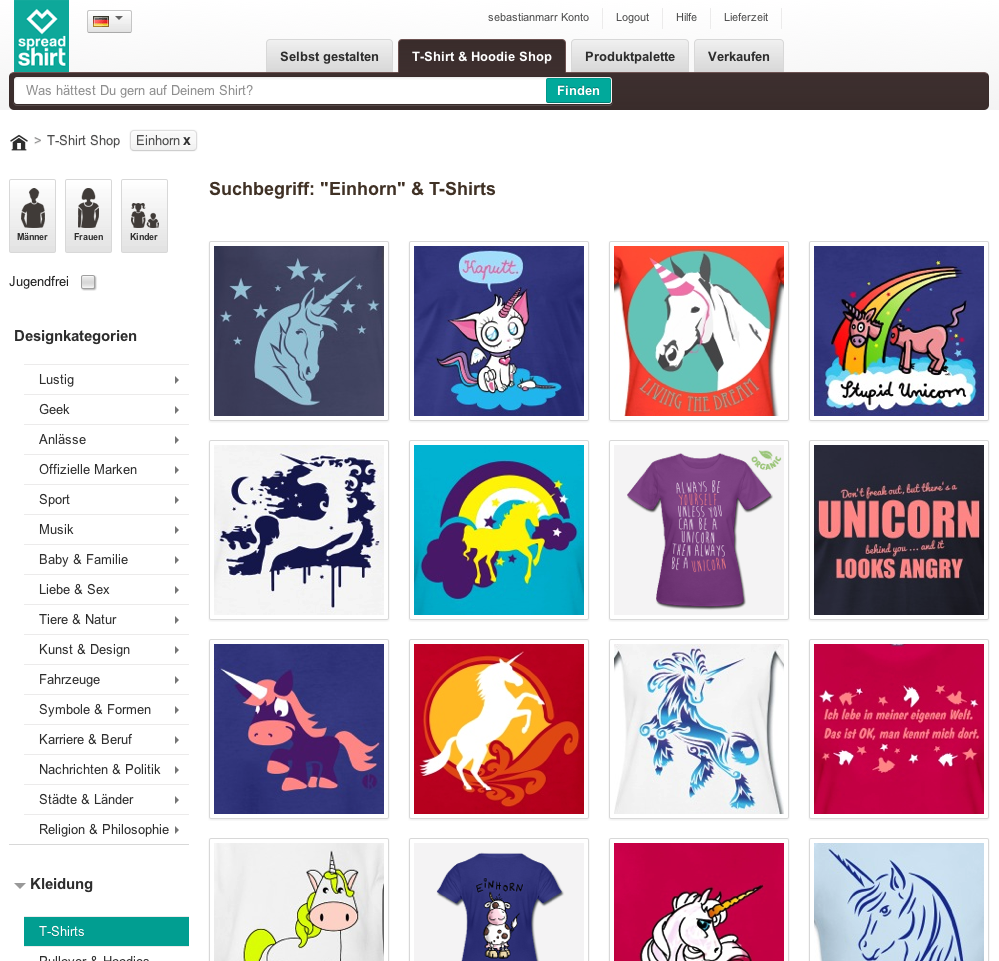
\includegraphics[scale=0.25]{search_result}
\caption{Beispiel für eine Spreadshirt--Suchergebnisseite}
\label{fig:search_result}
\end{figure}

Die von diesem System erzeugten Daten können für die Link Discovery von großer Bedeutung sein, da sie eine andere Perspektive auf die Begriffe im Graphen liefern. Die Tags liefern die Sicht der Partner, also der Personen, die Inhalte hochladen und verkaufen möchten. Die Klicks beschreiben die Sicht der Käufer, also der Personen, die nach Inhalten suchen. Durch die Auswertung der Clicktracking--Daten ergibt sich also die Möglichkeit, eine Form der Validierung der durch Partner vergebenen Metadaten zu erhalten. Die Annahme hierbei ist, dass Käufer nur auf Suchergebnisse klicken, die eine inhaltliche Relevanz zum eingegebenen Suchbegriff besitzen und somit ihren Erwartungen bezüglich des Suchbegriffes gerecht werden.

Wie bereits für die Tagging--Daten, werden im Folgenden auch für das Clicktracking die Schritte Import, Bereinigung, Reduktion, Transformation und Integration (siehe \cref{integration_generic}) näher erläutert. Der Ansatz zur Erzeugung der Verbindungen ist, wie schon bei den Tagging--Daten, kookkurrenzbasiert.

\subsection{Import}
\label{click_import}

Das Clicktracking--System erzeugt Dateien im JSON--Format, die zu jedem Klick auf einer Ergebnisseite die wesentlichen Informationen enthalten. Pro Klick ist ein JSON--Dokument in den Dateien abgespeichert. Ein Beispiel für ein solches Dokument ist in \cref{lst:click_raw} dargestellt.

\begin{lstlisting}[language=json, label={lst:click_raw}, caption={JSON--Beispiel für ein Clicktracking--Rohdokument}, float]
{
    "date": "01.07.2013 00:09:31_633",
    "path": "/track/eu/205909/1E3B6E3E-4496-C51A14A8FA25/2.10.4/list",
    "params": {
        "locale": "[de_DE]",
        "search-query": "[biene]",
        "cl": "[a18869874, p25446183, i49]"
    }
}
\end{lstlisting}

Ein Clicktracking--Dokument enthält die Attribute \emph{Datum}, \emph{Pfad}, \emph{Gebietsschema}, \emph{Suchbegriff} und die Daten des eigentlichen Klicks, also den geklickten \emph{Artikel}, das geklickte \emph{Produkt} und den \emph{Index}, also die Position des geklickten Inhaltes auf der Suchergebnisseite. Die Unterscheidung zwischen Produkt und Artikel ist im Domänenmodell von Spreadshirt begründet (siehe auch \cref{spreadshirt}) und für die Link Discovery nicht von Interesse. Es genügt, den geklickten Artikel im Weiteren näher zu betrachten.

Auffällig ist, dass die Möglichkeiten des JSON--Formates bei der Speicherung der Klickdaten nicht vollständig ausgenutzt wurden. So sind die Werte, die das geklickte Dokument beschreiben, als Zeichenkette abgelegt und zusätzlich die eindeutigen Bezeichner mit einem Buchstaben versehen, der ihren Typ angibt. Des weiteren enthalten  das Gebietsschema und der Suchbegriff zusätzliche eckige Klammern. Diese Defekte sollten im Bereinigungsschritt beseitigt werden, um ein nutzbareres Datenformat zu erhalten.

Da das Clicktracking--System zum Zeitpunkt des Imports erst 3 Monate Daten aufzeichnete, standen \num{2249942} solcher Klickdokumente zur Verfügung.

\subsection{Bereinigung}

Im Bereinigungsschritt sollten zunächst die im vorherigen Abschnitt genannten Defekte an den Daten des Clicktracking--Systems beseitigt werden. Dazu gehört die Entfernung der eckigen Klammern in Suchbegriff und Gebietsschema und die Extraktion des eindeutigen Bezeichners des geklickten Artikels. Aus dem Gebietsschema ist nur die Sprache von Interesse. Außerdem wurden für den Suchbegriff die gleichen Bereinigungsoperationen wie für die Tagging--Daten vorgenommen, also die Entfernung von überflüssigen Leerzeichen, Groß-/Kleinschreibung, nicht druckbarer Sonderzeichen und Satzzeichen.

Im Bereinigungsschritt werden so auch einfacher verarbeitbare Dokumente erzeugt, da die Möglichkeiten des JSON--Formates besser ausgenutzt werden. \cref{lst:tag_cleanup} zeigt das Ergebnis der Bereinigung des in \cref{click_import} gezeigten Beispieldokumentes.

\begin{lstlisting}[language=json, label={lst:tag_cleanup}, caption={JSON--Beispiel für die Bereinigung der Clicktracking--Dokumente}, float]
{
    "_id": ObjectId("51e7b1e0417498f9c6868939"),
    "query" : "biene",
    "date" : "2013-07-01T00:09:31.633Z",
    "articleId" : 18869874,
    "index" : 57,
    "language" : "de"
}
\end{lstlisting}

\subsection{Reduktion}

Die Reduktion der Clicktracking--Daten besteht zum einen aus einer Duplikatentfernung, zum anderen aus der Einschränkung der Sprache.

Im Sinne der Kookkurrenz ist es nicht von Bedeutung, wenn Paare aus Suchbegriffen und geklickten Artikeln mehrfach auftauchen, da hierfür nur das gemeinsame Auftreten unterschiedlicher Suchbegriffe betrachtet wird. Somit besteht die Duplikatentfernung lediglich darin, aus mehrfach vorkommenden Artikel-/Klickpaaren genau eines auszuwählen.

Außerdem erfolgte, wie schon bei den Tag--Daten, eine Einschränkung auf Klicks, die als \emph{deutsch} gekennzeichnet sind.

Nach dem Reduktionsschritt verblieben zur Transformation noch \num{411341} Klicks.

\subsection{Transformation}

Der Transformationsschritt dient zur Umformung der Clicktracking--Daten in die Graphenrepräsentation des Weltausschnittes aus \cref{world_graph}. Diese Umformung wird durch die Ermittlung von Kookkurrenz durchgeführt. Diese bestimmt sich hierbei daraus, welche Suchbegriffe zum Klick auf einen Artikel geführt haben. Wird ein Artikel zu mehreren Suchbegriffen geklickt, liegt die Vermutung nah, dass zwischen den Suchbegriffen ein irgendwie gearteter Zusammenhang besteht.

Ziel der Transformation ist somit die Erzeugung von Knoten und Kanten. Die Knoten werden zusätzlich mit einem Kontext verknüpft, der die Eigenschaften des durch den Knoten repräsentierten Begriffes im Kontext des Clicktracking--Systems. Konkret sind dies die Artikel, die zu dem Begriff als Suchbegriff geklickt wurden. \cref{lst:click_node} zeigt einen aus den Clicktracking--Daten erzeugten Knoten.

\begin{lstlisting}[language=json, label={lst:click_node}, caption={JSON--Beispiel für ein aus den Clicktracking--Daten erzeugtes Knotenobjekt}, float]
{
    "_id": ObjectId("51e7f1e04146498f9c6868945"),
    "string": "biene",
    "language": "de",
    "clickProperties": [
        { "articleId": 4512 },
        { "articleId": 4794 },
        ...
    ]
}
\end{lstlisting}

Die Kanten besitzen die gleiche Form wie die Kookkurrenzkanten, die bei der Integration der Tagging--Daten erzeugt wurden. Lediglich der Typ der Kanten ist unterschiedlich und lautet \emph{Clicktracking--Kookkurrenz}. Ein Beispiel für eine solche Kante ist in \cref{lst:click_edge} dargestellt.

\begin{lstlisting}[language=json, label={lst:click_edge}, caption={JSON--Beispiel für ein aus den Clicktracking--Daten erzeugtes Kantenobjekt}]
{
    "_id": ObjectId("51e91aff3b6a20bfd68c468a")
    "source" : ObjectId("51e91af93b6a20bfd68b0bed"),
    "target" : ObjectId("51e91aff3b6a20bfd68c463e"),
    "type": "click-co-occurence",
    "occs" : 1,
    "dice" : 0.003883495145631068,
    "jaccard" : 0.0019455252918287938,
    "cosine" : 0.04410810913912309
}
\end{lstlisting}

Die Durchführung des Transformationsschrittes erfolgte mittels MapReduce (siehe \cref{mapreduce_cooccurence}). Dadurch wurden \num{92727} Knoten und \num{310860} Kanten erzeugt.

\subsection{Integration}
\label{click_integration}

Die Integration der erzeugten Daten stellt eine Vereinigung des vorhandenen Weltausschnittes mit dem im Transformationsschritt erzeugten Graphen dar.

Die Knotenmenge wird derart vereinigt, das sie die Eigenschaft behält, dass Paare aus Sprache und Zeichenkette eindeutig sind. Somit werden bei bereits vorhandenen Knoten die zusätzlichen Informationen bezüglich des Clicktrackings als Attribute hinzugefügt. Existiert eine Kombination aus Sprache und Zeichenkette noch nicht im Zielgraph, so wird der entsprechende Knoten eingefügt.

Da die erzeugten Kanten einen noch nicht im Graph vorhandenen Typ besitzen, müssen keine Kanten zusammengeführt werden. Jedoch werden die Bezeichner der Ziel- und Quellknoten entsprechend angepasst, wenn bei der Integration der Knoten eine Zusammenführung stattgefunden hat.

\subsection{Ergebnisse}

Durch die auf die Clicktracking--Daten angewendeten Link--Discovery--Schritte wurden dem Weltausschnitt \num{78237} neue Begriffe und \num{310860} neue Zusammenhänge vom Type \emph{Clicktracking--Kookkurrenz} hinzugefügt.

Wie schon für die Tagging--Daten in \cref{tagging_results}, wird im folgenden die Verteilung der Clicktracking--Kanten je Knoten als Metrik für die Ergebnisse der Clicktracking--Integration verwendet. Diese ist in \cref{fig:hist_only_clicktracking} als Histogramm mit exponentiell wachsenden Klassen dargestellt.

\begin{figure}[t]
\centering
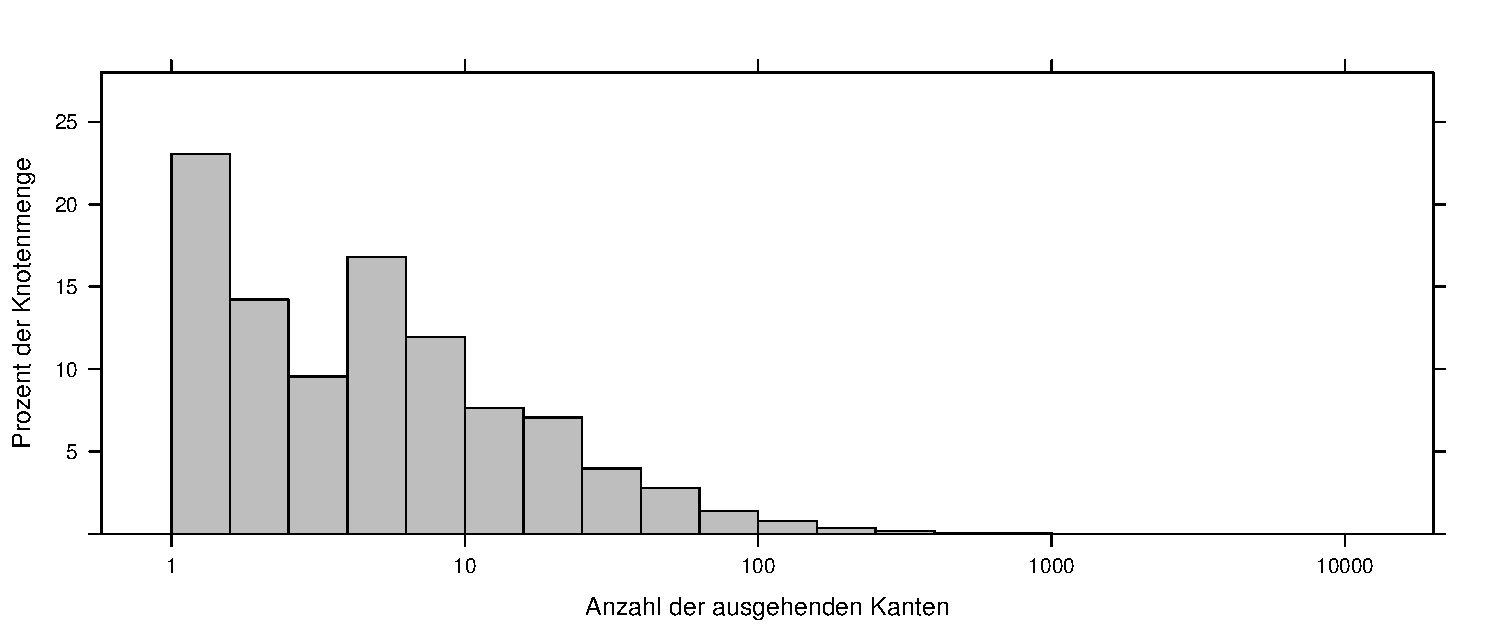
\includegraphics[width=\textwidth]{hist_only_clicktracking}
\caption{Histogramm der Verteilung der Clicktracking--Kookkurrenz--Kanten}
\label{fig:hist_only_clicktracking}
\end{figure}

\cref{tab:only_clicktracking} zeigt die statistischen Kennzahlen Minimum, erstes Quartil, Median, drittes Quartil, Maximum und Durchschnitt der Verteilung der Kanten nach Berechnung der Clicktracking--Kookkurrenz.

Bei der Interpretation dieser Daten fällt auf, dass im Vergleich zu den Tagging--Daten zum einen deutlich weniger Kanten, zum anderen auch durchschnittlich weniger Kanten pro Knoten erzeugt wurden. So muss bei circa einem Viertel der Knoten, die Kanten vom Typ Clicktracking--Kookkurrenz besitzen, mit zwei oder weniger Beziehungen gerechnet werden. Durch die geringe Kantenanzahl wird die Gesamtverteilung der Kanten jedoch nicht wesentlich beeinflusst (siehe \cref{lda_results}).

\begin{table}[h]
\centering
\begin{tabular}{lr}
    \toprule
    Kennzahl & Wert \\
    \midrule
    \(min\) & \num{1} \\
    \(Q_{0.25}\) & \num{2} \\
    \(Q_{0.5}\) & \num{4} \\
    \(Q_{0.75}\) & \num{10} \\
    \(max\) &  \num{1688} \\
    \(avg\) &  \num{12} \\
    \bottomrule
\end{tabular}
\caption{Statistische Kennzahlen für die Verteilung der Clicktracking--Kookkurrenz--Kanten}
\label{tab:only_clicktracking}
\end{table}

Nachdem die Anreicherung der Clicktracking--Daten durchgeführt wurde, beschäftigt sich der folgende Abschnitt mit der Anreicherung durch die Zerlegung von Wortgruppen in Einzelwörter.

\section{Anreicherung des Weltausschnittes durch Zerlegung von Wortgruppen}
\label{decomposition}

Die Zerlegung von Tags, die aus mehr als einem Wort bestehen, ist ein Anreicherungsschritt durch das Mining von schon im Weltausschnitt vorhandenen Daten (siehe \cref{enrichment_mining}). Neben der Erzeugung zusätzlicher Verbindungen ist er für weitere Integrationsschritte von Nutzen, da es Vorteile bringt, wenn möglichst viele Einzelwörter im Weltausschnitt gespeichert sind (siehe \cref{wortschatz}).

\subsection{Vorgehensweise}

Zum Zeitpunkt des Importes befanden sich \num{147364} Begriffe im Weltausschnitt, die aus mehreren Wörtern bestehen. Dies entspricht \num{47} Prozent aller bereinigten deutschen Tags. Dieser Umstand legt die Vermutung nahe, dass in diesen zusammengesetzten Tags auch Wörter enthalten sind, die nicht als Einzelwörter existieren.

\begin{figure}[h]
\centering
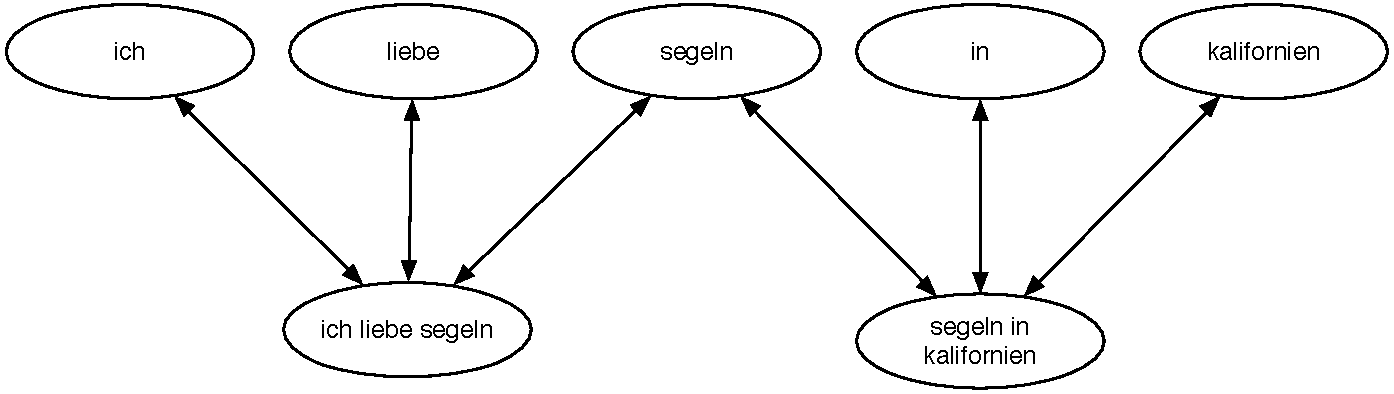
\includegraphics[width=\textwidth]{decomposition}
\caption{Beispielhafter Graphausschnitt nach der Zerlegung}
\label{fig:decomposition}
\end{figure}

Werden diese Begriffe in ihre Einzelwörter zerlegt, entstehen einerseits unter Umständen neue Begriffe, andererseits können in diesem Schritt Zusammenhänge vom Typ \emph{Zerlegung} beziehungsweise \emph{Zusammensetzung} eingefügt werden. Somit sind nach dem Schritt der Zerlegung weitere Informationen über den Kontext, in dem Wörter verwendet werden, verfügbar. \cref{fig:decomposition} zeigt beispielhaft das Ergebnis einer solchen Zerlegung.

\subsection{Ergebnisse}

Durch die Anwendung des Zerlegungsschrittes auf die vorhandenen Begriffe wurden insgesamt \num{38349} neue Knoten und \num{1238900} neue Kanten erzeugt, die für spätere Analyseschritte genutzt werden können.

Die Verteilung der erzeugten Kanten über alle Knoten, die von der Zerlegung betroffen sind, ist in \cref{fig:hist_only_decomposition} als Histogramm dargestellt. Statistische Kennzahlen dieser Verteilung sind in \cref{tab:only_decomposition} aufgeführt.

\begin{figure}[h]
\centering
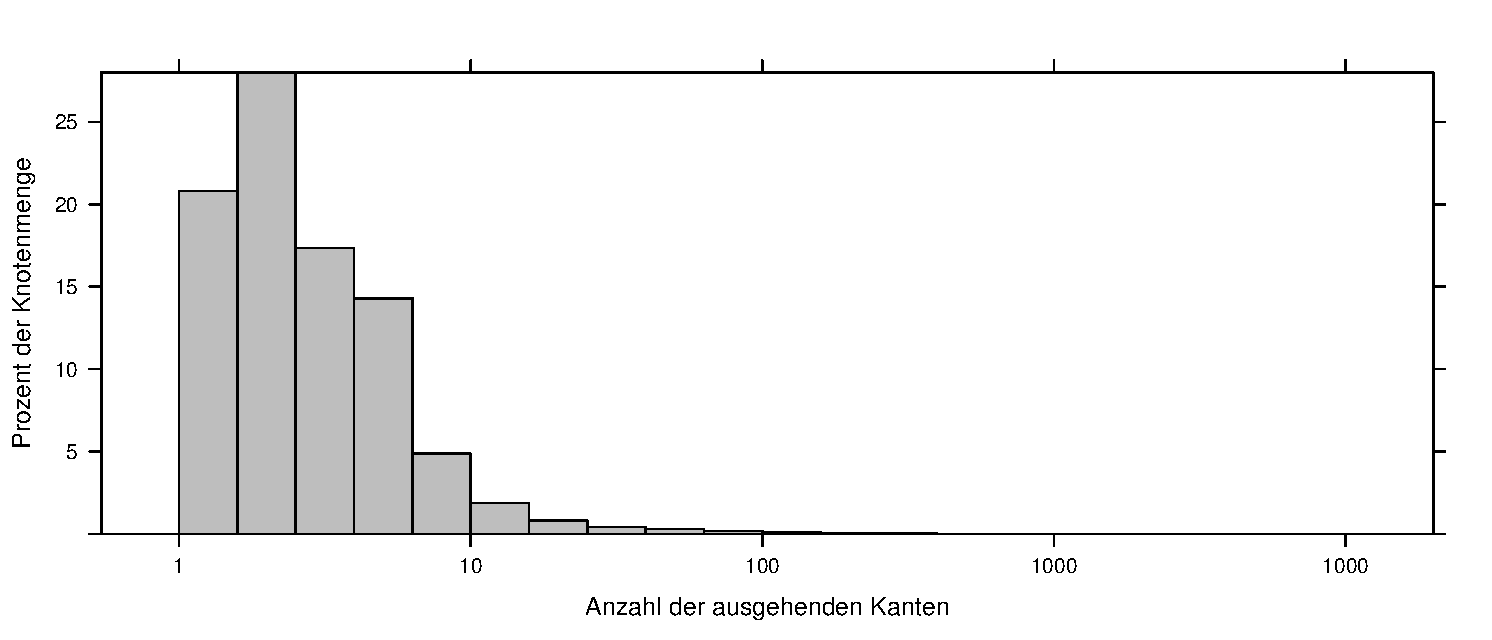
\includegraphics[width=\textwidth]{hist_only_decomposition}
\caption{Histogramm der Verteilung der Zerlegungs-- und Zusammensetzungskanten}
\label{fig:hist_only_decomposition}
\end{figure}

\begin{table}[h]
\centering
\begin{tabular}{lr}
    \toprule
    Kennzahl & Wert \\
    \midrule
    \(min\) & \num{1} \\
    \(Q_{0.25}\) & \num{2} \\
    \(Q_{0.5}\) & \num{2} \\
    \(Q_{0.75}\) & \num{3} \\
    \(max\) &  \num{5215} \\
    \(avg\) &  \num{4,358} \\
    \bottomrule
\end{tabular}
\caption{Statistische Kennzahlen für die Verteilung der Zerlegungs-- und Zusammensetzungskanten}
\label{tab:only_decomposition}
\end{table}

Bei der Zerlegung wurden somit deutlich weniger Kanten pro Knoten erzeugt, als noch bei den Tagging-- und Clicktracking--Daten. Nur ein Viertel der betreffenden Knoten besitzen mehr als drei Kanten vom Typ \emph{Zerlegung} oder \emph{Zusammensetzung}. Der Einfluss der Zerlegung auf den gesamten Datenbestand wird in \cref{lda_results} dargestellt.

Nachdem im Zerlegungsschritt Einzelwörter erzeugt wurden, können diese im folgenden Abschnitt für den Import der Wortschatz--Daten genutzt werden.

\section{Anreicherung des Weltausschnittes mit Wortschatz-Daten}
\label{wortschatz}

Wie in \cref{lexical_sources} bereits einführend beschrieben, betreibt die Universität Leipzig ein Wortschatz--Projekt \cite{ws2013}. Im Rahmen dieses Projektes wird durch die Analyse von großen Textmengen eine Datenbank deutscher Wörter, deren Bedeutungen, grammatikalische Eigenschaften, Häufigkeiten und Kookkurrenzen in Texten und Beziehungen zu anderen Wörtern aufgebaut. Somit stellt dieses Projekt eine sehr gute Möglichkeit dar, weitere Zusammenhänge zwischen den schon im Weltausschnitt vorhandenen Begriffen herzustellen. Neben den Daten, die im Spreadshirt--Kontext entstehen, können somit auch allgemeine lexikalische Daten hinzugefügt und für spätere Analysen genutzt werden.

Neben einem Webportal \cite{ws2013} stellt dieses Projekt eine API bereit, über die die Daten des Wortschatzes programmatisch abgefragt werden können. Diese API wurde mittels einer Bibliothek für die Programmiersprache Ruby \cite{wlapi2013} im Rahmen dieser Arbeit für einen weiteren Integrationsschritt zur Link Discovery genutzt. Dazu wurden die Informationen \emph{Grundform}, \emph{Wortformen}, \emph{Kategorien}, \emph{Synonyme} und \emph{Thesaurus--Beziehungen} ausgewertet (siehe \cref{used_sources}).

Wie bereits für die anderen Datenquellen, werden im Folgenden auch für den Wortschatz die Schritte des Imports, der Bereinigung, der Reduktion, der Transformation und der Integration beschrieben (siehe \cref{integration_generic}).

\subsection{Import}

\begin{lstlisting}[language=json, label={lst:wortschatz_import}, caption={JSON--Beispiel für Rohdaten aus dem Wortschatz}, float]
{
    "_id" : ObjectId("51f7aa06eba16044e900015a"),
    "string" : "Kopf",
    "baseform" : [ 
        "Kopf", 
        "N"
    ],
    "domain" : [ 
        "Medizin", 
        "Anatomie", 
        "Literarische/Motive/Stoffe/Gestalten", 
        "Körperteile"
    ],
    "synonyms" : [  
        "Chef", 
        "Figur", 
        "Gestalt", 
        "Haupt", 
        "Jemand", 
        "Individuum", 
        "Figur"
    ],
    "thesaurus" : [ 
        "Titel", 
        "Hand", 
        "Kopf", 
        "Mensch", 
        "Gesicht", 
        "Spitze", 
        "Arm", 
        "Gestalt"
    ],
    "wordforms" : [ 
        "Kopf", 
        "Köpfe", 
        "Köpfen", 
        "Kopfes", 
        "Kopfs"
    ]
}
\end{lstlisting}

Da für die Anfrage an die Wortschatz--API nur Einzelwörter und keine Wortgruppen genutzt werden können, muss eine Auswahl der anzufragenden Daten getroffen werden. Im Anreicherungsschritt der Zerlegung von Wortgruppen wurden aus allen zu diesem Zeitpunkt vorhandenen Begriffen Einzelwörter gebildet (siehe \cref{decomposition}). Diese können nun beim Import der Wortschatz--Daten genutzt werden, um die Anfragen zu formulieren. Zum Zeitpunkt des Importes standen \num{197614} Einzelwörter zur Verfügung. Da die im Weltausschnitt gespeicherten Daten keine Groß- und Kleinschreibung enthalten, die Wortschatz--API diese jedoch berücksichtigt, wurde jedes Wort jeweils mit großem und kleinem Anfangsbuchstaben angefragt. Somit wurde die doppelte Menge an Rohdaten, \num{395228} Objekte, erzeugt.

\cref{lst:wortschatz_import} zeigt beispielhaft ein importiertes Objekt des Wortschatzes nach dem Import. Dieses enthält Listen von \emph{Grundformen} mit der entsprechenden Wortform als Kürzel, den \emph{Kategorien} des Wortes, \emph{Synonymen}, \emph{Thesaurus-Beziehungen} sowie \emph{Wortformen} als Attribute.

Hierbei ist zu beachten, dass nicht alle Attribute bei allen Wörtern vorhanden sind. Dies hängt davon ab, ob der Wortschatz die Informationen zur Verfügung stellen kann. Somit ist es auch möglich, dass Objekte importiert werden, die keine zusätzlichen Informationen enthalten.

\subsection{Bereinigung}

Zur Bereinigung der importierten Wortschatz--Daten muss in einem ersten Schritt die Groß- und Kleinschreibung entfernt werden, da diese an erster Stelle nur für die Anfragen an die API wieder in den Datenbestand eingeführt wurde.

Weiterhin werden die Kategorien ``Vorname'' und ``Nachname'' entfernt, da diese an über \num{25000} Wörter vergeben sind und somit für die Verwendung zur Link Discovery ungeeignet sind und zu viele irrelevante Kanten erzeugen würden.

\begin{lstlisting}[language=json, label={lst:word_baseform}, caption={JSON--Beispiel für die Umformung der Grundform eines Wortes}, float]
{
    _id: ...,
    string: "Kopfs",
    baseform: {
        word: "Kopf",
        type: "N"
    }
}
\end{lstlisting}

Ein letzter Bereinigungsschritt besteht in der Veränderung des Formates der Grundform des Wortes. Die Wortschatz--API liefert lediglich ein Array, in dem das erste Element die Grundform und das zweite Element die Wortart ist. Zur Bereinigung wird diese Eigenschaft in ein geeignetes JSON--Format überführt, welches in \cref{lst:word_baseform} dargestellt ist.

\subsection{Reduktion}

Der Reduktionsschritt besteht in der Zusammenführung von Objekten, die die gleiche Zeichenkette enthalten. Diese Duplikate sind bei der Entfernung der Groß-- und Kleinschreibung im Bereinigungsschritt entstanden. Wie schon im Reduktionsschritt der Daten des Tagging--Systems (\cref{tag_reduction}), muss auch hierbei das Entstehen neuer Duplikate vermieden werden. Dies bedeutet, dass Listen der Wortbeziehungen ebenfalls zusammengeführt werden, wobei jedes Wort nur einmal enthalten sein darf. Die Reduktion ist beispielhaft in \cref{fig:wortschatz_reduction} dargestellt. Dabei ist zu beachten, dass bei der Zusammenführung mehrere Grundformen entstehen können, wodurch dieses Attribut in ein Array umgewandelt wird.

\begin{figure}
\centering
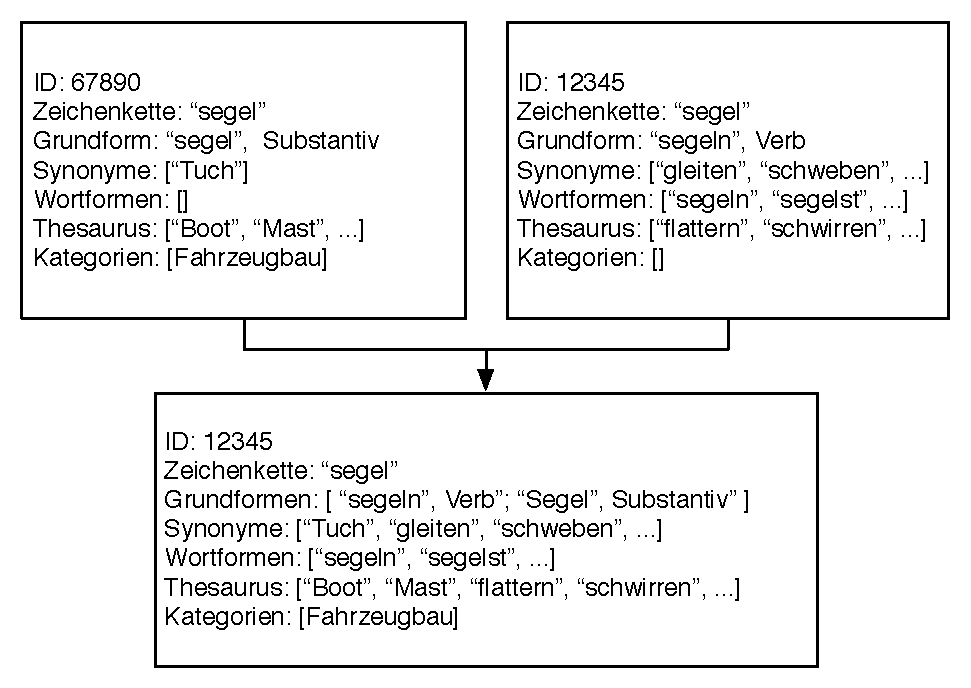
\includegraphics[width=\textwidth]{wortschatz_reduction}
\caption{Reduktion der Wortschatz--Daten}
\label{fig:wortschatz_reduction}
\end{figure}

Durch die Reduktion wird die Anzahl der Dokumente wieder auf die ursprüngliche Menge von Einzelwörtern reduziert und beträgt demnach \num{197614}.

\subsection{Transformation}

Die Transformation der Wortschatz--Daten besteht, wie bereits bei den anderen Datenquellen, in einer Überführung in die Graphenrepräsentation des Weltausschnittes aus \cref{world_graph}. 

Die Knoten repräsentieren alle Wörter, die durch die Benutzung der Wortschatz--API bekannt sind. Dazu zählen einerseits sowohl die angefragten Wörter, als auch die von der API zurückgegebenen Wortbeziehungen. Der Kontext dieser durch die Knoten repräsentierten Begriffe enthält die Rohdaten des Wortschatzes, um sie bei gegebenenfalls stattfindenden späteren Analysen nutzen zu können.

Die Kanten die Attribute \emph{Synonyme}, \emph{Thesaurus}, \emph{Grundform} und \emph{Wortformen} können direkt aus den entsprechenden Attributen erzeugt werden und besitzen die entsprechenden Kantentypen. Sie enthalten keine weiteren Attribute, da über diese Beziehungen keine weiteren Informationen verfügbar sind.

\begin{figure}
\centering
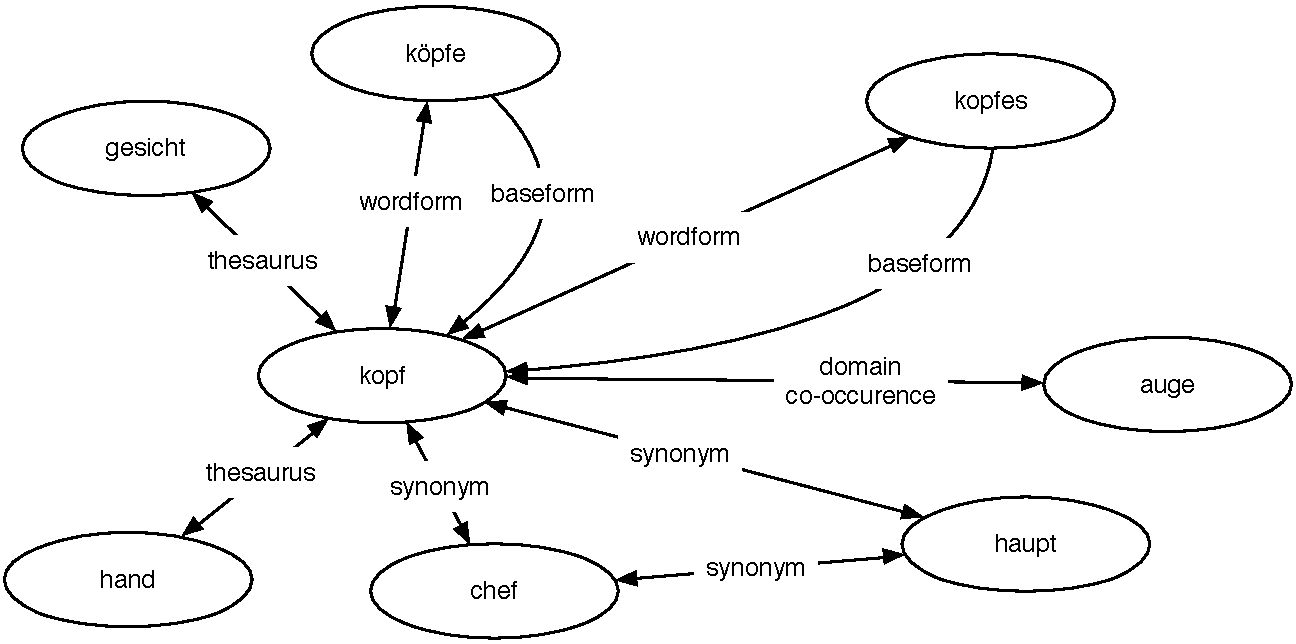
\includegraphics[width=0.8\textwidth]{wortschatz_transformation}
\caption{Beispiel--Graphausschnitt der transformierten Wortschatz--Daten}
\label{fig:wortschatz_transformation}
\end{figure}

Einen Sonderfall stellen die Kategorien der Wörter dar. Diese können in der vorliegenden Form nicht direkt zur Link Discovery genutzt werden. Daher werden diese Daten mittels der Ermittlung von Kookkurrenzen umgeformt. Dabei ist die Kookkurrenz zweier Begriffe durch die gemeinsame Einordnung in Kategorien definiert. Somit werden bei der Transformation mittels Kookkurrenzberechnung Kanten mit den Kookkurrenzmaßen aus \cref{measures} und dem Kantentyp \emph{Kategorie--Kookkurrenz} erzeugt.

Zusammenfassend werden bei der Transformation demnach Kanten mit den Typen \emph{Synonym}, \emph{Thesaurus}, \emph{Wortform}, \emph{Grundform} und \emph{Kategorie--Kookkurrenz} erzeugt. In \cref{fig:wortschatz_transformation} wird beispielhaft ein Ausschnitt des resultierenden Graphen gezeigt. Dabei fällt auf, dass mit Ausnahme der Grundform--Kanten jede Kante in beide Richtungen existiert. Dies ist der Art der Beziehungen geschuldet, da diese in beide Richtungen gültig sind.

\subsection{Integration}

Zur Integration wird der im Transformationsschritt erzeugte Graph mit dem vorhandenen Graphen vereinigt. Diese Vereinigung wird analog zur Integration der Daten des Clicktracking--Systems in \cref{click_integration} durchgeführt. 

\subsection{Ergebnisse}

Insgesamt wurden dadurch \num{145023} neue Knoten und \num{50227965} neue Kanten erzeugt.  Dabei entfallen \num{48399466} Kanten auf Kookkurrenz von Kategorien, \num{550270} Kanten auf Wortformen, \num{149381} Kanten auf Grundformen, \num{279118} Kanten auf Synonyme und \num{849730} Kanten auf Thesaurus--Beziehungen.

In \cref{fig:hist_only_wortschatz} ist die Verteilung durch die Integration des Wortschatzes erzeugten Kanten also Histogramm mit exponentiell wachsenden Klassen abgebildet. \cref{tab:only_wortschatz} zeigt statistische Kennzahlen dieser Verteilung.

\begin{figure}[h]
\centering
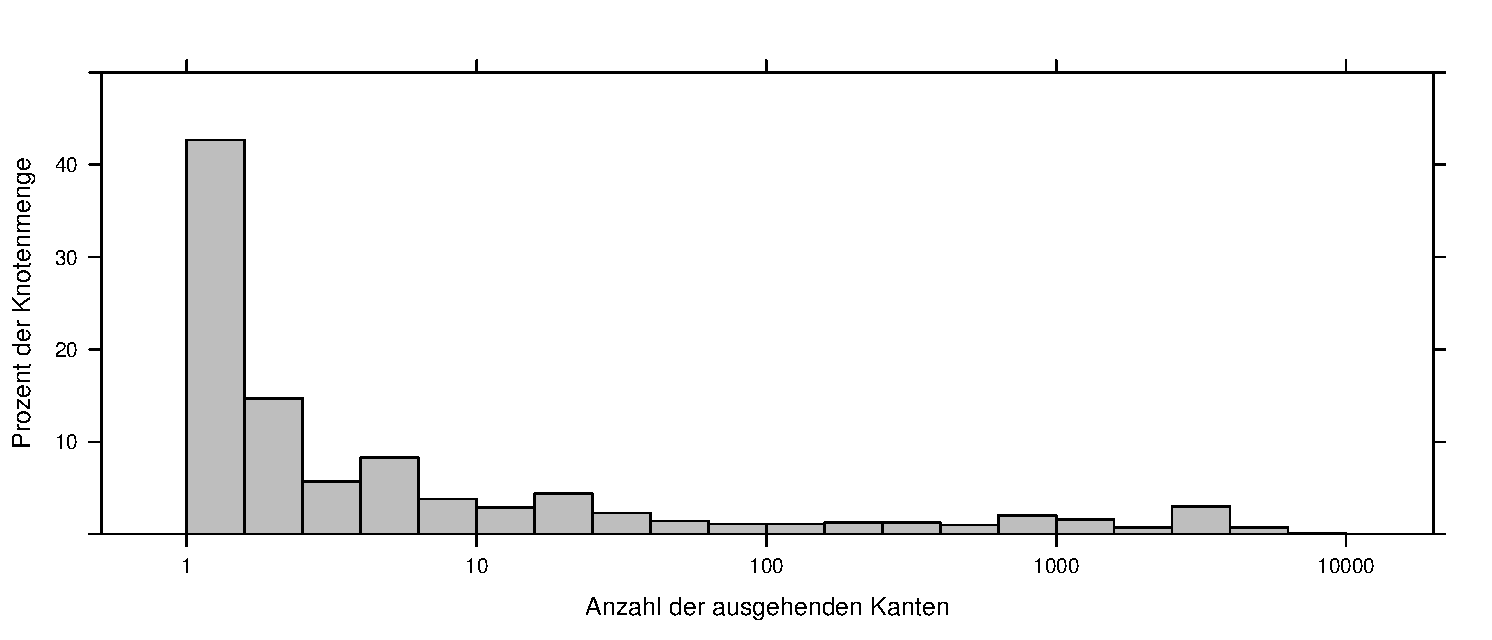
\includegraphics[width=\textwidth]{hist_only_wortschatz}
\caption{Histogramm der Verteilung der Wortschatz--Kanten}
\label{fig:hist_only_wortschatz}
\end{figure}

\begin{table}[h]
\centering
\begin{tabular}{lr}
    \toprule
    Kennzahl & Wert \\
    \midrule
    \(min\) & \num{1} \\
    \(Q_{0.25}\) & \num{1} \\
    \(Q_{0.5}\) & \num{2} \\
    \(Q_{0.75}\) & \num{10} \\
    \(max\) &  \num{11020} \\
    \(avg\) &  \num{203,8} \\
    \bottomrule
\end{tabular}
\caption{Statistische Kennzahlen für die Verteilung der Wortschatz--Kanten}
\label{tab:only_wortschatz}
\end{table}

Bei Inspektion der Daten fällt auf, dass der Großteil der betroffenen Knoten nur eine Wortschatz--Kante besitzt. Jedoch deutet der Hohe Durchschnitt, verbunden mit dem \(Q_{0.75}=10\) darauf hin, dass im Gegensatz zu den anderen Integrationsschritten deutlich mehr Knoten existieren, die viele Kanten besitzen.

Nachdem alle Anreicherungsschritte durchgeführt und beschrieben wurde, beschäftigt sich der nächste Abschnitt mit den zusammengefassten Ergebnissen der Integrations-- und Anreicherungsschritte.

\section{Ergebnisse der Integrations-- und Anreicherungsschritte}
\label{lda_results}

In den bisherigen Auswertungen der Integrations-- und Anreicherungsschritte wurden lediglich die Eigenschaften der vom jeweiligen Schritt betroffenen Begriffe analysiert. Dieser Abschnitt beschäftigt sich mit der Veränderung des durch den Graphen repräsentierten Weltausschnittes bei jedem durchgeführten Link--Discovery--Schritt.

\subsection{Anzahl der Knoten und Kanten}

\cref{tab:discovery_amounts} zeigt zusammengefasst die quantitative Veränderung des Graphen nach jedem durchgeführten Schritt. Dabei zeigt sich, dass die Integration der Daten des Wortschatzes mit Abstand die meisten neuen Kanten in den Graphen eingefügt hat. 

\begin{table}[h]
\centering
\begin{tabular}{lrcr}
    \toprule
    Schritt & Knoten & \phantom{abc} & Kanten \\
    \midrule
    Tags & \num{314351} && \num{21834868} \\
    Clicktracking & \num{78237} && \num{310860} \\
    Zerlegung & \num{38349} && \num{1238900} \\
    Wortschatz & \num{145023} && \num{50227965} \\
    \midrule
    Gesamt & \num{575960} && \num{73612593} \\
    \bottomrule
\end{tabular}
\caption{Entwicklung der Knoten-- und Kantenanzahl nach jedem Link--Discovery--Schritt}
\label{tab:discovery_amounts}
\end{table}

Bei der Verwendung der Clicktracking--Daten wurden im Verhältnis wenig neue Knoten und Kanten erzeugt. Dies ist im Wesentlichen auf den zum Zeitpunkt des Importes noch geringen Datenbestand zurückzuführen. Daher sollte dieser Schritt zukünftig wiederholt werden, da mit der längeren Laufzeit des Clicktracking--Systems auch ein größeres Potential für neue Verknüpfungen vorhanden ist.

\subsection{Kantenverteilung}

Neben der absoluten Anzahl der Knoten und Kanten sind bei einer Betrachtung der quantitativen Ergebnisse auch die Anzahl der Kanten, die von einem Knoten ausgehen, von Interesse. Diese Verteilung der Kanten je Knoten nach jedem Schritt ist in den \cref{fig:hist_after_tags,fig:hist_after_clicktracking,fig:hist_after_decomposition,fig:hist_after_wortschatz} als Histogramm dargestellt.

\begin{figure}[p]
\centering
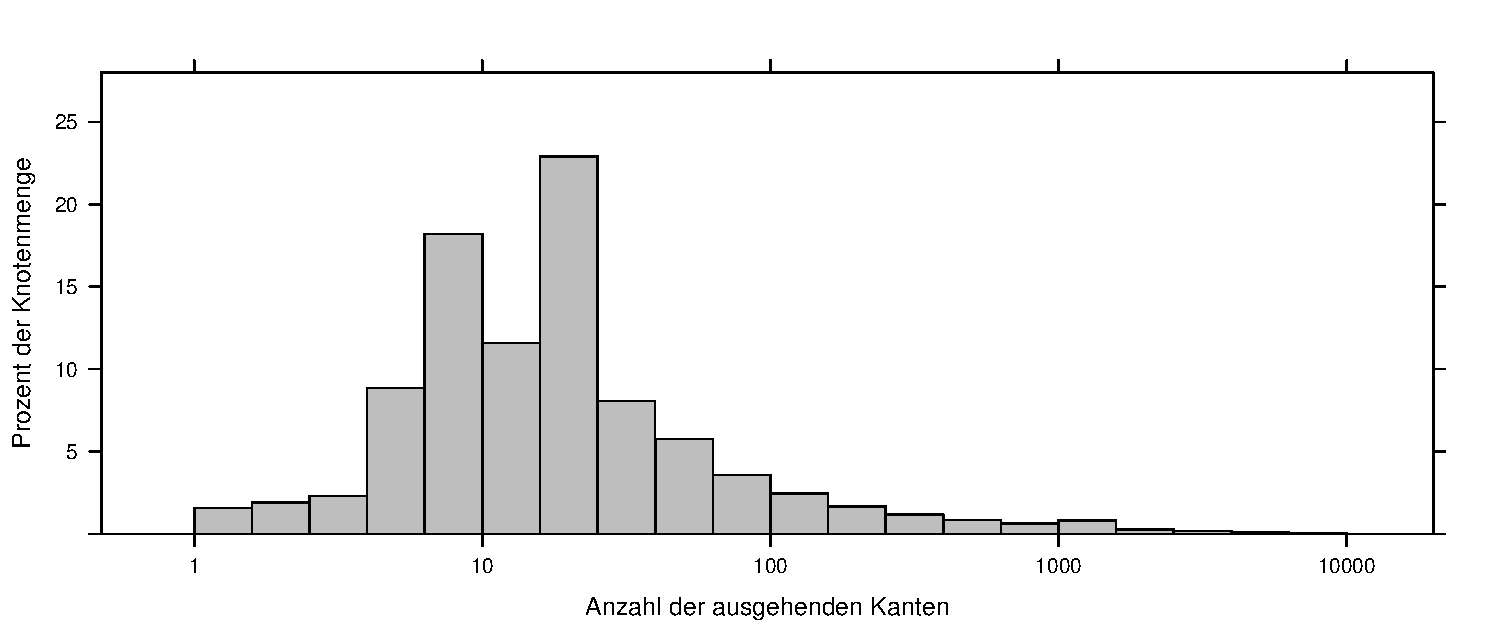
\includegraphics[width=0.65\textwidth]{hist_after_tags}
\caption{Histogramm der Kantenverteilung nach Integration der Tagging--Daten}
\label{fig:hist_after_tags}
\end{figure}

\begin{figure}[p]
\centering
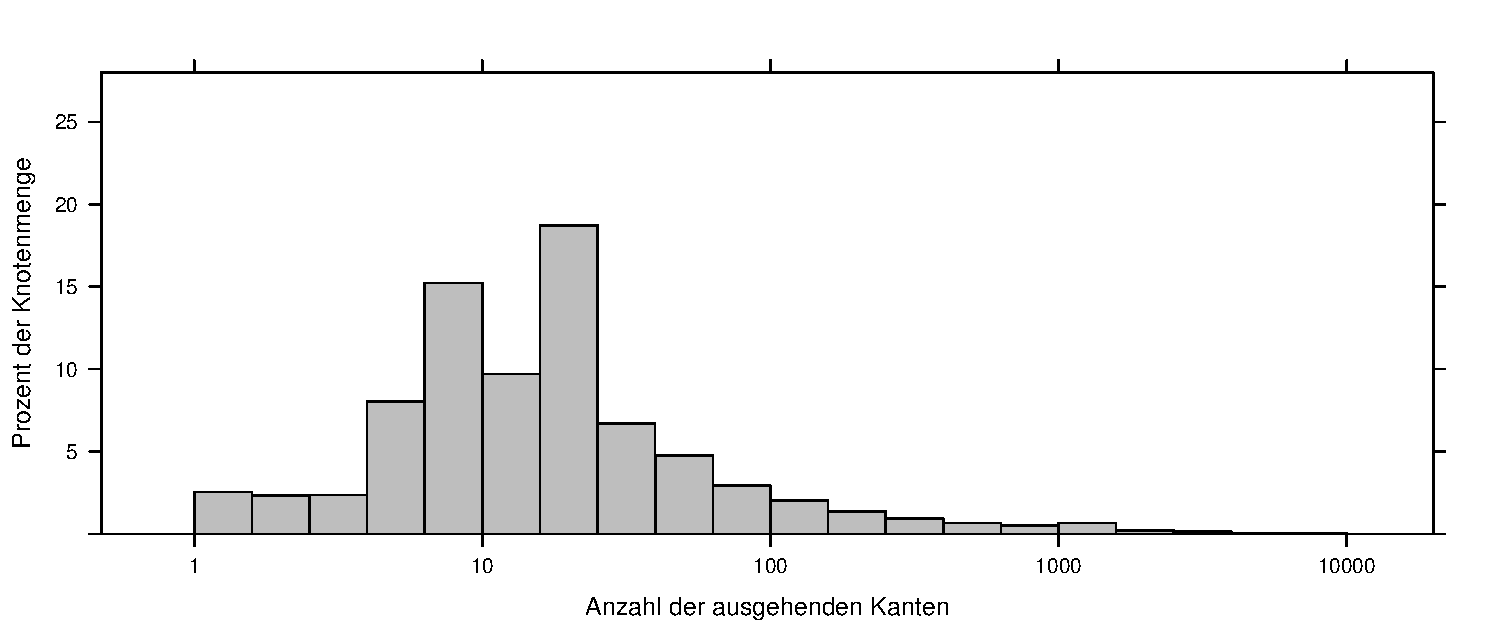
\includegraphics[width=0.65\textwidth]{hist_after_clicktracking}
\caption{Histogramm der Kantenverteilung nach Integration der Clicktracking--Daten}
\label{fig:hist_after_clicktracking}
\end{figure}

\begin{figure}[p]
\centering
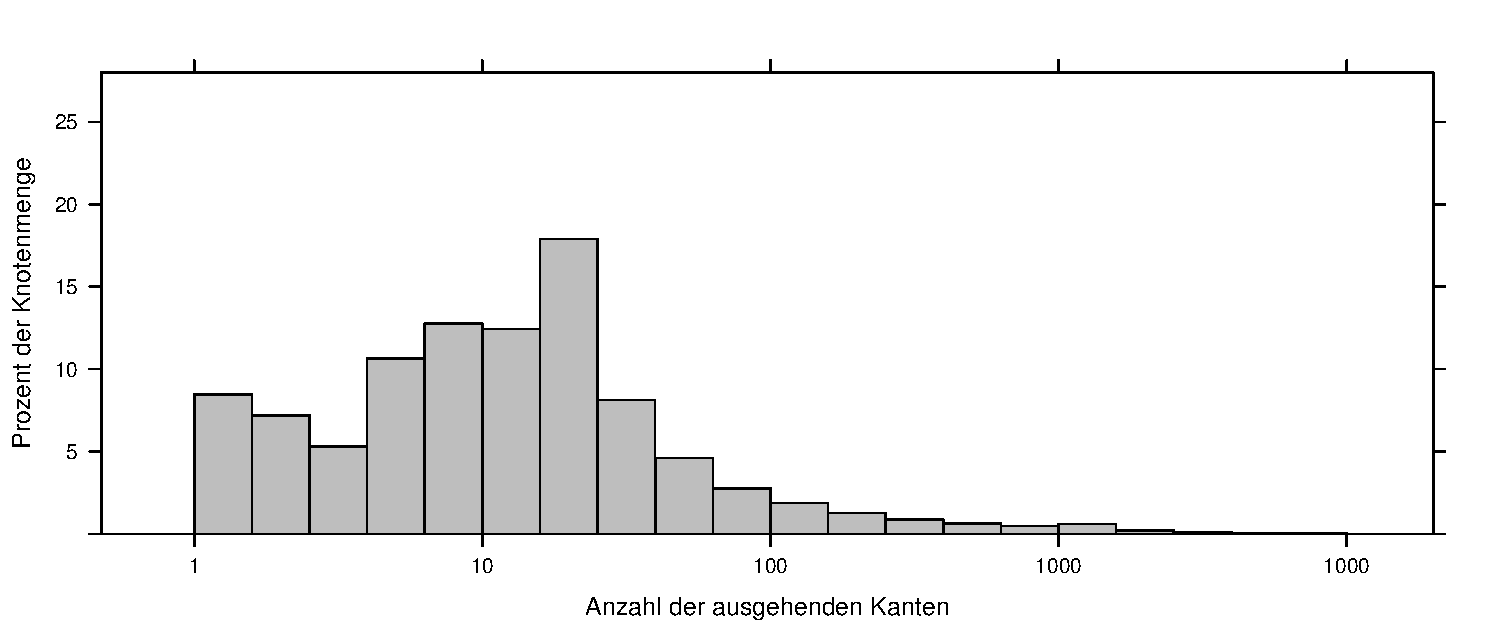
\includegraphics[width=0.65\textwidth]{hist_after_decomposition}
\caption{Histogramm der Kantenverteilung nach der Zerlegung von Wortgruppen}
\label{fig:hist_after_decomposition}
\end{figure}

\begin{figure}[p]
\centering
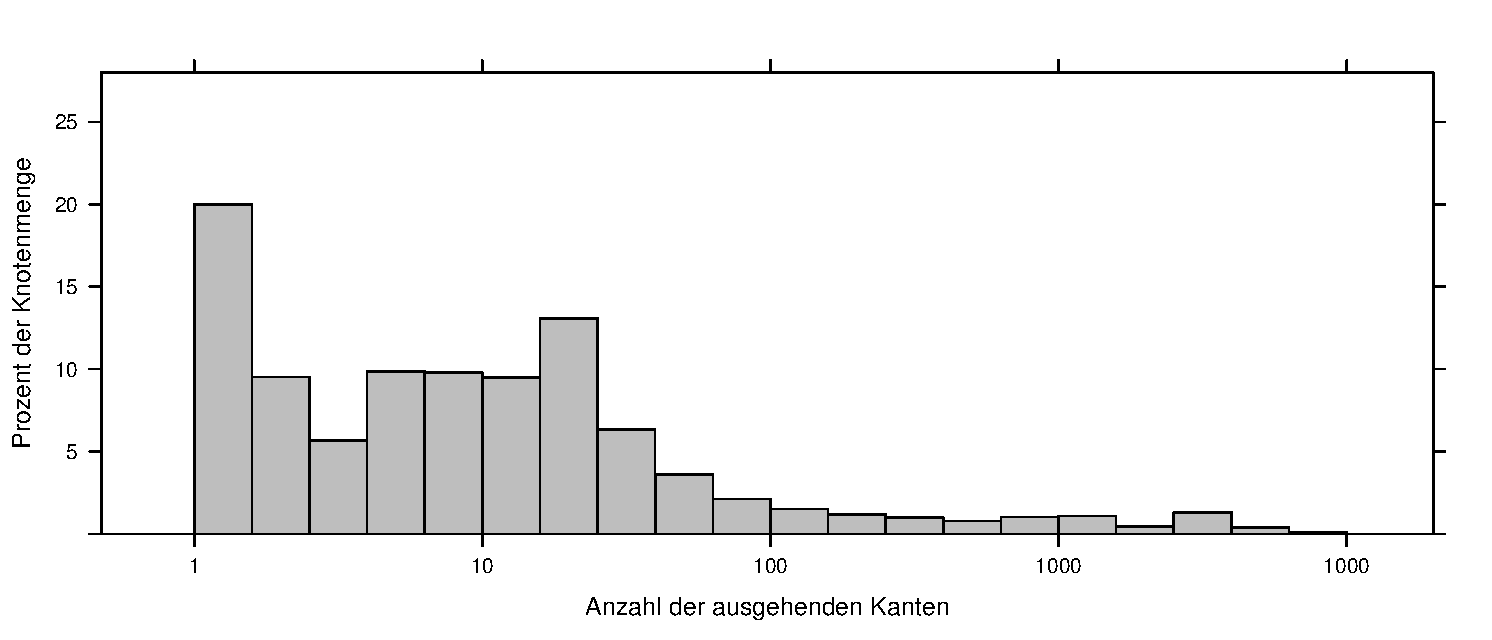
\includegraphics[width=0.65\textwidth]{hist_after_wortschatz}
\caption{Histogramm der Kantenverteilung nach Integration der Wortschatz--Daten}
\label{fig:hist_after_wortschatz}
\end{figure}

\begin{table}[h]
\centering
\begin{tabular}{lrrrrrr}
    \toprule
    Schritt & \(min\) & \(Q_{0.25}\) & \(Q_{0.5}\) & \(Q_{0.75}\) & \(max\) & \(avg\) \\
    \midrule
    Tags & \num{0} & \num{8} & \num{15} & \num{26} & \num{35170} & \num{69,64} \\
    Clicktracking & \num{0} & \num{3} & \num{10} & \num{23} & \num{35170} & \num{56,41} \\
    Zerlegung & \num{0} & \num{4} & \num{11} & \num{24} & \num{37940} & \num{54,26} \\
    Wortschatz & \num{0} & \num{2} & \num{8} & \num{23} & \num{38380} & \num{127,8} \\
    \bottomrule
\end{tabular}
\caption{Statistische Kennzahlen der Kantenverteilung nach jedem Link--Discovery--Schritt}
\label{tab:discovery_edges_per_node}
\end{table}

\cref{tab:discovery_edges_per_node} zeigt die einige statistische Kennzahlen der Kantenverteilung nach jedem Schritt. Dabei sind das Minimum, das untere, mittlere (Median) und obere Quartil, das Maximum und der Durchschnitt dargestellt.

Auffällig ist hierbei, dass die Integration von Clicktracking- und Wortschatz--Daten zu einer Herabsetzung des Medians führten. Dies bedeutet, dass nach Durchführung dieser Schritte verhältnismäßig weniger viel verbundene Knoten im Datenbestand existierten als davor. Jedoch deutet die Entwicklung des Durchschnittes nach der Integration der Wortschatz--Daten darauf hin, dass die Knotenanzahl viel verbundener Knoten nach diesem Schritt deutlich größer geworden ist.

Das Absinken des Durchschnittes nach Integration der Clicktracking--Daten kann in der geringen Menge der Daten begründet werden. Durch die geringe Anzahl von Kookkurrenzen konnten viel verbundene Knoten keinen relevanten Zugewinn an Verbindungen verzeichnen, während für wenig verbundene Knoten verhältnismäßig mehr neue Verbindungen hinzukamen.

Die Entwicklung der Verteilung zeigt, dass der Anteil wenig verbundener Knoten an der Knotenmenge ständig gewachsen ist. Daraus kann geschlussfolgert werden, mit jedem Schritt mehr Knoten existierten, die überhaupt Verbindungen besitzen. Speziell die Integration der Wortschatz--Daten hat gleichzeitig den Anteil der wenig verbundenen als auch der viel verbundenen Knoten erhöht.

Generell lässt sich festhalten, dass die Anzahl viel verbundener Knoten gemessen an der Gesamtanzahl relativ klein ist. Die Auswirkungen dessen hängen jedoch stark von der Anwendung der Daten ab und sind im Rahmen dieser Arbeit nicht beurteilbar.

Nach der quantitativen Auswertung der Link--Discovery--Schritte wird im nächsten Abschnitt die konkret durchgeführte Priorisierung der Beziehungen beschrieben.

\section{Priorisierung der Beziehungen}

Im Folgenden wird beschrieben, wie die in den Abschnitten \labelcref{ld_tags,clicktracking,decomposition,wortschatz} durch Link Discovery erzeugten Beziehungen zwischen den Begriffen des Weltausschnittes prioirisiert wurden. Der Prozess der Prioisierung folgt dabei grundsätzlich dem in \cref{prio_evo} skizzierten Prozess unter Zuhilfenahme evolutionärer Algorithmen. Dazu wird die Vorgehensweise und die Implementierung der Komponenten des evolutionären Algorithmus erläutert und die Ergebnisse ausgewertet.

Zum Zeitpunkt der Priosierung befanden sich neun verschiedene Beziehungstypen im Weltausschnitt: \emph{Tag--Kookkurrenz}, \emph{Klick--Kookkurrenz}, \emph{Kategorie--Kookkurrenz}, \emph{Zusammensetzung}, \emph{Wortform}, \emph{Grundform}, \emph{Synonym}, \emph{Thesaurus--Beziehung} und \emph{Zerlegung}.

Der Prioisierungprozess versucht nun, diese Beziehungstypen gegeneinander zu gewichten, um für einen Anwendungsfall relevante Nachbarn eines Begriffes zu finden (siehe \cref{prioritization}). Dazu muss jedem Typ ein relatives Gewicht zu den anderen Typen zugeordnet werden. Beziehungen, die duch Kookkurrenz berechnet wurden, besitzen bereits aufgrund der angegebenen Kookkurrenzmaße ein Kantengewicht. Jedoch muss hierbei festgelegt werden, welches Maß für das Kantengewicht herangezogen werden und in welchem Verhältnis zu den Gewichten anderer Kantentypen es stehen soll.

Somit wird zum Zwecke der Priorisierung eine Gewichtung von zwölf verschiedenen Parametern gesucht. Der nächste Abschnitt beschäftigt sich mit dem zur Priorisierung implementierten evolutionären Algorithmus.

\subsection{Vorgehensweise}
\label{evo_implementation}

Zur Erläuterung der Vorgehensweise wird zum einen die Stichprobenauswahl, zum anderen die Komponenten Genotyp, Initialisierung, Selektion und Reproduktion des evolutionären Algorithmus (siehe \cref{evo_for_prio}) beschrieben.

\subsubsection{Stichprobenauswahl}

Zunächst sollte die Methode zur Auswahl der Stichproben erläutert werden. Insgesamt wurden fünfzehn Knoten ausgewählt, deren Beziehungen optimiert werden sollen. Die Auswahl der Knoten richtete sich nach der Popularität von Suchbegriffen auf der Website von Spreadshirt. Dazu wurden alle Begriffe mit mehr als eintausend Suchen herangezogen und diese nach Häufigkeit der Suchen geordnet. Daraus wurden zufällig je fünf Begriffe bis zum unteren Quartil, fünf Begriffe zwischen unterem und oberen Quartil und fünf Begriffe über dem oberen Quartil ausgewählt. Die ausgewählten Begriffe, deren Kantengewichtungen lokal optimiert werden sollen, lauten: \emph{Kopfkissenbezug}, \emph{Student}, \emph{Volkswagen}, \emph{Marathon}, \emph{Wow}, \emph{Krankenschwester}, \emph{Mountainbike}, \emph{Hammer}, \emph{Polska}, \emph{Regenbogen}, \emph{Minecraft}, \emph{Kind}, \emph{Dubstep}, \emph{Leipzig} und \emph{Valentinstag}.

Ziel dieser Auswahl war, eine möglichst vielfältige Verteilung der einzelnen Kantentypen zu erreichen, aus welcher sich nach Durchführung der Piorisierung möglicherweise Erkenntnisse ableiten lassen, ob die Piorisierung nur lokal oder auch global durchgeführt werden kann.

Nach Auswahl der Stichproben muss der Genotyp der am evolutionären Algorithmus teilnehmenden Individuen spezifiziert werden. Daraufhin muss definiert werden, wie die Komponenten des Algorithmus zu implementieren sind.

\subsubsection{Genotyp}

Jeder Lösungskandidat wird durch die Werte der zwölf Parameter definiert, die die Gewichtung der Kantentypen untereinander beeinflussen. Daher wird jedes Individuum als Objekt repräsentiert, dass zwölf Attribute besitzt. Davon sind neun Attribute reellwertig und drei Attribute vom Aufzählungstyp \emph{Kookkurrenzmaß}.

\begin{figure}
\centering
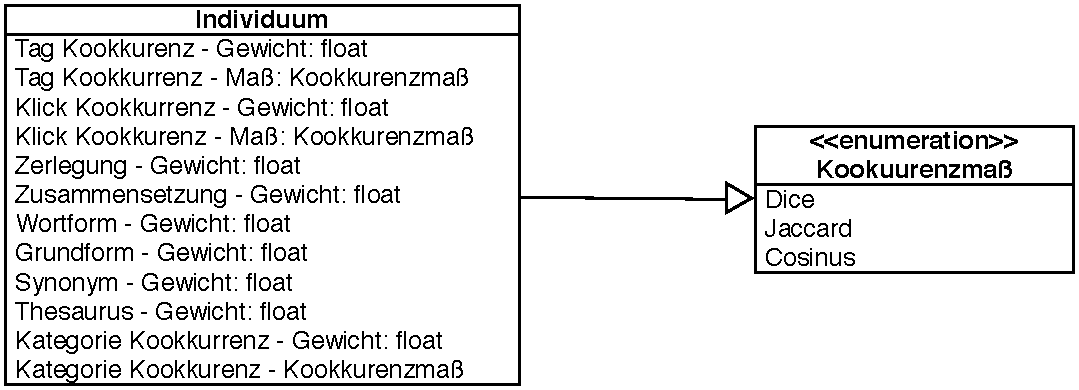
\includegraphics[width=0.9\textwidth]{genotype}
\caption{UML--Klassendiagramm des gewählten Genotyps}
\label{fig:genotype}
\end{figure}

Die reellwertigen Attribute stellen ein Gewicht des jeweiligen Kantentyps dar. Sie können nur relativ zu den anderen Kantengewichten betrachtet werden und somit nur im Rahmen der Optimierung von Interesse. Der Wertebereich dieser Attribute wird auf das Intervall \(W=[0,1] \in \mathbb{R}\) eingeschränkt. Die Kookkurrenzmaße entsprechen den in \cref{measures} genannten, also \emph{Dice}, \emph{Jaccard} und \emph{Kosinus}. Der Genotyp ist in \cref{fig:genotype} als UML--Klassendiagramm und in \cref{lst:genotyope} beispielhaft in JSON--Notation dargestellt.

\begin{lstlisting}[language=json, label={lst:genotyope}, caption={JSON--Beispiel für ein Individuum}, float=b]
{
    "tagCoOccMeasure" : 0,
    "tagCoOccWeight" : 0.6878115427680314,
    "clickCoOccMeasure" : 2,
    "clickCoOccWeight" : 0.1533144270069897,
    "synonymWeight" : 0.2355003503616899,
    "thesaurusWeight" : 0.9918724503368139,
    "baseformWeight" : 0.2843543488997966,
    "wordformWeight" : 0.93317318148911,
    "sharedDomainsMeasure" : 2,
    "sharedDomainsWeight" : 0.462230023695156,
    "compositionWeight" : 0.07963851140812039,
    "decompositionWeight" : 0.4740817183628678
}
\end{lstlisting}

\subsubsection{Initialisierung}

Im Initialisierungsschritt wird die anfängliche Population für jede der Stichproben gebildet. Dazu muss zuerst eine geeignet erscheinende Populationsgröße festgelegt werden.

In jeder Generation müssen im Selektionsschritt alle Individuen bewertet werden. Wie in \cref{prio_evo} bereits erläutert wurde, kann dies nur mit menschlicher Interaktion erfolgen. Somit sollte die Populationsgröße möglichst gering sein, um mit der gleichen Anzahl Bewertungen eine größere Anzahl von Generationen zu durchlaufen. Dies geschieht auf Kosten der Diversität in der Population. Jedoch wurde im Rahmen dieser Arbeit dieser Ansatz gewählt, um möglichst viele Möglichkeiten zu haben, die Parameter zu optimieren.

Es wurde eine Populationsgröße von zehn Individuen je Stichprobe gewählt. Somit müssen in jeder Generation einhundertfünfzig Individuen bewertet werden. Bei der Initialisierung wurden die Variablen jedes erzeugten Individuums zufällig gewählt.

\subsubsection{Selektion}

Die Bestimmung einer Fitnessfunktion für die Optimierung der Link Discovery gestaltet sich durch die Notwendigkeit menschlicher Beurteilung als schwierig. Eine solche Fitnessbestimmung müsste derart erfolgen, dass ein Benutzer jedem Individuum einen reellwertigen Fitnesswert zuweist. Dies gestaltet ist jedoch auf Grund der hohen Anzahl von Individuen nicht praktikabel.

Aus diesem Grund werden die Individuen, die in die nächste Generation übermommen werden, direkt durch den bewertenden Benutzer umgesetzt. Die umgesetzte Selektion erfolgt durch die Durchführung von Wettkämpfen. Hierzu werden in jeder Generation je fünf Paare von Individuen gebildet. Diese Paarungen stellen die Wettkämpfe dar, bei denen der Benutzer den Gewinner bestimmt. Alle Gewinner werden selektiert und im Reproduktionsschritt weiter verwendet.

Der Vorteil dieses Vorgehens ist, dass der Benutzer nur jeweils zwei Lösungskandidaten vergleichen muss, anstatt direkt fünf der zehn Individuen auszuwählen. Somit verringert sich der zu einem Zeitpunkt zu leistende kognitive Aufwand für die Selektion.

\begin{figure}
\centering
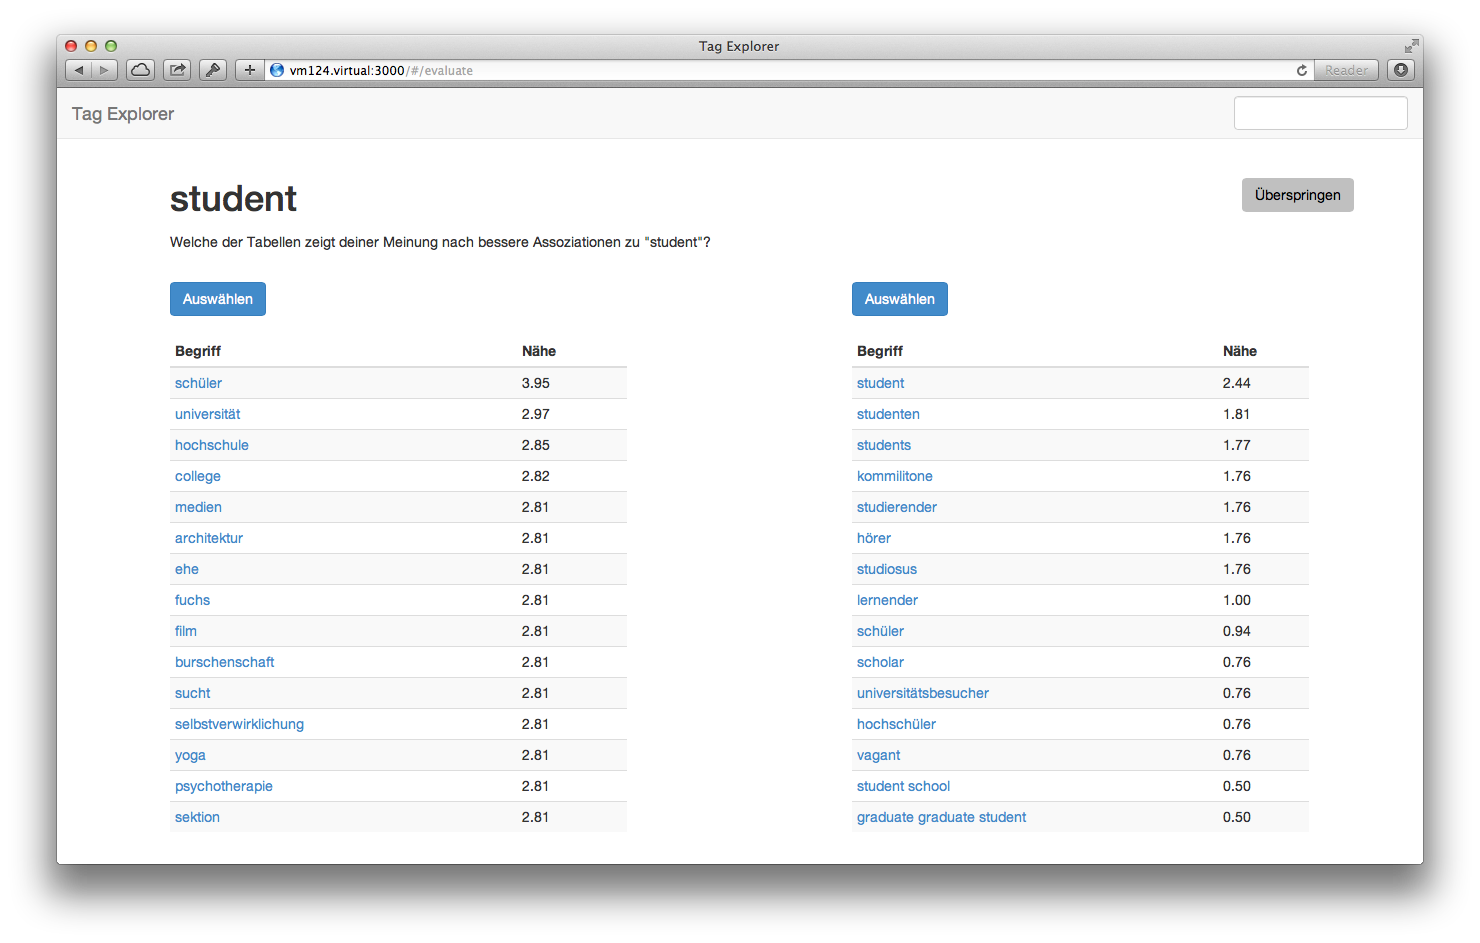
\includegraphics[scale=0.25]{eva_interface}
\caption{Screenshot der Oberfläche zur interaktiven Selektion}
\label{fig:eva_interface}
\end{figure}

Zur Selektion besucht der Benutzer eine Website, auf der ihm zwei Lösungskandidaten für eine Stichprobe präsentiert werden. Die Lösungskandidaten werden in Form von Listen von je fünfzehn Begriffen dargestellt, die die mit der jeweiligen Kantengewichtung erzeugten nächsten Nachbarn des Begriffes sind. Diese Oberfläche ist in \cref{fig:eva_interface} als Screenshot abgebildet. Nach Auswahl eines Gewinners wird dem Nutzer der nächste Wettkampf präsentiert.

Am Selektionsprozess kann sich jeder interessierte Benutzer beteiligen. Dieses Vorgehen wurde gewählt, um ein möglichst breites Spektrum an Meinungen bezüglich der Güte der Verbindungen zu erhalten.

Durch die direkte Auswahl beträgt die Reproduktionswahrscheinlichkeit für die ausgewählten Individuen eins und für die nicht ausgewählten Individuen Null \cite{sd2012}. Die gewählten Reproduktionsverfahren werden im nächsten Abschnitt beschrieben.

\subsubsection{Reproduktion}

Die fünf selektierten Individuen werden zur Reproduktion herangezogen, um fünf neue Individuen zu erzeugen, damit die Populationsgröße für die nächste Selektion wieder auf zehn Individuen steigt. Dazu werden die selektierten Individuen zuerst rekombiniert, um fünf Kindindividuen zu erzeugen, welche dann durch Mutation verändert werden.

\paragraph{Rekombination}

Als Verfahren zur Rekombination wurde der \emph{Ein--Punkt--Crossover} \cite{kw2007} gewählt. Dazu werden zufällig zwei Elternindividuen ausgewählt und ein zufälliger Crossover--Punkt berechnet. Werden die Genotypen der beiden Elternindividuen als Arrays dargestellt, werden bis zum Crossover--Punkt die Variablen des ersten Individuums, nach dem Crossover--Punkt die Variablen des zweiten Individuums übernommen. Der Crossover ist in \cref{fig:crossover} dargestellt.

\begin{figure}
\centering
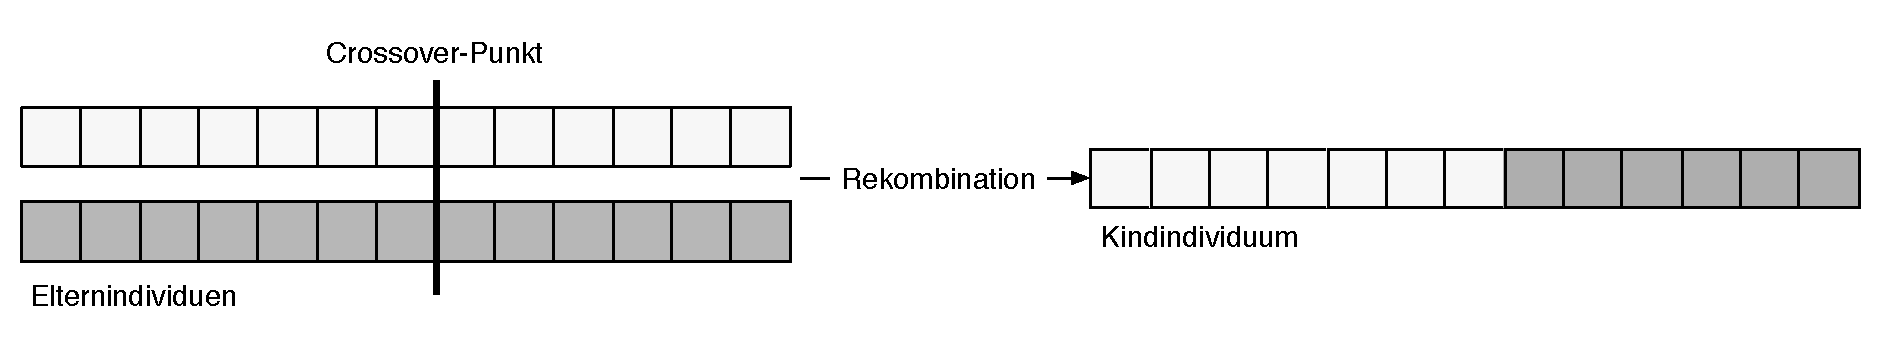
\includegraphics[width=\textwidth]{crossover}
\caption{Ein--Punkt--Crossover}
\label{fig:crossover}
\end{figure}

\paragraph{Mutation}

Zur Mutation der reellwertigen Kantengewichtungen wurde das Verfahren der \emph{Gauß-Mutation} \cite{kw2007} gewählt. Dabei wird zu jeder reellwertigen Variablen des Genotyps ein normalverteilter Zufallswert addiert. Verlässt der entstehende Wert das zulässige Intervall, so wird er auf die entsprechende Intervallschranke angepasst. Die Gauß-Mutation macht daher große Änderungen der Variable möglich, aber weniger Wahrscheinlich als kleine Änderungen. Sie eignet sich somit gut, um Diversität in der Population zu erzeugen. Konkret wurde in der Umsetzung der Prioisierung eine auf das Intervall \((0,1)\) angepasste Normalverteilung mit Erwartungswert \(\mu=0\) und Varianz \(\sigma=0.5\) gewählt. Die Variablen für die Kookkurrenzmaße werden nicht mutiert.

Nachdem in diesem Abschnitt die konkrete Umsetzung der Prioisierung mittels interaktiver evolutionärer Algorithmen beschrieben wurde, folgt im nächsten Abschnitt die Darstellung und Diskussion der Ergebnisse.

\subsection{Ergebnisse}

Die Optimierung wurde über insgesamt \num{13} Generationen durchgeführt. Somit wurden über alle Stichproben hinweg \num{975} Selektionen von Benutzern vorgenommen. Die Benutzer waren allesamt Mitarbeiter von Spreadshirt. Aufgrund der anonymen Teilnahme lässt sich nicht angeben, wie viele Einzelpersonen an der Optimierung teilgenommen haben.

\subsubsection{Kantengewichte}

Da nach jeder Selektion je Stichprobe fünf Individuen in der Population verbleiben, werden zunächst deren Kantengewichtungen untersucht. \cref{tab:winners_total} zeigt für jede Variable aus dem Genotyp den Median der in der dreizehnten Generation selektierten Individuen. Das Kantengewicht für den Typ \emph{Zerlegung} ist nicht in der Tabelle enthalten, da es sich bei den Stichproben nur um Einzelwörter handelt.

\begin{table}
\centering
\begin{tabular}{lcccccccc}
    \toprule
    Stichprobe & \(k_t\) & \(k_{kl}\) & \(s\) & \(t\) & \(g\) & \(w\) & \(k_{ka}\) & \(zu\) \\
    \midrule
    Dubstep & 0.85 & 0.60 & 0.53 & 0.77 & 1.00 & 1.00 & 1.00 & 0.48 \\
    Hammer & 0.81 & 0.56 & 0.88 & 0.45 & 1.00 & 0.89 & 0.00 & 0.59 \\
    Kind & 0.58 & 0.22 & 0.84 & 1.00 & 0.66 & 0.00 & 0.01 & 0.00 \\
    Kopfkissenbezug & 0.34 & 0.00 & 0.00 & 0.60 & 0.77 & 0.93 & 0.26 & 0.93 \\
    Krankenschwester & 1.00 & 0.20 & 0.28 & 0.60 & 0.70 & 0.88 & 0.59 & 0.33 \\
    Leipzig & 0.69 & 1.00 & 0.66 & 0.01 & 0.41 & 0.00 & 0.17 & 1.00 \\
    Marathon & 0.62 & 0.70 & 0.23 & 0.41 & 0.69 & 1.00 & 0.00 & 0.95 \\
    Minecraft & 0.71 & 0.34 & 0.31 & 0.38 & 0.74 & 1.00 & 0.00 & 1.00 \\
    Mountainbike & 0.34 & 0.48 & 0.00 & 0.00 & 1.00 & 1.00 & 0.85 & 0.00 \\
    Polska & 0.63 & 0.25 & 0.86 & 0.97 & 0.24 & 1.00 & 0.00 & 0.00 \\
    Regenbogen & 1.00 & 0.43 & 0.36 & 0.47 & 0.00 & 0.26 & 0.61 & 0.52 \\
    Student & 0.67 & 0.15 & 0.38 & 0.84 & 0.78 & 0.70 & 0.72 & 0.33 \\
    Valentinstag & 1.00 & 0.44 & 0.80 & 0.24 & 0.53 & 0.58 & 0.70 & 1.00 \\
    Volkswagen & 0.47 & 1.00 & 0.11 & 0.51 & 1.00 & 0.89 & 0.14 & 0.30 \\
    Wow & 0.08 & 1.00 & 0.93 & 0.21 & 1.00 & 0.54 & 0.53 & 0.68 \\
    \bottomrule
\end{tabular}
\caption{Mediane der Kantengewichte nach der finalen Selektion}
\caption*{
    \begin{tabular}{ll}
        \(k_t\) & Tag--Kookkurrenz\\
        \(k_{kl}\) & Klick--Kookkurrenz\\
        \(s\) & Synonyme \\
        \(t\) & Thesaurus \\
        \(g\) & Grundform \\
        \(w\) & Wortform \\
        \(k_{ka}\) & Kategorie--Kookkurrenz\\
        \(zu\) & Zusammensetzung\\
    \end{tabular}
}
\label{tab:winners_total}
\end{table}

Bei Betrachtung dieser Ergebnisse fällt auf, dass sich die Gewichtungen der Kanten von Stichprobe zu Stichprobe stark unterscheiden. Somit bestätigt sich die Vermutung, dass eine globale Optimierung der Kantengewichtungen keine sinnvollen Ergebnisse erzielt. Jedoch ergaben sich für die Typen \emph{Wortform} und \emph{Grundform} in allen Stichproben relativ hohe Gewichte.

\subsubsection{Kookkurrenzmaße}

In \cref{tab:measures_each} sind für alle Stichproben die nach der letzten Selektion jeweils am häufigsten in der Population auftretenden Kookkurrenzmaße aufgeführt.

\begin{table}
\centering
\begin{tabular}{llll}
    \toprule
    Stichprobe & Tags & Klicks & Kategorien \\
    \midrule
    Dubstep & Jaccard & Dice & Dice \\
    Hammer & Dice & Dice & Kosinus \\
    Kind & Kosinus & Dice & Kosinus \\
    Kopfkissenbezug & Dice & Dice & Kosinus \\
    Krankenschwester & Jaccard & Dice & Dice \\
    Leipzig & Jaccard & Jaccard & Kosinus \\
    Marathon & Dice & Dice & Jaccard \\
    Minecraft & Dice & Dice & Kosinus \\
    Mountainbike & Kosinus & Jaccard & Jaccard \\
    Polska & Jaccard & Dice & Kosinus \\
    Regenbogen & Dice & Dice & Jaccard \\
    Student & Dice & Dice & Dice \\
    Valentinstag & Dice & Jaccard & Kosinus \\
    Volkswagen & Kosinus & Dice & Dice \\
    Wow & Jaccard & Dice & Dice \\
    \bottomrule
\end{tabular}
\caption{Häufigste Kookkurrenzmaße nach der finalen Selektion}
\label{tab:measures_each}
\end{table}

\section{Zusammenfassung}
\chapter{Erstellung von Kookkurrenzgraphen}

\section{MapReduce}


\section{Anwendung von MapReduce zur Kookkurrenzberechnung}


Nachdem in diesem Kapitel die theoretischen Grundlagen für die Link Discovery mittels Kookkurrenz beschrieben wurden, beschäftigt sich das folgende Kapitel mit dem technischen System zur Umsetzung des Lösungsansatzes.
\chapter{Systembeschreibung}
\label{system}

Das nachfolgende Kapitel befasst sich mit der Beschreibung der Technologien und Vorgehensweisen, die zur Link Discovery im Rahmen dieser Arbeit angewendet wurden. Dazu zählen im Einzelnen die gewählte Datenbank MongoDB, das Datenmodell des Zielgraphen und das daraus resultierende Vorgehen und die Architektur des Systems zur Link Discovery.

\section{MongoDB}
\label{mongo}

Zur Umsetzung der Link Discovery wurde das Datenbankmanagementsystem MongoDB \cite{mo2013} gewählt. Bei MongoDB handelt es sich um eine quelloffene dokumentenorientierte Datenbank.

Im Gegensatz zu traditionellen relationalen Datenbanksystemen verzichtet MongoDB dabei auf eine tabellenförmige Struktur der Daten und speichert Datensätze in Form von so genannten \emph{Dokumenten}. Dabei handelt es sich um hierarchische Schlüssel-/Wertpaare, die schemalos in so genannten \emph{Collections} gespeichert werden. Schemalos bedeutet dabei, dass die Dokumente innerhalb einer Collection nicht alle dieselbe Struktur besitzen müssen.

Zur Repräsentation der Dokumente verwendet MongoDB ein Format, dass sich sehr an JSON \cite{json2006} anlehnt. JSON ist ein menschenlesbares Datenaustauschformat, das aus der Objektnotation der Programmiersprache JavaScript abgeleitet wurde. Das Datenformat von MongoDB ist BSON \cite{bson2013}, eine binäre Repräsentation von JSON, die einige zusätzliche Datentypen unterstützt. 

Listing \ref{lst:json} zeigt ein Beispiel für ein Dokument in MongoDB. Das Feld \emph{\_id} ist hierbei ein  Bezeichner vom Typ \emph{ObjectID}. Dieser stellt einen global eindeutigen Bezeichner dar, der benutzt werden kann, um Dokumente zu referenzieren. Innerhalb einer Collection ist \emph{\_id} dabei grundsätzlich eindeutig. Das Feld \emph{address} zeigt, dass Dokumente weitere Dokumente enthalten können. Das Feld \emph{friends} zeigt, dass Werte für Schlüssel auch Arrays von Werten sein können. Diese sind dabei nicht auf primitive Typen wie Zeichenketten oder Zahlen beschränkt, sondern können auch weitere Dokumente sein.

\begin{lstlisting}[language=json, label={lst:json}, caption={Ein Beispiel für ein Dokument in MongoDB}]
{
    "_id" : ObjectId("51efc20147cae77dfc02e0ac"),
    "name" : "Bob",
    "age": 25,
    "address": {
        "city": "Leipzig",
        "street": "Karl-Liebknecht-Str. 132"
        "zip": "04277"
    },
    "friends" : [
        "alice",
        "fred",
        "jason"
    ]
}
\end{lstlisting}

MongoDB unterstützt Anfragen über ein Binärprotokoll, welches über so genannte \emph{Treiber} in vielen Programmiersprachen abstrahiert zur Verfügung steht. Dabei sind vielfältige Lese- und Schreiboperationen möglich, die komplexe Abfragen und Operationen auf den gespeicherten Daten zulassen. Außerdem bietet MongoDB eine Implementierung des MapReduce-Programmiermodells (siehe \ref{mapreduce}) sowie die Möglichkeit, Indizes auf allen Hierarchieebenen der Dokumente zu nutzen. Für interaktive Operationen steht die \emph{Mongo Shell} zur Verfügung, welche Abfragen mittels der Programmiersprache JavaScript erlaubt und somit einen Treiber für diese Sprache darstellt.

Aufgrund der genannten Eigenschaften stellt MongoDB einen exzellenten Ausgangspunkt für die Link Discovery im Rahmen dieser Arbeit dar. Durch die vorhandene Schemaflexibilität können die Daten in der gerade benötigten Form gespeichert und abgefragt werden. Durch die Unterstützung von MapReduce mit mehreren Rechnern lassen sich Berechnungen wie die der Kookkurrenz (siehe \ref{mapreduce_cooccurence}) parallelisieren und somit beschleunigen.

Aus diesen Gründen stellt MongoDB das zentrale technische Element für die Link Discovery im Rahmen dieser Arbeit dar. Sobald die Daten aus den externen und internen Quellen in MongoDB importiert wurden, können die folgenden Schritte direkt mit Datenbankabfragen realisiert werden.

\section{Datenmodell}

Nach der Auswahl eines geeigneten Datenbanksystems sollte das Datenmodell des Ergebnisses genauer spezifiziert werden. Ist dieses vor der Link Discovery klar, können die einzelnen benötigten Schritte zur Erreichung des Zieles einfacher definiert werden.

Generell handelt es sich bei dem gewünschten Ergebnis um einen gerichteten Multigraph. Dieser repräsentiert Objekte, oder auch \emph{Knoten}, zwischen denen paarweise Verbindungen, die \emph{Kanten} bestehen. Die Besonderheit eines Multigraphen ist dabei, dass zwischen zwei Knoten auch mehrere Kanten existieren dürfen \cite{rd2012}. Dies ist dem gewählten Lösungsansatz geschuldet, da zwischen Wörtern und Wortgruppen verschiedenartige Beziehungen existieren können.

Somit müssen für das Datenmodell die beiden Entitäten \emph{Knoten} und \emph{Kante} modelliert werden.
Das komplette Datenmodell des Graphen nach der Integration aller Datenquellen ist in Anhang \ref{complete_data_model} dargestellt.

\subsection{Knoten}

Die Knoten repräsentierendie Wörter und Wortgruppen zwischen denen durch Link Discovery Verbindungen hergestellt werden sollen. Sie enthalten als benötigte Attribute eine Zeichenkette und ein Attribut Sprache. Die Kombination dieser beiden Attribute ist innerhalb der Knotenmenge eindeutig. Außerdem erhält jeder Knoten zur einfacheren Referenzierung einen eindeutigen Bezeichner.

Neben diesen immer vorhandenen Attributen kann ein Knoten beliebig viele weitere Eigenschaften besitzen. Diese Eigenschaften dienen dazu, den Begriffen, die die Knoten existieren, für spätere Verwendungen zusätzlichen Kontext zu geben. Im Wesentlichen definieren sich diese zusätzlichen Eigenschaften aus den Datenquellen, die zum Zweck der Link Discovery in den Graph integriert werden.

Zur besseren Kapselung und Übersicht sollten die zusätzlichen Eigenschaften in weitere Entitäten gekapselt werden. Die Struktur dieser zusätzlichen Typen kann dann zum Zeitpunkt der Integration der jeweiligen Datenquelle definiert werden.

Das resultierende Knotenmodell ist in Abbildung \ref{fig:node_erd} dargestellt.

\begin{figure}
\centering
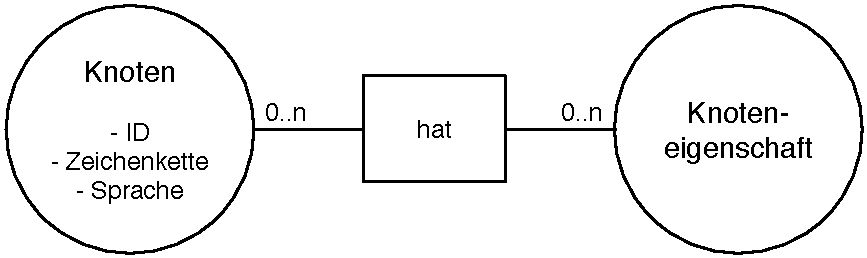
\includegraphics[width=0.6\textwidth]{node_erd}
\caption{Knotenmodell als Entity-Relationship-Diagramm}
\label{fig:node_erd}
\end{figure}

\subsection{Kanten}

Eine Kante ist im Wesentlichen durch die Knoten, die sie verbindet, beschrieben. Sie stellt einen irgendwie gearteten Zusammenhang zwischen zwei Knoten dar. Sie ist dabei gerichtet, um auch assymetrische Zusammenhänge zwischen Knoten abbilden zu können.

Somit sind die einzig immer benötigten Attribute der Quell- und Zielknoten und der Typ der Kante. Zusätzlich erhält jede Kante einen eindeutigen Bezeichner.

Alle weiteren Eigenschaften der Kante hängen vom Typ ab. Dies können beispielsweise Maße sein, die ein Kantengewicht darstellen. Da eine Kante nur genau einen Typ haben kann, werden die zusätzlichen Kanteneigenschaften einfach als Attribute an der Kante annotiert.

Das beschriebene Kantenmodell ist in Abbildung \ref{fig:edge_erd} dargestellt.

\begin{figure}
\centering
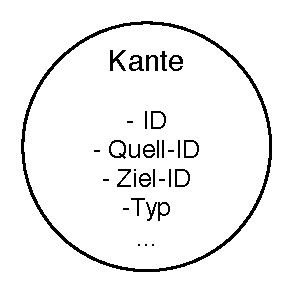
\includegraphics[width=0.2\textwidth]{edge_erd}
\caption{Kantenmodell als Entity-Relationship-Diagramm}
\label{fig:edge_erd}
\end{figure}

\subsection{Technische Umsetzung}

Um das beschriebene Datenmodell in MongoDB umzusetzen, muss es in eine Dokumentenform überführt werden. Dazu bietet sich an, Knoten in Kanten in unterschiedlichen Collections zu speichern, um sie voneinander zu trennen.

Somit stellt sich anschließend die Frage, wie die Knoten und Kanten als Dokumente repräsentiert werden. Durch die durch MongoDB gegebene Schemaflexibilität lassen sich die optionalen Eigenschaften von Knoten und Kanten direkt in den Dokumenten speichern.

Im Fall der Knoten bietet sich daher an, die zusätzlichen Eigenschaften als Unterdokumente des Knotens zu behandeln. Der Schlüssel für diese Unterdokumente ist dabei der Name der zusätzlichen Eigenschaft. Dadurch lassen sich die Knoten gut filtern, da die Abfrage auf das Vorhandensein des jeweiligen Schlüssels angepasst sein kann. Listing \ref{lst:node_json} zeigt ein Beispiel für einen Knoten in JSON-Notation. Arrays mit vielen Elementen sind dabei verkürzt dargestellt.

Die Kanten können direkt als Dokumente abgebildet werden. Über den Typ ergeben sich zusätzliche Eigenschaften. Listing \ref{lst:edge_json} zeigt beispielhaft ein Kantendokument für eine Tag-Kookkurrenz in JSON-Notation.

\begin{lstlisting}[language=json, label={lst:node_json}, caption={Knotendokument in JSON}]
{
    "_id" : ObjectId("51efc22447cae77dfc03e16b"),
    "language" : "de",
    "string" : "segeln",
    "languageDetection" : {
        "language" : "de",
        "confidence" : 1
    },
    "tagProperties" : {
        "occurenceCount" : 4678,
        "articleCount" : 2347,
        "designCount" : 2331,
        "articleIDs" : [ 
            4961057, 
            4977725, 
            ...
        ],
        "designIDs" : [ 
            1645572, 
            2216059, 
            ...
        ]
    },
    "wortschatzProperties" : {
        "synonyms" : [ 
            "flattern", 
            "fliegen", 
            "gaukeln", 
            ...
        ]
    }
}
\end{lstlisting}

\begin{lstlisting}[language=json, label={lst:edge_json}, caption={Kantendokument in JSON}]
{
        "_id" : ObjectId("51efd6f61177ff360605bd99"),
        "source" : ObjectId("51efc1af47cae77dfc00c3f8"),
        "target" : ObjectId("51efc1e047cae77dfc02087c"),
        "type" : "tag-co-occurence",
        "occurences" : 1,
        "dice" : 0.0001317089232795522,
        "jaccard" : 0.00006585879873551106,
        "cosine" : 0.008115343414514944
}
\end{lstlisting}

Nachdem die Datenformate definiert sind, beschäftigt sich das folgende Kapitel mit der Architektur des implementierten Link Discovery-Systems.

\section{Systemarchitektur}

Nach erfolgter Technologieauswahl und Modellierung der Daten soll im nächsten Abschnitt die Umsetzung der Link Discovery beschrieben werden.

Da die Mongo Shell eine vollwertige JavaScript-Laufzeitumgebung enthält und skriptbar ist, wurden die meisten Operationen im Rahmen dieser Arbeit als Skripte für diese Shell implementiert. Einzig der Import der Tag- und Clicktrackingdaten wurde mit Ruby-Skripten realisiert.

Die Schritte zur Link Discovery sind im Wesentlichen für jede zu integrierende Datenquelle gleich. Sie umfassen den Import, die Bereinigung, die Reduktion, die Transformation und die Integration der Daten \cite{hkp2012}.

\begin{figure}
\centering
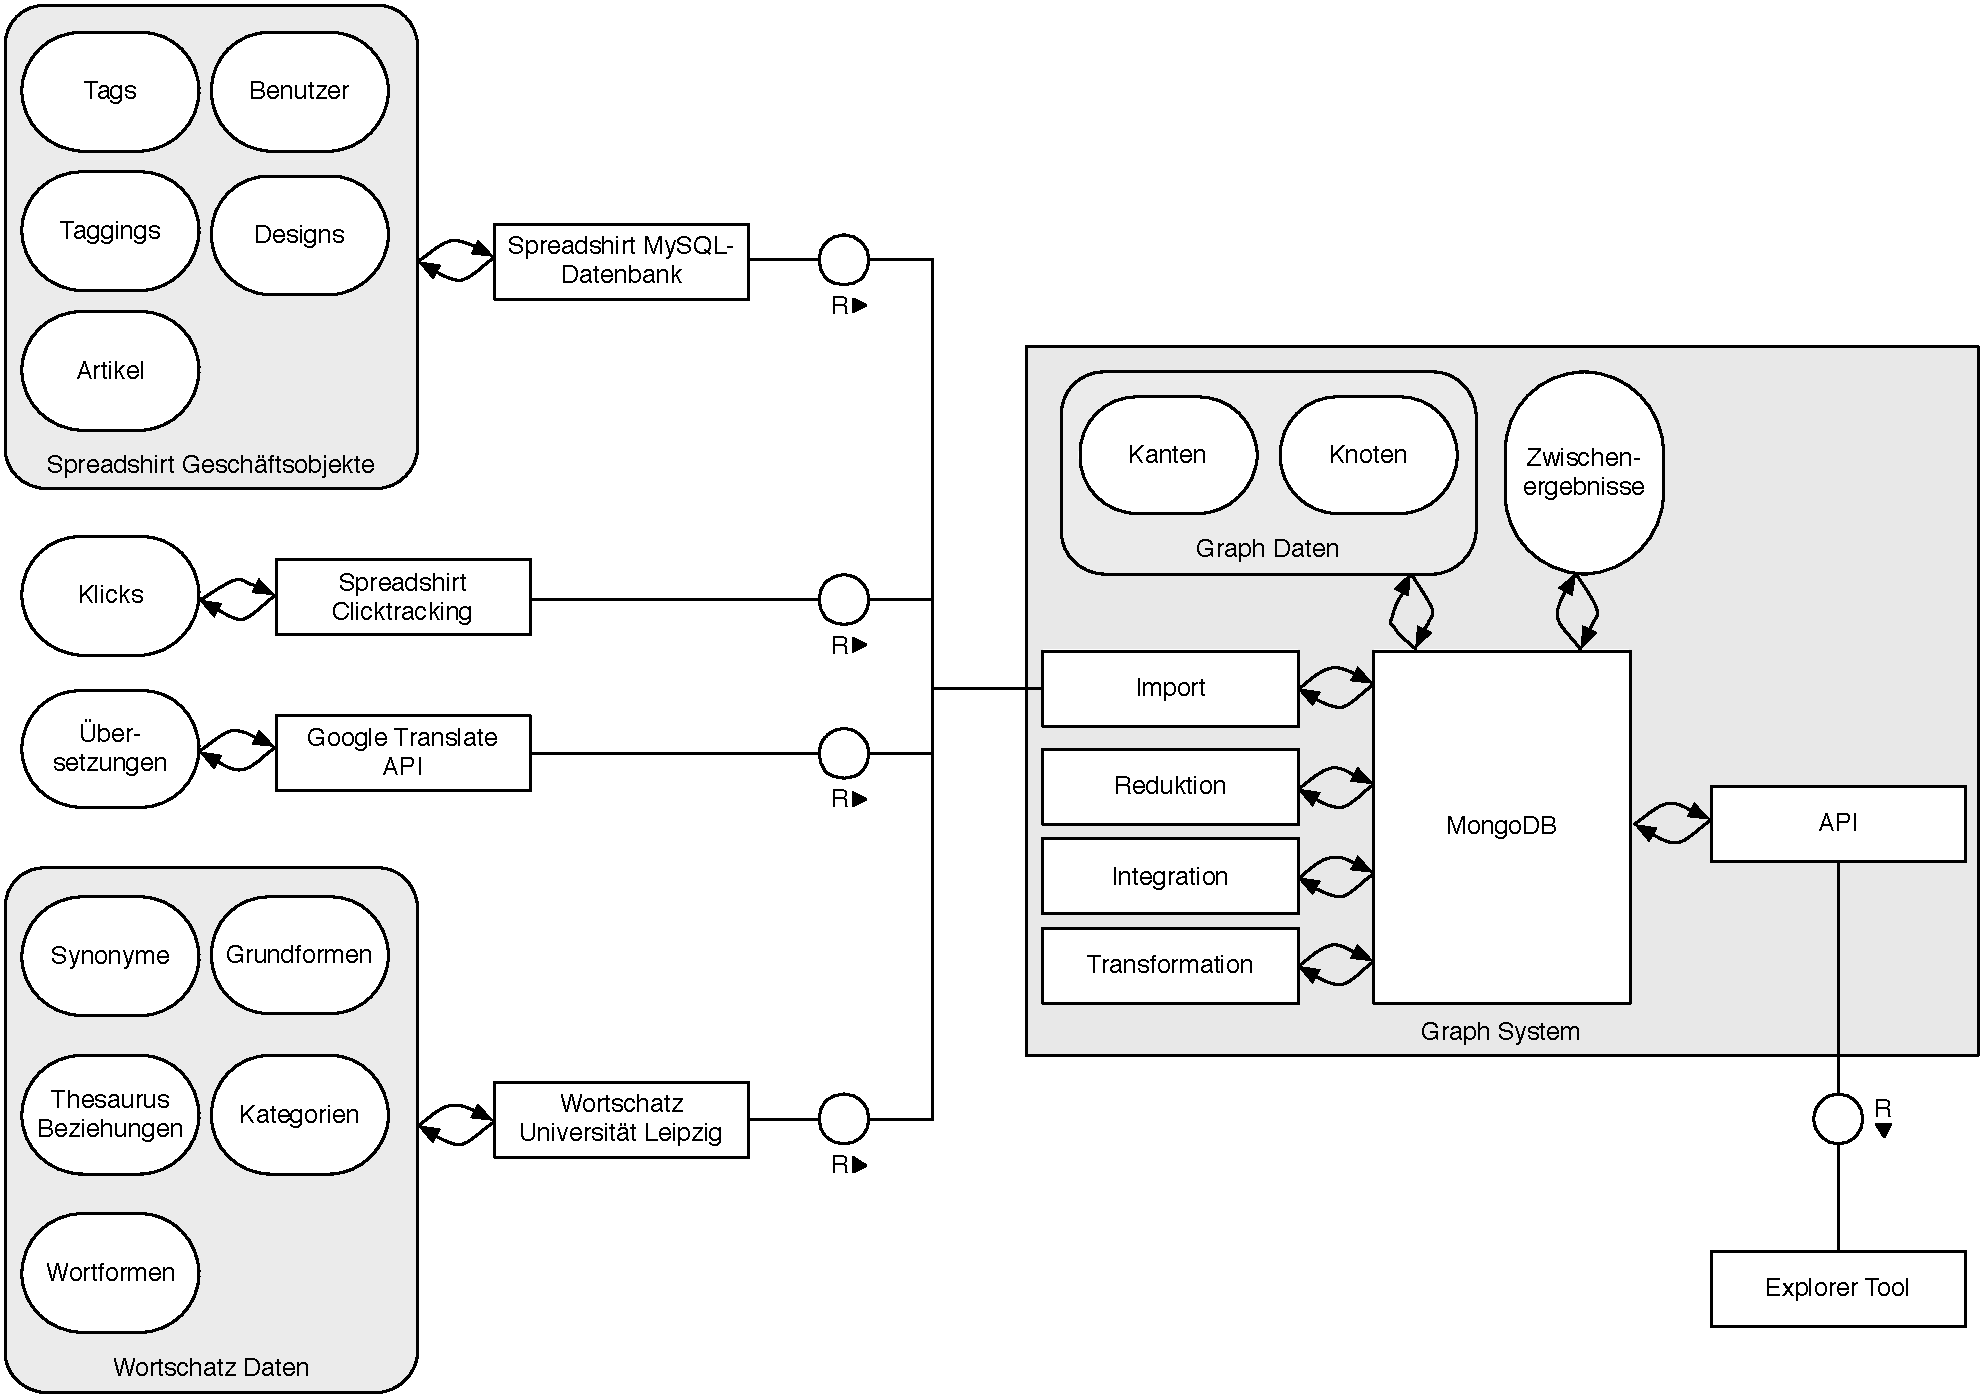
\includegraphics[width=1\textwidth]{architecture}
\caption{Systemarchitektur}
\label{fig:architecture}
\end{figure}

Abbildung \ref{fig:architecture} zeigt die komplette Architektur des implementierten Link Discovery Systems. Darin sind alle genutzten Datenquellen und die Daten, die sie bereit stellen, aufgeführt.

Für jede Datenquelle exisitiert ein Importskript, welches die Rohdaten importiert und in MongoDB speichert. Bei relationalen Datenquellen wie der Spreadshirt MySQL-Datenbank für die Tag-Daten wird pro Tabelle eine Collection und pro Zeile ein Dokument angelegt. Können nicht alle Daten importiert werden, wie beispielsweise bei der Wortschatz-API, kann das Importskript auch aufgrund der bisher im Graph vorhandenen Daten eine Auswahl an Anfragen an die externe Datenquelle erzeugen.

Im nachfolgenden Bereinigungsschritt werden die Daten so gut wie möglich von den in Abschnitt \ref{quality} beschriebenen Defekten befreit. Dazu zählen beispielsweise das Entfernen nicht nutzbarer Zeichen oder unvollständigen Datensätzen.

Der Reduktionsschritt dient zur Verkleinerung der Datenmenge. Dazu gehören beispielsweise Schritte zur Duplikatentfernung oder zur Auswahl relevanter Datensätze. In dieser Arbeit bestand die Haupteinschränkung der Datenmenge darin, nach Möglichkeit nur deutschsprachige Datensätze auszuwählen.

Der Schritt der Transformation überführt die Daten schließlich in eine Graphenform. Dies kann entweder über Kookkurrenz oder über eine andere, für die Art der importierten Daten geeignete, Methode erfolgen.

Das Integrationsskript für jede Datenquelle ist letztendlich für die Integration der Daten in den Zielgraphen verantwortlich. Dabei werden neue Informationen an die Knoten angefügt oder neue Kanten in den Graph integriert. In diesem Schritt passiert die Auflösung von eventuell vorhandenen temporären Bezeichnern in die entsprechenden im Graph vorhandenen eindeutigen Bezeichner.

Für die Abfrage der im Graph gespeicherten Informationen existiert außerdem eine API, welche Informationen zu Knoten und deren Nachbarn per HTTP als JSON-Dokumente zur Verfügung stellt. Diese API kann für die Einbindung der erzeugten Informationen in andere Applikationen genutzt werden. Über Anfrageparameter kann dabei die Gewichtung der einzelnen Kantentypen beeinflusst werden.

Eine Beispielanwendung, die die API des Link Discovery-Systems nutzt, ist der \emph{Tag Explorer}. Dabei handelt es sich um eine Browseranwendung, die die im Graph gespeicherten Beziehungen visualisiert und interaktiv erforschbar macht. Der Benutzer dieser Anwendung kann mit selbst gewählten Gewichtungen der Kanten den Graph durchsuchen. Außerdem werden, wenn vorhanden, über eine Anbindung der Spreadshirt-API zu der Zeichenkette des ausgewählten Knotens gefundene Designs angezeigt. In Abbildung \ref{fig:tag_explorer} ist ein Screenshot dieses Werkzeuges zu sehen.

\begin{figure}
\centering
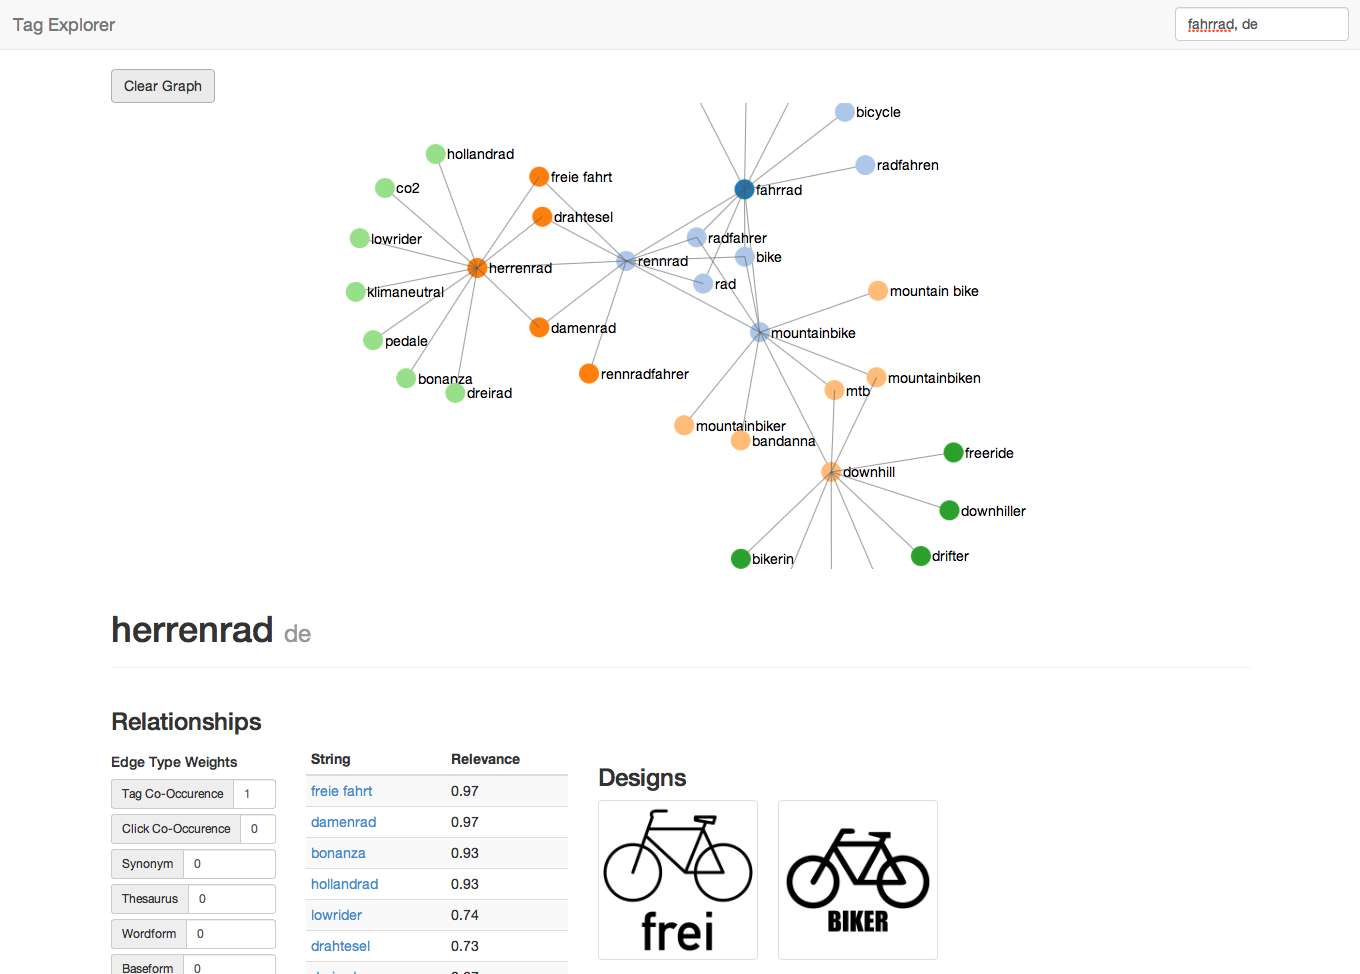
\includegraphics[width=0.9\textwidth]{tag_explorer}
\caption{Tag Explorer}
\label{fig:tag_explorer}
\end{figure}

Nachdem das System zur Link Discovery in diesem Kapitel beschrieben wurde, wird im nächsten Kapitel die praktische Durchführung und die Ergebnisse detailliert beschrieben.
\chapter{Schlussbetrachtung}
\label{summary}

In dieser Masterarbeit wurde ein Verfahren und dessen praktische Durchführung zum Finden von Zusammenhängen zwischen Begriffen, die \emph{Link Discovery}, beschrieben. Die Basis dafür stellten die Daten eines Tagging--Systems dar. Dazu wurden Tagging--Systeme grundlegend erläutert, deren Datenmodell definiert und die grundlegenden Unterschiede zwischen Folksonomies und geschlossenen Tagging--Systemen herausgearbeitet. Die Eigenschaften des im späteren Verlauf verwendeten Tagging--Systems von Spreadshirt wurden beschrieben und dessen Datenqualität in Hinblick auf Korrektheit, Vollständigkeit und Redundanzfreiheit diskutiert. Außerdem wurden die zu verarbeitenden Datenmengen definiert.

Für die Durchführung der Link Discovery wurde ein Framework definiert, welches die konzeptionelle Grundlage für die spätere Umsetzung darstellt. Dieses Framework modelliert den betrachteten Weltausschnitt, welcher Begriffe, den Kontext von Begriffen und deren Beziehungen untereinander enthält. Dieser Weltausschnitt wurde in eine Graphenrepräsentation überführt. Weiterhin wurde der Prozess der Link Discovery definiert und die einzelnen Schritte erläutert. Diese bestehen in der initialen Erstellung des Weltausschnittes, der Anreicherung durch Mining oder Integration weiterer Datenquellen und der Priorisierung der erzeugten Beziehungen. Die theoretischen Grundlagen von Kookkurrenz zur Beziehungserzeugung wurden definiert und die Berechnung veranschaulicht.

Weiterhin wurden mögliche Datenquellen diskutiert und die für die praktische Durchführung der Link Discovery in dieser Arbeit verwendeten Quellen ausgewählt. Diese bestehen aus dem Tagging-- und Clicktracking--System von Spreadshirt sowie dem Wortschatz der Universität Leipzig. Zur Priorisierung der erzeugten Beziehungen wurden evolutionäre Algorithmen erläutert und deren Einsatz im Rahmen der Priorisierung definiert.

Diese theoretischen Grundlagen wurden anschließend an konkreten Daten praktisch umgesetzt. Für jede integrierte Datenquelle wurden die Schritte Import, Bereinigung, Reduktion, Transformation in die Graphenrepräsentation und Integration in den Weltausschnitt ausführlich dargestellt und die quantitativen Ergebnisse präsentiert. Zur Anreicherung durch Mining wurde die Zerlegung von Wortgruppen in Einzelwörter erläutert. Im Anschluss wurden die quantitativen Veränderungen der Graphenrepräsentation nach jedem Link--Discovery--Schritt dargestellt und diskutiert. Nachdem alle Datenquellen integriert waren, wurde die praktische Umsetzung der Priorisierung der Beziehung mittels evolutionärer Algorithmen dargestellt und die Ergebnisse präsentiert.

Weiterhin wurden die Anforderungen an ein technisches System, welches die Link Discovery implementiert, formuliert und deren Umsetzung im Rahmen dieser Arbeit beschrieben. Dazu gehören die Wahl des Datenbanksystems MongoDB, die Implementierung der Komponenten in der Programmiersprache JavaScript und die Beschreibung von Kookkurrenzberechnung mittels des Programmiermodells MapReduce.

Die Ergebnisse dieser Arbeit stellen die Grundlage für weitere mögliche Arbeiten dar. Eine zukünftige Arbeit könnte sich mit der Auswertung der inhaltlichen Qualität der erzeugten Beziehungen beschäftigen. Dazu wird eine gründliche Analyse der integrierten Datenquellen und des Ergebnisses der Link Discovery mit Hilfe menschlicher Beurteilung benötigt.

Weiterhin sind Arbeiten denkbar, die die erzeugten Beziehungen für weitere Analyseverfahren nutzen. So könnten beispielsweise die Beziehungen zum Clustering der Begriffe zu Themen genutzt werden. Werden hierarchische Clusteringverfahren genutzt, können daraus Themenbäume und Topic Maps abgeleitet werden. Diese Themenbäume können sich durch ständige Durchführung der Link Discovery an aktuelle Trends in den Inhalten der betrachteten Website anpassen.

Der Link--Discovery--Prozess könnte durch einen interaktiven Trainingsschritt erweitert werden. In diesem Schritt wird die Beurteilung der Beziehungen durch Benutzer nicht nur zur Priorisierung, sondern zur direkten Veränderung des Weltausschnittes genutzt. Dabei werden Kanten eingefügt, die explizite statt nachträglich hergestellte Zusammenhänge beschreiben. Außerdem könnten durch manuellen Eingriff fehlerhafte Beziehungen gelöscht werden.

Insgesamt stellt das in dieser Arbeit beschriebene Framework eine gute Basis für Erweiterungen und neue Implementierungen dar. Das Verfahren ist flexibel und leistungsfähig genug, um auch auf anderen Datenbeständen gute Ergebnisse erzielen zu können. Durch Integration anderer Datenquellen und neuer Analyseverfahren kann die Qualität der gefundenen Zusammenhänge stetig verbessert werden. Die konkret erzeugten Daten bieten eine gute Grundlage für weitere Auswertungen und praktische Anwendungen.

\listoffigures
\listoftables
\lstlistoflistings

\sloppy
\printbibliography 

\end{document}